\documentclass[twoside]{book}

% Packages required by doxygen
\usepackage{fixltx2e}
\usepackage{calc}
\usepackage{doxygen}
\usepackage[export]{adjustbox} % also loads graphicx
\usepackage{graphicx}
\usepackage[utf8]{inputenc}
\usepackage{makeidx}
\usepackage{multicol}
\usepackage{multirow}
\PassOptionsToPackage{warn}{textcomp}
\usepackage{textcomp}
\usepackage[nointegrals]{wasysym}
\usepackage[table]{xcolor}

% NLS support packages
\usepackage[T2A]{fontenc}
\usepackage[russian]{babel}

% Font selection
\usepackage[T1]{fontenc}
\usepackage[scaled=.90]{helvet}
\usepackage{courier}
\usepackage{amssymb}
\usepackage{sectsty}
\renewcommand{\familydefault}{\sfdefault}
\allsectionsfont{%
  \fontseries{bc}\selectfont%
  \color{darkgray}%
}
\renewcommand{\DoxyLabelFont}{%
  \fontseries{bc}\selectfont%
  \color{darkgray}%
}
\newcommand{\+}{\discretionary{\mbox{\scriptsize$\hookleftarrow$}}{}{}}

% Page & text layout
\usepackage{geometry}
\geometry{%
  a4paper,%
  top=2.5cm,%
  bottom=2.5cm,%
  left=2.5cm,%
  right=2.5cm%
}
\tolerance=750
\hfuzz=15pt
\hbadness=750
\setlength{\emergencystretch}{15pt}
\setlength{\parindent}{0cm}
\setlength{\parskip}{3ex plus 2ex minus 2ex}
\makeatletter
\renewcommand{\paragraph}{%
  \@startsection{paragraph}{4}{0ex}{-1.0ex}{1.0ex}{%
    \normalfont\normalsize\bfseries\SS@parafont%
  }%
}
\renewcommand{\subparagraph}{%
  \@startsection{subparagraph}{5}{0ex}{-1.0ex}{1.0ex}{%
    \normalfont\normalsize\bfseries\SS@subparafont%
  }%
}
\makeatother

% Headers & footers
\usepackage{fancyhdr}
\pagestyle{fancyplain}
\fancyhead[LE]{\fancyplain{}{\bfseries\thepage}}
\fancyhead[CE]{\fancyplain{}{}}
\fancyhead[RE]{\fancyplain{}{\bfseries\leftmark}}
\fancyhead[LO]{\fancyplain{}{\bfseries\rightmark}}
\fancyhead[CO]{\fancyplain{}{}}
\fancyhead[RO]{\fancyplain{}{\bfseries\thepage}}
\fancyfoot[LE]{\fancyplain{}{}}
\fancyfoot[CE]{\fancyplain{}{}}
\fancyfoot[RE]{\fancyplain{}{\bfseries\scriptsize Создано системой Doxygen }}
\fancyfoot[LO]{\fancyplain{}{\bfseries\scriptsize Создано системой Doxygen }}
\fancyfoot[CO]{\fancyplain{}{}}
\fancyfoot[RO]{\fancyplain{}{}}
\renewcommand{\footrulewidth}{0.4pt}
\renewcommand{\chaptermark}[1]{%
  \markboth{#1}{}%
}
\renewcommand{\sectionmark}[1]{%
  \markright{\thesection\ #1}%
}

% Indices & bibliography
\usepackage{natbib}
\usepackage[titles]{tocloft}
\setcounter{tocdepth}{3}
\setcounter{secnumdepth}{5}
\makeindex

% Hyperlinks (required, but should be loaded last)
\usepackage{ifpdf}
\ifpdf
  \usepackage[pdftex,pagebackref=true]{hyperref}
\else
  \usepackage[ps2pdf,pagebackref=true]{hyperref}
\fi
\hypersetup{%
  colorlinks=true,%
  linkcolor=blue,%
  citecolor=blue,%
  unicode%
}

% Custom commands
\newcommand{\clearemptydoublepage}{%
  \newpage{\pagestyle{empty}\cleardoublepage}%
}

\usepackage{caption}
\captionsetup{labelsep=space,justification=centering,font={bf},singlelinecheck=off,skip=4pt,position=top}

%===== C O N T E N T S =====

\begin{document}

% Titlepage & ToC
\hypersetup{pageanchor=false,
             bookmarksnumbered=true,
             pdfencoding=unicode
            }
\pagenumbering{alph}
\begin{titlepage}
\vspace*{7cm}
\begin{center}%
{\Large Телецентр МИЭМ }\\
\vspace*{1cm}
{\large Создано системой Doxygen 1.8.13}\\
\end{center}
\end{titlepage}
\clearemptydoublepage
\pagenumbering{roman}
\tableofcontents
\clearemptydoublepage
\pagenumbering{arabic}
\hypersetup{pageanchor=true}

%--- Begin generated contents ---
\chapter{Алфавитный указатель групп}
\section{Группы}
Полный список групп.\begin{DoxyCompactList}
\item \contentsline{section}{Рекордер}{\pageref{group__recorder}}{}
\item \contentsline{section}{Сетка видеопотоков}{\pageref{group__grid}}{}
\item \contentsline{section}{Сетевой монитор}{\pageref{group__network__monitor}}{}
\end{DoxyCompactList}

\chapter{Алфавитный указатель пространств имен}
\section{Пространства имен}
Полный список пространств имен.\begin{DoxyCompactList}
\item\contentsline{section}{\hyperlink{namespacefrom-gsuite}{from-\/gsuite} }{\pageref{namespacefrom-gsuite}}{}
\item\contentsline{section}{\hyperlink{namespacegpio}{gpio} }{\pageref{namespacegpio}}{}
\item\contentsline{section}{\hyperlink{namespacenetwork__monitor}{network\+\_\+monitor} }{\pageref{namespacenetwork__monitor}}{}
\item\contentsline{section}{\hyperlink{namespacevideo-upload}{video-\/upload} }{\pageref{namespacevideo-upload}}{}
\end{DoxyCompactList}

\chapter{Иерархический список классов}
\section{Иерархия классов}
Иерархия классов.\begin{DoxyCompactList}
\item \contentsline{section}{Audio\+Source}{\pageref{struct_audio_source}}{}
\item \contentsline{section}{network\+\_\+monitor.\+Camera}{\pageref{classnetwork__monitor_1_1_camera}}{}
\item \contentsline{section}{Camera}{\pageref{struct_camera}}{}
\item \contentsline{section}{Config}{\pageref{class_config}}{}
\item \contentsline{section}{UI\+:\+:display\+\_\+player\+\_\+data}{\pageref{struct_u_i_1_1display__player__data}}{}
\item \contentsline{section}{UI\+:\+:gdrive\+\_\+status\+\_\+data}{\pageref{struct_u_i_1_1gdrive__status__data}}{}
\item \contentsline{section}{network\+\_\+monitor.\+Grapher}{\pageref{classnetwork__monitor_1_1_grapher}}{}
\item \contentsline{section}{Pad\+Data}{\pageref{struct_pad_data}}{}
\item \contentsline{section}{Player}{\pageref{class_player}}{}
\item Q\+Main\+Window\begin{DoxyCompactList}
\item \contentsline{section}{network\+\_\+monitor.\+U\+I\+Menu}{\pageref{classnetwork__monitor_1_1_u_i_menu}}{}
\end{DoxyCompactList}
\item Q\+Widget\begin{DoxyCompactList}
\item \contentsline{section}{network\+\_\+monitor.\+U\+I\+Graph}{\pageref{classnetwork__monitor_1_1_u_i_graph}}{}
\end{DoxyCompactList}
\item \contentsline{section}{Recorder}{\pageref{class_recorder}}{}
\item \contentsline{section}{Recording}{\pageref{class_recording}}{}
\item \contentsline{section}{Room}{\pageref{class_room}}{}
\item \contentsline{section}{UI\+:\+:switch\+\_\+state\+\_\+changed\+\_\+data}{\pageref{struct_u_i_1_1switch__state__changed__data}}{}
\item \contentsline{section}{UI}{\pageref{class_u_i}}{}
\item Q\+Runnable\begin{DoxyCompactList}
\item \contentsline{section}{network\+\_\+monitor.\+Pinger}{\pageref{classnetwork__monitor_1_1_pinger}}{}
\end{DoxyCompactList}
\end{DoxyCompactList}

\chapter{Алфавитный указатель классов}
\section{Классы}
Классы с их кратким описанием.\begin{DoxyCompactList}
\item\contentsline{section}{\hyperlink{struct_audio_source}{Audio\+Source} }{\pageref{struct_audio_source}}{}
\item\contentsline{section}{\hyperlink{classnetwork__monitor_1_1_camera}{network\+\_\+monitor.\+Camera} }{\pageref{classnetwork__monitor_1_1_camera}}{}
\item\contentsline{section}{\hyperlink{struct_camera}{Camera} }{\pageref{struct_camera}}{}
\item\contentsline{section}{\hyperlink{class_config}{Config} \\*The \hyperlink{class_config}{Config} class }{\pageref{class_config}}{}
\item\contentsline{section}{\hyperlink{struct_u_i_1_1display__player__data}{U\+I\+::display\+\_\+player\+\_\+data} }{\pageref{struct_u_i_1_1display__player__data}}{}
\item\contentsline{section}{\hyperlink{struct_u_i_1_1gdrive__status__data}{U\+I\+::gdrive\+\_\+status\+\_\+data} }{\pageref{struct_u_i_1_1gdrive__status__data}}{}
\item\contentsline{section}{\hyperlink{classnetwork__monitor_1_1_grapher}{network\+\_\+monitor.\+Grapher} }{\pageref{classnetwork__monitor_1_1_grapher}}{}
\item\contentsline{section}{\hyperlink{struct_pad_data}{Pad\+Data} }{\pageref{struct_pad_data}}{}
\item\contentsline{section}{\hyperlink{classnetwork__monitor_1_1_pinger}{network\+\_\+monitor.\+Pinger} \\*Пингует камеры }{\pageref{classnetwork__monitor_1_1_pinger}}{}
\item\contentsline{section}{\hyperlink{class_player}{Player} \\*The \hyperlink{class_player}{Player} class }{\pageref{class_player}}{}
\item\contentsline{section}{\hyperlink{class_recorder}{Recorder} \\*Управляет процессом записи }{\pageref{class_recorder}}{}
\item\contentsline{section}{\hyperlink{class_recording}{Recording} \\*The \hyperlink{class_recording}{Recording} class }{\pageref{class_recording}}{}
\item\contentsline{section}{\hyperlink{class_room}{Room} \\*The \hyperlink{class_room}{Room} class }{\pageref{class_room}}{}
\item\contentsline{section}{\hyperlink{struct_u_i_1_1switch__state__changed__data}{U\+I\+::switch\+\_\+state\+\_\+changed\+\_\+data} }{\pageref{struct_u_i_1_1switch__state__changed__data}}{}
\item\contentsline{section}{\hyperlink{class_u_i}{UI} \\*The \hyperlink{class_u_i}{UI} class }{\pageref{class_u_i}}{}
\item\contentsline{section}{\hyperlink{classnetwork__monitor_1_1_u_i_graph}{network\+\_\+monitor.\+U\+I\+Graph} }{\pageref{classnetwork__monitor_1_1_u_i_graph}}{}
\item\contentsline{section}{\hyperlink{classnetwork__monitor_1_1_u_i_menu}{network\+\_\+monitor.\+U\+I\+Menu} }{\pageref{classnetwork__monitor_1_1_u_i_menu}}{}
\end{DoxyCompactList}

\chapter{Список файлов}
\section{Файлы}
Полный список файлов.\begin{DoxyCompactList}
\item\contentsline{section}{/home/jetson/controlroom/\+Studio/\+Network/src/\hyperlink{network__monitor_8py}{network\+\_\+monitor.\+py} }{\pageref{network__monitor_8py}}{}
\item\contentsline{section}{/home/jetson/controlroom/\+Studio/\+Operator/\+Grid/include/\hyperlink{_operator_2_grid_2include_2config_8h}{config.\+h} }{\pageref{_operator_2_grid_2include_2config_8h}}{}
\item\contentsline{section}{/home/jetson/controlroom/\+Studio/\+Operator/\+Grid/include/\hyperlink{_operator_2_grid_2include_2player_8h}{player.\+h} }{\pageref{_operator_2_grid_2include_2player_8h}}{}
\item\contentsline{section}{/home/jetson/controlroom/\+Studio/\+Operator/\+Grid/include/\hyperlink{_operator_2_grid_2include_2room_8h}{room.\+h} }{\pageref{_operator_2_grid_2include_2room_8h}}{}
\item\contentsline{section}{/home/jetson/controlroom/\+Studio/\+Operator/\+Grid/include/\hyperlink{_operator_2_grid_2include_2ui_8h}{ui.\+h} }{\pageref{_operator_2_grid_2include_2ui_8h}}{}
\item\contentsline{section}{/home/jetson/controlroom/\+Studio/\+Operator/\+Grid/src/\hyperlink{_operator_2_grid_2src_2config_8cpp}{config.\+cpp} }{\pageref{_operator_2_grid_2src_2config_8cpp}}{}
\item\contentsline{section}{/home/jetson/controlroom/\+Studio/\+Operator/\+Grid/src/\hyperlink{_operator_2_grid_2src_2from-gsuite_8py}{from-\/gsuite.\+py} }{\pageref{_operator_2_grid_2src_2from-gsuite_8py}}{}
\item\contentsline{section}{/home/jetson/controlroom/\+Studio/\+Operator/\+Grid/src/\hyperlink{_operator_2_grid_2src_2main_8cpp}{main.\+cpp} }{\pageref{_operator_2_grid_2src_2main_8cpp}}{}
\item\contentsline{section}{/home/jetson/controlroom/\+Studio/\+Operator/\+Grid/src/\hyperlink{_operator_2_grid_2src_2player_8cpp}{player.\+cpp} }{\pageref{_operator_2_grid_2src_2player_8cpp}}{}
\item\contentsline{section}{/home/jetson/controlroom/\+Studio/\+Operator/\+Grid/src/\hyperlink{_operator_2_grid_2src_2ui_8cpp}{ui.\+cpp} }{\pageref{_operator_2_grid_2src_2ui_8cpp}}{}
\item\contentsline{section}{/home/jetson/controlroom/\+Studio/\+Recorder/include/\hyperlink{_recorder_2include_2config_8h}{config.\+h} }{\pageref{_recorder_2include_2config_8h}}{}
\item\contentsline{section}{/home/jetson/controlroom/\+Studio/\+Recorder/include/\hyperlink{_recorder_2include_2player_8h}{player.\+h} }{\pageref{_recorder_2include_2player_8h}}{}
\item\contentsline{section}{/home/jetson/controlroom/\+Studio/\+Recorder/include/\hyperlink{recorder_8h}{recorder.\+h} }{\pageref{recorder_8h}}{}
\item\contentsline{section}{/home/jetson/controlroom/\+Studio/\+Recorder/include/\hyperlink{recording_8h}{recording.\+h} }{\pageref{recording_8h}}{}
\item\contentsline{section}{/home/jetson/controlroom/\+Studio/\+Recorder/include/\hyperlink{_recorder_2include_2room_8h}{room.\+h} }{\pageref{_recorder_2include_2room_8h}}{}
\item\contentsline{section}{/home/jetson/controlroom/\+Studio/\+Recorder/include/\hyperlink{_recorder_2include_2ui_8h}{ui.\+h} }{\pageref{_recorder_2include_2ui_8h}}{}
\item\contentsline{section}{/home/jetson/controlroom/\+Studio/\+Recorder/src/\hyperlink{_recorder_2src_2config_8cpp}{config.\+cpp} }{\pageref{_recorder_2src_2config_8cpp}}{}
\item\contentsline{section}{/home/jetson/controlroom/\+Studio/\+Recorder/src/\hyperlink{_recorder_2src_2from-gsuite_8py}{from-\/gsuite.\+py} }{\pageref{_recorder_2src_2from-gsuite_8py}}{}
\item\contentsline{section}{/home/jetson/controlroom/\+Studio/\+Recorder/src/\hyperlink{gpio_8py}{gpio.\+py} }{\pageref{gpio_8py}}{}
\item\contentsline{section}{/home/jetson/controlroom/\+Studio/\+Recorder/src/\hyperlink{_recorder_2src_2main_8cpp}{main.\+cpp} }{\pageref{_recorder_2src_2main_8cpp}}{}
\item\contentsline{section}{/home/jetson/controlroom/\+Studio/\+Recorder/src/\hyperlink{_recorder_2src_2player_8cpp}{player.\+cpp} }{\pageref{_recorder_2src_2player_8cpp}}{}
\item\contentsline{section}{/home/jetson/controlroom/\+Studio/\+Recorder/src/\hyperlink{recorder_8cpp}{recorder.\+cpp} }{\pageref{recorder_8cpp}}{}
\item\contentsline{section}{/home/jetson/controlroom/\+Studio/\+Recorder/src/\hyperlink{recording_8cpp}{recording.\+cpp} }{\pageref{recording_8cpp}}{}
\item\contentsline{section}{/home/jetson/controlroom/\+Studio/\+Recorder/src/\hyperlink{_recorder_2src_2ui_8cpp}{ui.\+cpp} }{\pageref{_recorder_2src_2ui_8cpp}}{}
\item\contentsline{section}{/home/jetson/controlroom/\+Studio/\+Recorder/src/\hyperlink{video-upload_8py}{video-\/upload.\+py} }{\pageref{video-upload_8py}}{}
\end{DoxyCompactList}

\chapter{Группы}
\hypertarget{group__recorder}{}\section{Рекордер}
\label{group__recorder}\index{Рекордер@{Рекордер}}


Выполняет запись видеопотоков, и их загрузку в Google Drive.  


Граф связей класса Рекордер\+:\nopagebreak
\begin{figure}[H]
\begin{center}
\leavevmode
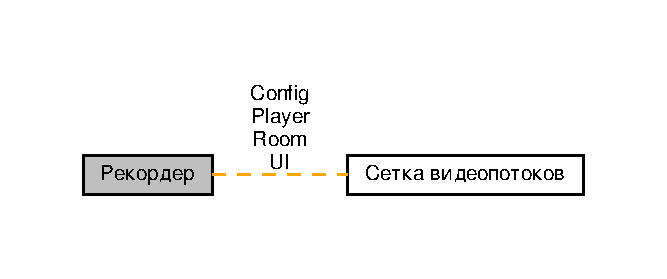
\includegraphics[width=320pt]{group__recorder}
\end{center}
\end{figure}
\subsection*{Классы}
\begin{DoxyCompactItemize}
\item 
class \hyperlink{class_config}{Config}
\begin{DoxyCompactList}\small\item\em The \hyperlink{class_config}{Config} class. \end{DoxyCompactList}\item 
class \hyperlink{class_player}{Player}
\begin{DoxyCompactList}\small\item\em The \hyperlink{class_player}{Player} class. \end{DoxyCompactList}\item 
class \hyperlink{class_recorder}{Recorder}
\begin{DoxyCompactList}\small\item\em Управляет процессом записи \end{DoxyCompactList}\item 
class \hyperlink{class_recording}{Recording}
\begin{DoxyCompactList}\small\item\em The \hyperlink{class_recording}{Recording} class. \end{DoxyCompactList}\item 
class \hyperlink{class_room}{Room}
\begin{DoxyCompactList}\small\item\em The \hyperlink{class_room}{Room} class. \end{DoxyCompactList}\item 
class \hyperlink{class_u_i}{UI}
\begin{DoxyCompactList}\small\item\em The \hyperlink{class_u_i}{UI} class. \end{DoxyCompactList}\end{DoxyCompactItemize}


\subsection{Подробное описание}
Выполняет запись видеопотоков, и их загрузку в Google Drive. 


\hypertarget{group__grid}{}\section{Сетка видеопотоков}
\label{group__grid}\index{Сетка видеопотоков@{Сетка видеопотоков}}


Отображает сетку изображений с камер  


Граф связей класса Сетка видеопотоков\+:\nopagebreak
\begin{figure}[H]
\begin{center}
\leavevmode
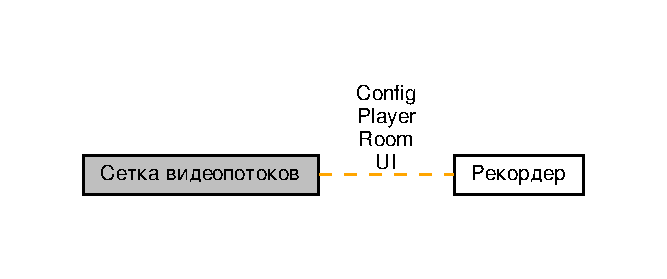
\includegraphics[width=320pt]{group__grid}
\end{center}
\end{figure}
\subsection*{Классы}
\begin{DoxyCompactItemize}
\item 
class \hyperlink{class_config}{Config}
\begin{DoxyCompactList}\small\item\em The \hyperlink{class_config}{Config} class. \end{DoxyCompactList}\item 
class \hyperlink{class_player}{Player}
\begin{DoxyCompactList}\small\item\em The \hyperlink{class_player}{Player} class. \end{DoxyCompactList}\item 
class \hyperlink{class_room}{Room}
\begin{DoxyCompactList}\small\item\em The \hyperlink{class_room}{Room} class. \end{DoxyCompactList}\item 
class \hyperlink{class_u_i}{UI}
\begin{DoxyCompactList}\small\item\em The \hyperlink{class_u_i}{UI} class. \end{DoxyCompactList}\end{DoxyCompactItemize}


\subsection{Подробное описание}
Отображает сетку изображений с камер 


\hypertarget{group__network__monitor}{}\section{Сетевой монитор}
\label{group__network__monitor}\index{Сетевой монитор@{Сетевой монитор}}


Выполняет ping камер и отображает график изменения значений для выбранной камеры  


\subsection*{Классы}
\begin{DoxyCompactItemize}
\item 
class \hyperlink{classnetwork__monitor_1_1_pinger}{network\+\_\+monitor.\+Pinger}
\begin{DoxyCompactList}\small\item\em Пингует камеры \end{DoxyCompactList}\end{DoxyCompactItemize}


\subsection{Подробное описание}
Выполняет ping камер и отображает график изменения значений для выбранной камеры 


\chapter{Пространства имен}
\hypertarget{namespacefrom-gsuite}{}\section{Пространство имен from-\/gsuite}
\label{namespacefrom-gsuite}\index{from-\/gsuite@{from-\/gsuite}}
\subsection*{Функции}
\begin{DoxyCompactItemize}
\item 
def \hyperlink{namespacefrom-gsuite_a431d5ae5f08baa594842e68180930f6c}{main} ()
\end{DoxyCompactItemize}
\subsection*{Переменные}
\begin{DoxyCompactItemize}
\item 
list \hyperlink{namespacefrom-gsuite_a359fb1aa3ebe4472fff6f682676e7dc0}{S\+C\+O\+P\+ES} = \mbox{[}\textquotesingle{}https\+://www.\+googleapis.\+com/auth/admin.\+directory.\+resource.\+calendar\textquotesingle{}\mbox{]}
\end{DoxyCompactItemize}


\subsection{Функции}
\mbox{\Hypertarget{namespacefrom-gsuite_a431d5ae5f08baa594842e68180930f6c}\label{namespacefrom-gsuite_a431d5ae5f08baa594842e68180930f6c}} 
\index{from-\/gsuite@{from-\/gsuite}!main@{main}}
\index{main@{main}!from-\/gsuite@{from-\/gsuite}}
\subsubsection{\texorpdfstring{main()}{main()}}
{\footnotesize\ttfamily def from-\/gsuite.\+main (\begin{DoxyParamCaption}{ }\end{DoxyParamCaption})}

\begin{DoxyVerb}Fetches cameras from GSuite and writes them to JSON file grouping by room 
\end{DoxyVerb}
 

\subsection{Переменные}
\mbox{\Hypertarget{namespacefrom-gsuite_a359fb1aa3ebe4472fff6f682676e7dc0}\label{namespacefrom-gsuite_a359fb1aa3ebe4472fff6f682676e7dc0}} 
\index{from-\/gsuite@{from-\/gsuite}!S\+C\+O\+P\+ES@{S\+C\+O\+P\+ES}}
\index{S\+C\+O\+P\+ES@{S\+C\+O\+P\+ES}!from-\/gsuite@{from-\/gsuite}}
\subsubsection{\texorpdfstring{S\+C\+O\+P\+ES}{SCOPES}}
{\footnotesize\ttfamily list from-\/gsuite.\+S\+C\+O\+P\+ES = \mbox{[}\textquotesingle{}https\+://www.\+googleapis.\+com/auth/admin.\+directory.\+resource.\+calendar\textquotesingle{}\mbox{]}}


\hypertarget{namespacegpio}{}\section{Пространство имен gpio}
\label{namespacegpio}\index{gpio@{gpio}}
\subsection*{Функции}
\begin{DoxyCompactItemize}
\item 
def \hyperlink{namespacegpio_a163967890b998f0910bb0cefc45939ab}{keypress} (key)
\item 
def \hyperlink{namespacegpio_a3d6472f268230baafcc5895596b07a6a}{stop\+\_\+cb} (channel=0)
\item 
def \hyperlink{namespacegpio_a29bb86ae5be5d1d6f4f2e8783480a8cd}{rec\+\_\+cb} (channel=0)
\item 
def \hyperlink{namespacegpio_a67087cfb10312de7d9b64c388777585f}{menu\+\_\+cb} (channel=0)
\item 
def \hyperlink{namespacegpio_ae76663bf79b1124596595094a9a95e5a}{main} ()
\end{DoxyCompactItemize}
\subsection*{Переменные}
\begin{DoxyCompactItemize}
\item 
int \hyperlink{namespacegpio_a00bc49404c7d994457664d6352bb2779}{stop} = 12
\item 
int \hyperlink{namespacegpio_ac4b0388fe69e716c5162432e3cdb535e}{rec} = 11
\item 
int \hyperlink{namespacegpio_a6f3cdec53dcabbe77f454382ef596f33}{menu} = 18
\item 
string \hyperlink{namespacegpio_acdd7abc8e2ded2f119524bc5e42af82e}{key\+\_\+r} = \char`\"{}key R \char`\"{}
\item 
string \hyperlink{namespacegpio_aab8c27a0b381c11af8ed5c638d612456}{key\+\_\+s} = \char`\"{}key S \char`\"{}
\item 
string \hyperlink{namespacegpio_af7fb6ee836b3b623fee0a157b4084380}{key\+\_\+m} = \char`\"{}key M \char`\"{}
\end{DoxyCompactItemize}


\subsection{Функции}
\mbox{\Hypertarget{namespacegpio_a163967890b998f0910bb0cefc45939ab}\label{namespacegpio_a163967890b998f0910bb0cefc45939ab}} 
\index{gpio@{gpio}!keypress@{keypress}}
\index{keypress@{keypress}!gpio@{gpio}}
\subsubsection{\texorpdfstring{keypress()}{keypress()}}
{\footnotesize\ttfamily def gpio.\+keypress (\begin{DoxyParamCaption}\item[{}]{key }\end{DoxyParamCaption})}

\mbox{\Hypertarget{namespacegpio_ae76663bf79b1124596595094a9a95e5a}\label{namespacegpio_ae76663bf79b1124596595094a9a95e5a}} 
\index{gpio@{gpio}!main@{main}}
\index{main@{main}!gpio@{gpio}}
\subsubsection{\texorpdfstring{main()}{main()}}
{\footnotesize\ttfamily def gpio.\+main (\begin{DoxyParamCaption}{ }\end{DoxyParamCaption})}

Граф вызовов\+:\nopagebreak
\begin{figure}[H]
\begin{center}
\leavevmode
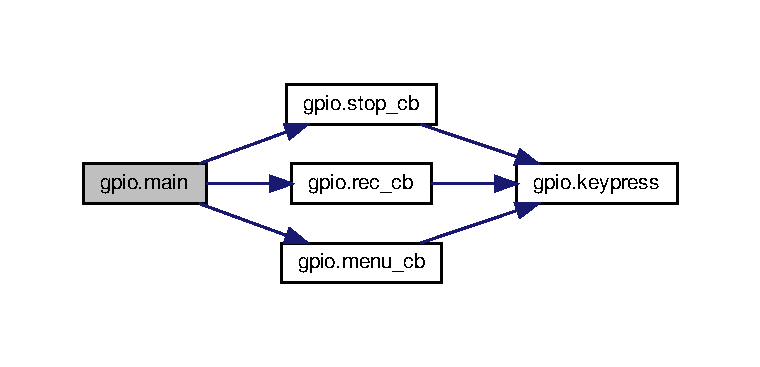
\includegraphics[width=350pt]{namespacegpio_ae76663bf79b1124596595094a9a95e5a_cgraph}
\end{center}
\end{figure}
\mbox{\Hypertarget{namespacegpio_a67087cfb10312de7d9b64c388777585f}\label{namespacegpio_a67087cfb10312de7d9b64c388777585f}} 
\index{gpio@{gpio}!menu\+\_\+cb@{menu\+\_\+cb}}
\index{menu\+\_\+cb@{menu\+\_\+cb}!gpio@{gpio}}
\subsubsection{\texorpdfstring{menu\+\_\+cb()}{menu\_cb()}}
{\footnotesize\ttfamily def gpio.\+menu\+\_\+cb (\begin{DoxyParamCaption}\item[{}]{channel = {\ttfamily 0} }\end{DoxyParamCaption})}

Граф вызовов\+:\nopagebreak
\begin{figure}[H]
\begin{center}
\leavevmode
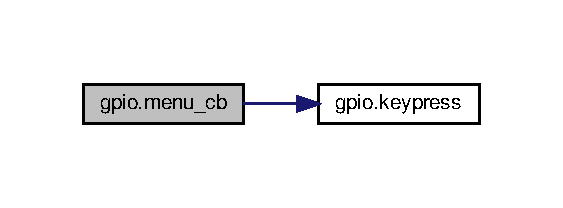
\includegraphics[width=270pt]{namespacegpio_a67087cfb10312de7d9b64c388777585f_cgraph}
\end{center}
\end{figure}
\mbox{\Hypertarget{namespacegpio_a29bb86ae5be5d1d6f4f2e8783480a8cd}\label{namespacegpio_a29bb86ae5be5d1d6f4f2e8783480a8cd}} 
\index{gpio@{gpio}!rec\+\_\+cb@{rec\+\_\+cb}}
\index{rec\+\_\+cb@{rec\+\_\+cb}!gpio@{gpio}}
\subsubsection{\texorpdfstring{rec\+\_\+cb()}{rec\_cb()}}
{\footnotesize\ttfamily def gpio.\+rec\+\_\+cb (\begin{DoxyParamCaption}\item[{}]{channel = {\ttfamily 0} }\end{DoxyParamCaption})}

Граф вызовов\+:\nopagebreak
\begin{figure}[H]
\begin{center}
\leavevmode
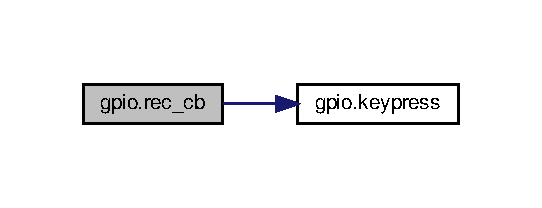
\includegraphics[width=260pt]{namespacegpio_a29bb86ae5be5d1d6f4f2e8783480a8cd_cgraph}
\end{center}
\end{figure}
\mbox{\Hypertarget{namespacegpio_a3d6472f268230baafcc5895596b07a6a}\label{namespacegpio_a3d6472f268230baafcc5895596b07a6a}} 
\index{gpio@{gpio}!stop\+\_\+cb@{stop\+\_\+cb}}
\index{stop\+\_\+cb@{stop\+\_\+cb}!gpio@{gpio}}
\subsubsection{\texorpdfstring{stop\+\_\+cb()}{stop\_cb()}}
{\footnotesize\ttfamily def gpio.\+stop\+\_\+cb (\begin{DoxyParamCaption}\item[{}]{channel = {\ttfamily 0} }\end{DoxyParamCaption})}

Граф вызовов\+:\nopagebreak
\begin{figure}[H]
\begin{center}
\leavevmode
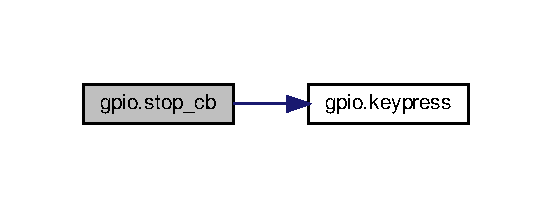
\includegraphics[width=265pt]{namespacegpio_a3d6472f268230baafcc5895596b07a6a_cgraph}
\end{center}
\end{figure}


\subsection{Переменные}
\mbox{\Hypertarget{namespacegpio_af7fb6ee836b3b623fee0a157b4084380}\label{namespacegpio_af7fb6ee836b3b623fee0a157b4084380}} 
\index{gpio@{gpio}!key\+\_\+m@{key\+\_\+m}}
\index{key\+\_\+m@{key\+\_\+m}!gpio@{gpio}}
\subsubsection{\texorpdfstring{key\+\_\+m}{key\_m}}
{\footnotesize\ttfamily string gpio.\+key\+\_\+m = \char`\"{}key M \char`\"{}}

\mbox{\Hypertarget{namespacegpio_acdd7abc8e2ded2f119524bc5e42af82e}\label{namespacegpio_acdd7abc8e2ded2f119524bc5e42af82e}} 
\index{gpio@{gpio}!key\+\_\+r@{key\+\_\+r}}
\index{key\+\_\+r@{key\+\_\+r}!gpio@{gpio}}
\subsubsection{\texorpdfstring{key\+\_\+r}{key\_r}}
{\footnotesize\ttfamily string gpio.\+key\+\_\+r = \char`\"{}key R \char`\"{}}

\mbox{\Hypertarget{namespacegpio_aab8c27a0b381c11af8ed5c638d612456}\label{namespacegpio_aab8c27a0b381c11af8ed5c638d612456}} 
\index{gpio@{gpio}!key\+\_\+s@{key\+\_\+s}}
\index{key\+\_\+s@{key\+\_\+s}!gpio@{gpio}}
\subsubsection{\texorpdfstring{key\+\_\+s}{key\_s}}
{\footnotesize\ttfamily string gpio.\+key\+\_\+s = \char`\"{}key S \char`\"{}}

\mbox{\Hypertarget{namespacegpio_a6f3cdec53dcabbe77f454382ef596f33}\label{namespacegpio_a6f3cdec53dcabbe77f454382ef596f33}} 
\index{gpio@{gpio}!menu@{menu}}
\index{menu@{menu}!gpio@{gpio}}
\subsubsection{\texorpdfstring{menu}{menu}}
{\footnotesize\ttfamily int gpio.\+menu = 18}

\mbox{\Hypertarget{namespacegpio_ac4b0388fe69e716c5162432e3cdb535e}\label{namespacegpio_ac4b0388fe69e716c5162432e3cdb535e}} 
\index{gpio@{gpio}!rec@{rec}}
\index{rec@{rec}!gpio@{gpio}}
\subsubsection{\texorpdfstring{rec}{rec}}
{\footnotesize\ttfamily int gpio.\+rec = 11}

\mbox{\Hypertarget{namespacegpio_a00bc49404c7d994457664d6352bb2779}\label{namespacegpio_a00bc49404c7d994457664d6352bb2779}} 
\index{gpio@{gpio}!stop@{stop}}
\index{stop@{stop}!gpio@{gpio}}
\subsubsection{\texorpdfstring{stop}{stop}}
{\footnotesize\ttfamily int gpio.\+stop = 12}


\hypertarget{namespacenetwork__monitor}{}\section{Пространство имен network\+\_\+monitor}
\label{namespacenetwork__monitor}\index{network\+\_\+monitor@{network\+\_\+monitor}}
\subsection*{Классы}
\begin{DoxyCompactItemize}
\item 
class \hyperlink{classnetwork__monitor_1_1_camera}{Camera}
\item 
class \hyperlink{classnetwork__monitor_1_1_grapher}{Grapher}
\item 
class \hyperlink{classnetwork__monitor_1_1_pinger}{Pinger}
\begin{DoxyCompactList}\small\item\em Пингует камеры \end{DoxyCompactList}\item 
class \hyperlink{classnetwork__monitor_1_1_u_i_graph}{U\+I\+Graph}
\item 
class \hyperlink{classnetwork__monitor_1_1_u_i_menu}{U\+I\+Menu}
\end{DoxyCompactItemize}
\subsection*{Функции}
\begin{DoxyCompactItemize}
\item 
def \hyperlink{namespacenetwork__monitor_aa615228bd6f33e03eb168421f8980368}{run\+Ping} ()
\end{DoxyCompactItemize}
\subsection*{Переменные}
\begin{DoxyCompactItemize}
\item 
dictionary \hyperlink{namespacenetwork__monitor_a58f207986e588fcaab74394ee1cf1bcb}{adresses}
\item 
\hyperlink{namespacenetwork__monitor_adbe4adbd468aaae0ca471744f30fa1f6}{app} = Qt\+Widgets.\+Q\+Application(\mbox{[}$\,$\mbox{]})
\item 
\hyperlink{namespacenetwork__monitor_ab8b736e67d7a9e580ef5b8ee4fe938f3}{menu} = \hyperlink{classnetwork__monitor_1_1_u_i_menu}{U\+I\+Menu}()
\item 
\hyperlink{namespacenetwork__monitor_aecaa32d63f4a4b3e0716b8fd40b8fb18}{stylesheet} = open(\char`\"{}../ui/stylesheet.\+css\char`\"{}, \char`\"{}r\char`\"{})
\item 
\hyperlink{namespacenetwork__monitor_aab66b1b4dd31ec48a9682731a2c7bff0}{display0} = Qt\+Widgets.\+Q\+Desktop\+Widget().screen\+Geometry(0)
\item 
\hyperlink{namespacenetwork__monitor_a699d5e9a412cebae671b9cd40b722391}{graph} = \hyperlink{classnetwork__monitor_1_1_u_i_graph}{U\+I\+Graph}()
\item 
\hyperlink{namespacenetwork__monitor_a37cbe75c4a7a0a69b30c0137312e181d}{display1} = Qt\+Widgets.\+Q\+Desktop\+Widget().screen\+Geometry(1)
\item 
\hyperlink{namespacenetwork__monitor_af816a5bcf89d9423a24881c39b602f90}{widget} = graph.\+find\+Child(pg.\+Plot\+Widget, \char`\"{}plotwidget\char`\"{})
\item 
\hyperlink{namespacenetwork__monitor_a26e25ec561afa4ed83eebb64d67c1b14}{plot} = widget.\+get\+Plot\+Item()
\item 
\hyperlink{namespacenetwork__monitor_a335a52bfad31ee0a6d975d8cb9e6db82}{right\+Axis} = plot.\+get\+Axis(\textquotesingle{}right\textquotesingle{})
\item 
\hyperlink{namespacenetwork__monitor_ad712067b9115dc6d60b0ad48899312d0}{left\+Axis} = plot.\+get\+Axis(\textquotesingle{}left\textquotesingle{})
\item 
dictionary \hyperlink{namespacenetwork__monitor_a7a1dfe61bcb6dea8bb5e51d87cfa6674}{label\+Style} = \{\textquotesingle{}color\textquotesingle{}\+: \textquotesingle{}\#F\+FF\textquotesingle{}, \textquotesingle{}\hyperlink{namespacenetwork__monitor_a3a49c4c8811caddc06b48cb72517bf6a}{font}-\/size\textquotesingle{}\+: \textquotesingle{}20pt\textquotesingle{}\}
\item 
\hyperlink{namespacenetwork__monitor_a093c6a470ae8f02c3ab41f344841d7b4}{units}
\item 
\hyperlink{namespacenetwork__monitor_a3a49c4c8811caddc06b48cb72517bf6a}{font} = Q\+Font()
\item 
\hyperlink{namespacenetwork__monitor_ab5dc49bb32143d840b5617593019b6cc}{tick\+Font}
\item 
\hyperlink{namespacenetwork__monitor_aa6307605f5261f2cc1985c18b1d6b525}{x}
\item 
\hyperlink{namespacenetwork__monitor_a21b2d9df8eef39c146e4d33a4d3ac153}{True}
\item 
\hyperlink{namespacenetwork__monitor_a3d4b2bbe9932d5f533511dd894a99987}{y}
\item 
\hyperlink{namespacenetwork__monitor_a0217c896f3b1258aa8de32cf83f58221}{alpha}
\item 
\hyperlink{namespacenetwork__monitor_a6caf9d5fe8492a62de30cc09eb3d6ee0}{grapher} = \hyperlink{classnetwork__monitor_1_1_grapher}{Grapher}(\hyperlink{namespacenetwork__monitor_a26e25ec561afa4ed83eebb64d67c1b14}{plot})
\item 
list \hyperlink{namespacenetwork__monitor_a7033c08f9dae3f4784ace432524d7c3d}{cams} = \mbox{[}$\,$\mbox{]}
\item 
int \hyperlink{namespacenetwork__monitor_acbaeef9dd38caeac7bfb4ce5cc555a68}{i} = 0
\item 
\hyperlink{namespacenetwork__monitor_a068b20f337cc6bb4d8f773203ba1eb72}{button} = menu.\+find\+Child(Qt\+Widgets.\+Q\+Push\+Button, \char`\"{}b\char`\"{} + str(\hyperlink{namespacenetwork__monitor_acbaeef9dd38caeac7bfb4ce5cc555a68}{i}))
\item 
\hyperlink{namespacenetwork__monitor_a581e75b195d137edaf37a10c8f54f10b}{label} = menu.\+find\+Child(Qt\+Widgets.\+Q\+Label, \char`\"{}l\char`\"{} + str(\hyperlink{namespacenetwork__monitor_acbaeef9dd38caeac7bfb4ce5cc555a68}{i}))
\item 
\hyperlink{namespacenetwork__monitor_a1642786c603ba143d757e407619d4a18}{camera} = \hyperlink{classnetwork__monitor_1_1_camera}{Camera}(\hyperlink{namespacenetwork__monitor_a58f207986e588fcaab74394ee1cf1bcb}{adresses}\mbox{[}c\mbox{]}, \hyperlink{namespacenetwork__monitor_a068b20f337cc6bb4d8f773203ba1eb72}{button}, \hyperlink{namespacenetwork__monitor_a581e75b195d137edaf37a10c8f54f10b}{label}, \hyperlink{namespacenetwork__monitor_a6caf9d5fe8492a62de30cc09eb3d6ee0}{grapher})
\item 
\hyperlink{namespacenetwork__monitor_af27fb18157e68ae57798c807d9a7ee63}{threadpool} = Q\+Thread\+Pool()
\item 
\hyperlink{namespacenetwork__monitor_a6b419aa619e07e27f109ac81f356fbeb}{ping\+Timer} = Q\+Timer()
\item 
\hyperlink{namespacenetwork__monitor_ad064e389b1b0120cadea8ef9d463f2da}{pinger} = \hyperlink{classnetwork__monitor_1_1_pinger}{Pinger}(\hyperlink{namespacenetwork__monitor_a7033c08f9dae3f4784ace432524d7c3d}{cams})
\end{DoxyCompactItemize}


\subsection{Функции}
\mbox{\Hypertarget{namespacenetwork__monitor_aa615228bd6f33e03eb168421f8980368}\label{namespacenetwork__monitor_aa615228bd6f33e03eb168421f8980368}} 
\index{network\+\_\+monitor@{network\+\_\+monitor}!run\+Ping@{run\+Ping}}
\index{run\+Ping@{run\+Ping}!network\+\_\+monitor@{network\+\_\+monitor}}
\subsubsection{\texorpdfstring{run\+Ping()}{runPing()}}
{\footnotesize\ttfamily def network\+\_\+monitor.\+run\+Ping (\begin{DoxyParamCaption}{ }\end{DoxyParamCaption})}



\subsection{Переменные}
\mbox{\Hypertarget{namespacenetwork__monitor_a58f207986e588fcaab74394ee1cf1bcb}\label{namespacenetwork__monitor_a58f207986e588fcaab74394ee1cf1bcb}} 
\index{network\+\_\+monitor@{network\+\_\+monitor}!adresses@{adresses}}
\index{adresses@{adresses}!network\+\_\+monitor@{network\+\_\+monitor}}
\subsubsection{\texorpdfstring{adresses}{adresses}}
{\footnotesize\ttfamily dictionary network\+\_\+monitor.\+adresses}

{\bfseries Инициализатор}
\begin{DoxyCode}
1 =  \{
2     \textcolor{stringliteral}{'51'}: \textcolor{stringliteral}{'172.18.200.51'},
3     \textcolor{stringliteral}{'52'}: \textcolor{stringliteral}{'172.18.200.52'},
4     \textcolor{stringliteral}{'53'}: \textcolor{stringliteral}{'172.18.200.53'},
5     \textcolor{stringliteral}{'54'}: \textcolor{stringliteral}{'172.18.200.54'},
6     \textcolor{stringliteral}{'55'}: \textcolor{stringliteral}{'172.18.200.55'},
7     \textcolor{stringliteral}{'56'}: \textcolor{stringliteral}{'172.18.200.56'},
8     \textcolor{stringliteral}{'30'}: \textcolor{stringliteral}{'172.18.199.30'},
9     \textcolor{stringliteral}{'32'}: \textcolor{stringliteral}{'172.18.199.32'},
10     \textcolor{stringliteral}{'42'}: \textcolor{stringliteral}{'192.168.15.42'},   
11 \}
\end{DoxyCode}
\mbox{\Hypertarget{namespacenetwork__monitor_a0217c896f3b1258aa8de32cf83f58221}\label{namespacenetwork__monitor_a0217c896f3b1258aa8de32cf83f58221}} 
\index{network\+\_\+monitor@{network\+\_\+monitor}!alpha@{alpha}}
\index{alpha@{alpha}!network\+\_\+monitor@{network\+\_\+monitor}}
\subsubsection{\texorpdfstring{alpha}{alpha}}
{\footnotesize\ttfamily network\+\_\+monitor.\+alpha}

\mbox{\Hypertarget{namespacenetwork__monitor_adbe4adbd468aaae0ca471744f30fa1f6}\label{namespacenetwork__monitor_adbe4adbd468aaae0ca471744f30fa1f6}} 
\index{network\+\_\+monitor@{network\+\_\+monitor}!app@{app}}
\index{app@{app}!network\+\_\+monitor@{network\+\_\+monitor}}
\subsubsection{\texorpdfstring{app}{app}}
{\footnotesize\ttfamily network\+\_\+monitor.\+app = Qt\+Widgets.\+Q\+Application(\mbox{[}$\,$\mbox{]})}

\mbox{\Hypertarget{namespacenetwork__monitor_a068b20f337cc6bb4d8f773203ba1eb72}\label{namespacenetwork__monitor_a068b20f337cc6bb4d8f773203ba1eb72}} 
\index{network\+\_\+monitor@{network\+\_\+monitor}!button@{button}}
\index{button@{button}!network\+\_\+monitor@{network\+\_\+monitor}}
\subsubsection{\texorpdfstring{button}{button}}
{\footnotesize\ttfamily network\+\_\+monitor.\+button = menu.\+find\+Child(Qt\+Widgets.\+Q\+Push\+Button, \char`\"{}b\char`\"{} + str(\hyperlink{namespacenetwork__monitor_acbaeef9dd38caeac7bfb4ce5cc555a68}{i}))}

\mbox{\Hypertarget{namespacenetwork__monitor_a1642786c603ba143d757e407619d4a18}\label{namespacenetwork__monitor_a1642786c603ba143d757e407619d4a18}} 
\index{network\+\_\+monitor@{network\+\_\+monitor}!camera@{camera}}
\index{camera@{camera}!network\+\_\+monitor@{network\+\_\+monitor}}
\subsubsection{\texorpdfstring{camera}{camera}}
{\footnotesize\ttfamily network\+\_\+monitor.\+camera = \hyperlink{classnetwork__monitor_1_1_camera}{Camera}(\hyperlink{namespacenetwork__monitor_a58f207986e588fcaab74394ee1cf1bcb}{adresses}\mbox{[}c\mbox{]}, \hyperlink{namespacenetwork__monitor_a068b20f337cc6bb4d8f773203ba1eb72}{button}, \hyperlink{namespacenetwork__monitor_a581e75b195d137edaf37a10c8f54f10b}{label}, \hyperlink{namespacenetwork__monitor_a6caf9d5fe8492a62de30cc09eb3d6ee0}{grapher})}

\mbox{\Hypertarget{namespacenetwork__monitor_a7033c08f9dae3f4784ace432524d7c3d}\label{namespacenetwork__monitor_a7033c08f9dae3f4784ace432524d7c3d}} 
\index{network\+\_\+monitor@{network\+\_\+monitor}!cams@{cams}}
\index{cams@{cams}!network\+\_\+monitor@{network\+\_\+monitor}}
\subsubsection{\texorpdfstring{cams}{cams}}
{\footnotesize\ttfamily list network\+\_\+monitor.\+cams = \mbox{[}$\,$\mbox{]}}

\mbox{\Hypertarget{namespacenetwork__monitor_aab66b1b4dd31ec48a9682731a2c7bff0}\label{namespacenetwork__monitor_aab66b1b4dd31ec48a9682731a2c7bff0}} 
\index{network\+\_\+monitor@{network\+\_\+monitor}!display0@{display0}}
\index{display0@{display0}!network\+\_\+monitor@{network\+\_\+monitor}}
\subsubsection{\texorpdfstring{display0}{display0}}
{\footnotesize\ttfamily network\+\_\+monitor.\+display0 = Qt\+Widgets.\+Q\+Desktop\+Widget().screen\+Geometry(0)}

\mbox{\Hypertarget{namespacenetwork__monitor_a37cbe75c4a7a0a69b30c0137312e181d}\label{namespacenetwork__monitor_a37cbe75c4a7a0a69b30c0137312e181d}} 
\index{network\+\_\+monitor@{network\+\_\+monitor}!display1@{display1}}
\index{display1@{display1}!network\+\_\+monitor@{network\+\_\+monitor}}
\subsubsection{\texorpdfstring{display1}{display1}}
{\footnotesize\ttfamily network\+\_\+monitor.\+display1 = Qt\+Widgets.\+Q\+Desktop\+Widget().screen\+Geometry(1)}

\mbox{\Hypertarget{namespacenetwork__monitor_a3a49c4c8811caddc06b48cb72517bf6a}\label{namespacenetwork__monitor_a3a49c4c8811caddc06b48cb72517bf6a}} 
\index{network\+\_\+monitor@{network\+\_\+monitor}!font@{font}}
\index{font@{font}!network\+\_\+monitor@{network\+\_\+monitor}}
\subsubsection{\texorpdfstring{font}{font}}
{\footnotesize\ttfamily network\+\_\+monitor.\+font = Q\+Font()}

\mbox{\Hypertarget{namespacenetwork__monitor_a699d5e9a412cebae671b9cd40b722391}\label{namespacenetwork__monitor_a699d5e9a412cebae671b9cd40b722391}} 
\index{network\+\_\+monitor@{network\+\_\+monitor}!graph@{graph}}
\index{graph@{graph}!network\+\_\+monitor@{network\+\_\+monitor}}
\subsubsection{\texorpdfstring{graph}{graph}}
{\footnotesize\ttfamily network\+\_\+monitor.\+graph = \hyperlink{classnetwork__monitor_1_1_u_i_graph}{U\+I\+Graph}()}

\mbox{\Hypertarget{namespacenetwork__monitor_a6caf9d5fe8492a62de30cc09eb3d6ee0}\label{namespacenetwork__monitor_a6caf9d5fe8492a62de30cc09eb3d6ee0}} 
\index{network\+\_\+monitor@{network\+\_\+monitor}!grapher@{grapher}}
\index{grapher@{grapher}!network\+\_\+monitor@{network\+\_\+monitor}}
\subsubsection{\texorpdfstring{grapher}{grapher}}
{\footnotesize\ttfamily network\+\_\+monitor.\+grapher = \hyperlink{classnetwork__monitor_1_1_grapher}{Grapher}(\hyperlink{namespacenetwork__monitor_a26e25ec561afa4ed83eebb64d67c1b14}{plot})}

\mbox{\Hypertarget{namespacenetwork__monitor_acbaeef9dd38caeac7bfb4ce5cc555a68}\label{namespacenetwork__monitor_acbaeef9dd38caeac7bfb4ce5cc555a68}} 
\index{network\+\_\+monitor@{network\+\_\+monitor}!i@{i}}
\index{i@{i}!network\+\_\+monitor@{network\+\_\+monitor}}
\subsubsection{\texorpdfstring{i}{i}}
{\footnotesize\ttfamily int network\+\_\+monitor.\+i = 0}

\mbox{\Hypertarget{namespacenetwork__monitor_a581e75b195d137edaf37a10c8f54f10b}\label{namespacenetwork__monitor_a581e75b195d137edaf37a10c8f54f10b}} 
\index{network\+\_\+monitor@{network\+\_\+monitor}!label@{label}}
\index{label@{label}!network\+\_\+monitor@{network\+\_\+monitor}}
\subsubsection{\texorpdfstring{label}{label}}
{\footnotesize\ttfamily network\+\_\+monitor.\+label = menu.\+find\+Child(Qt\+Widgets.\+Q\+Label, \char`\"{}l\char`\"{} + str(\hyperlink{namespacenetwork__monitor_acbaeef9dd38caeac7bfb4ce5cc555a68}{i}))}

\mbox{\Hypertarget{namespacenetwork__monitor_a7a1dfe61bcb6dea8bb5e51d87cfa6674}\label{namespacenetwork__monitor_a7a1dfe61bcb6dea8bb5e51d87cfa6674}} 
\index{network\+\_\+monitor@{network\+\_\+monitor}!label\+Style@{label\+Style}}
\index{label\+Style@{label\+Style}!network\+\_\+monitor@{network\+\_\+monitor}}
\subsubsection{\texorpdfstring{label\+Style}{labelStyle}}
{\footnotesize\ttfamily dictionary network\+\_\+monitor.\+label\+Style = \{\textquotesingle{}color\textquotesingle{}\+: \textquotesingle{}\#F\+FF\textquotesingle{}, \textquotesingle{}\hyperlink{namespacenetwork__monitor_a3a49c4c8811caddc06b48cb72517bf6a}{font}-\/size\textquotesingle{}\+: \textquotesingle{}20pt\textquotesingle{}\}}

\mbox{\Hypertarget{namespacenetwork__monitor_ad712067b9115dc6d60b0ad48899312d0}\label{namespacenetwork__monitor_ad712067b9115dc6d60b0ad48899312d0}} 
\index{network\+\_\+monitor@{network\+\_\+monitor}!left\+Axis@{left\+Axis}}
\index{left\+Axis@{left\+Axis}!network\+\_\+monitor@{network\+\_\+monitor}}
\subsubsection{\texorpdfstring{left\+Axis}{leftAxis}}
{\footnotesize\ttfamily network\+\_\+monitor.\+left\+Axis = plot.\+get\+Axis(\textquotesingle{}left\textquotesingle{})}

\mbox{\Hypertarget{namespacenetwork__monitor_ab8b736e67d7a9e580ef5b8ee4fe938f3}\label{namespacenetwork__monitor_ab8b736e67d7a9e580ef5b8ee4fe938f3}} 
\index{network\+\_\+monitor@{network\+\_\+monitor}!menu@{menu}}
\index{menu@{menu}!network\+\_\+monitor@{network\+\_\+monitor}}
\subsubsection{\texorpdfstring{menu}{menu}}
{\footnotesize\ttfamily network\+\_\+monitor.\+menu = \hyperlink{classnetwork__monitor_1_1_u_i_menu}{U\+I\+Menu}()}

\mbox{\Hypertarget{namespacenetwork__monitor_ad064e389b1b0120cadea8ef9d463f2da}\label{namespacenetwork__monitor_ad064e389b1b0120cadea8ef9d463f2da}} 
\index{network\+\_\+monitor@{network\+\_\+monitor}!pinger@{pinger}}
\index{pinger@{pinger}!network\+\_\+monitor@{network\+\_\+monitor}}
\subsubsection{\texorpdfstring{pinger}{pinger}}
{\footnotesize\ttfamily network\+\_\+monitor.\+pinger = \hyperlink{classnetwork__monitor_1_1_pinger}{Pinger}(\hyperlink{namespacenetwork__monitor_a7033c08f9dae3f4784ace432524d7c3d}{cams})}

\mbox{\Hypertarget{namespacenetwork__monitor_a6b419aa619e07e27f109ac81f356fbeb}\label{namespacenetwork__monitor_a6b419aa619e07e27f109ac81f356fbeb}} 
\index{network\+\_\+monitor@{network\+\_\+monitor}!ping\+Timer@{ping\+Timer}}
\index{ping\+Timer@{ping\+Timer}!network\+\_\+monitor@{network\+\_\+monitor}}
\subsubsection{\texorpdfstring{ping\+Timer}{pingTimer}}
{\footnotesize\ttfamily network\+\_\+monitor.\+ping\+Timer = Q\+Timer()}

\mbox{\Hypertarget{namespacenetwork__monitor_a26e25ec561afa4ed83eebb64d67c1b14}\label{namespacenetwork__monitor_a26e25ec561afa4ed83eebb64d67c1b14}} 
\index{network\+\_\+monitor@{network\+\_\+monitor}!plot@{plot}}
\index{plot@{plot}!network\+\_\+monitor@{network\+\_\+monitor}}
\subsubsection{\texorpdfstring{plot}{plot}}
{\footnotesize\ttfamily network\+\_\+monitor.\+plot = widget.\+get\+Plot\+Item()}

\mbox{\Hypertarget{namespacenetwork__monitor_a335a52bfad31ee0a6d975d8cb9e6db82}\label{namespacenetwork__monitor_a335a52bfad31ee0a6d975d8cb9e6db82}} 
\index{network\+\_\+monitor@{network\+\_\+monitor}!right\+Axis@{right\+Axis}}
\index{right\+Axis@{right\+Axis}!network\+\_\+monitor@{network\+\_\+monitor}}
\subsubsection{\texorpdfstring{right\+Axis}{rightAxis}}
{\footnotesize\ttfamily network\+\_\+monitor.\+right\+Axis = plot.\+get\+Axis(\textquotesingle{}right\textquotesingle{})}

\mbox{\Hypertarget{namespacenetwork__monitor_aecaa32d63f4a4b3e0716b8fd40b8fb18}\label{namespacenetwork__monitor_aecaa32d63f4a4b3e0716b8fd40b8fb18}} 
\index{network\+\_\+monitor@{network\+\_\+monitor}!stylesheet@{stylesheet}}
\index{stylesheet@{stylesheet}!network\+\_\+monitor@{network\+\_\+monitor}}
\subsubsection{\texorpdfstring{stylesheet}{stylesheet}}
{\footnotesize\ttfamily network\+\_\+monitor.\+stylesheet = open(\char`\"{}../ui/stylesheet.\+css\char`\"{}, \char`\"{}r\char`\"{})}

\mbox{\Hypertarget{namespacenetwork__monitor_af27fb18157e68ae57798c807d9a7ee63}\label{namespacenetwork__monitor_af27fb18157e68ae57798c807d9a7ee63}} 
\index{network\+\_\+monitor@{network\+\_\+monitor}!threadpool@{threadpool}}
\index{threadpool@{threadpool}!network\+\_\+monitor@{network\+\_\+monitor}}
\subsubsection{\texorpdfstring{threadpool}{threadpool}}
{\footnotesize\ttfamily network\+\_\+monitor.\+threadpool = Q\+Thread\+Pool()}

\mbox{\Hypertarget{namespacenetwork__monitor_ab5dc49bb32143d840b5617593019b6cc}\label{namespacenetwork__monitor_ab5dc49bb32143d840b5617593019b6cc}} 
\index{network\+\_\+monitor@{network\+\_\+monitor}!tick\+Font@{tick\+Font}}
\index{tick\+Font@{tick\+Font}!network\+\_\+monitor@{network\+\_\+monitor}}
\subsubsection{\texorpdfstring{tick\+Font}{tickFont}}
{\footnotesize\ttfamily network\+\_\+monitor.\+tick\+Font}

\mbox{\Hypertarget{namespacenetwork__monitor_a21b2d9df8eef39c146e4d33a4d3ac153}\label{namespacenetwork__monitor_a21b2d9df8eef39c146e4d33a4d3ac153}} 
\index{network\+\_\+monitor@{network\+\_\+monitor}!True@{True}}
\index{True@{True}!network\+\_\+monitor@{network\+\_\+monitor}}
\subsubsection{\texorpdfstring{True}{True}}
{\footnotesize\ttfamily network\+\_\+monitor.\+True}

\mbox{\Hypertarget{namespacenetwork__monitor_a093c6a470ae8f02c3ab41f344841d7b4}\label{namespacenetwork__monitor_a093c6a470ae8f02c3ab41f344841d7b4}} 
\index{network\+\_\+monitor@{network\+\_\+monitor}!units@{units}}
\index{units@{units}!network\+\_\+monitor@{network\+\_\+monitor}}
\subsubsection{\texorpdfstring{units}{units}}
{\footnotesize\ttfamily network\+\_\+monitor.\+units}

\mbox{\Hypertarget{namespacenetwork__monitor_af816a5bcf89d9423a24881c39b602f90}\label{namespacenetwork__monitor_af816a5bcf89d9423a24881c39b602f90}} 
\index{network\+\_\+monitor@{network\+\_\+monitor}!widget@{widget}}
\index{widget@{widget}!network\+\_\+monitor@{network\+\_\+monitor}}
\subsubsection{\texorpdfstring{widget}{widget}}
{\footnotesize\ttfamily network\+\_\+monitor.\+widget = graph.\+find\+Child(pg.\+Plot\+Widget, \char`\"{}plotwidget\char`\"{})}

\mbox{\Hypertarget{namespacenetwork__monitor_aa6307605f5261f2cc1985c18b1d6b525}\label{namespacenetwork__monitor_aa6307605f5261f2cc1985c18b1d6b525}} 
\index{network\+\_\+monitor@{network\+\_\+monitor}!x@{x}}
\index{x@{x}!network\+\_\+monitor@{network\+\_\+monitor}}
\subsubsection{\texorpdfstring{x}{x}}
{\footnotesize\ttfamily network\+\_\+monitor.\+x}

\mbox{\Hypertarget{namespacenetwork__monitor_a3d4b2bbe9932d5f533511dd894a99987}\label{namespacenetwork__monitor_a3d4b2bbe9932d5f533511dd894a99987}} 
\index{network\+\_\+monitor@{network\+\_\+monitor}!y@{y}}
\index{y@{y}!network\+\_\+monitor@{network\+\_\+monitor}}
\subsubsection{\texorpdfstring{y}{y}}
{\footnotesize\ttfamily network\+\_\+monitor.\+y}


\hypertarget{namespacevideo-upload}{}\section{Пространство имен video-\/upload}
\label{namespacevideo-upload}\index{video-\/upload@{video-\/upload}}
\subsection*{Переменные}
\begin{DoxyCompactItemize}
\item 
\hyperlink{namespacevideo-upload_adb444a75aaa0c0e590807701931bafef}{parser} = argparse.\+Argument\+Parser(\char`\"{}Videofile name and location\char`\"{})
\item 
\hyperlink{namespacevideo-upload_a7febd43c5f8604092229ae1ccf261f0c}{help}
\item 
\hyperlink{namespacevideo-upload_a0aea8bad307fcc1764683855862406c5}{type}
\item 
\hyperlink{namespacevideo-upload_a9e790ab261c9413ed47dafe46c022063}{args} = parser.\+parse\+\_\+args()
\item 
string \hyperlink{namespacevideo-upload_a76e331163a34b55da69ecdf6ca084eab}{S\+C\+O\+P\+ES} = \textquotesingle{}https\+://www.\+googleapis.\+com/auth/drive.\+file\textquotesingle{}
\item 
\hyperlink{namespacevideo-upload_a1bbb99b1568829c7cb6af40564c671d3}{store} = file.\+Storage(\textquotesingle{}storage.\+json\textquotesingle{})
\item 
\hyperlink{namespacevideo-upload_a5c691a1aa9c397a8485738b164fbf511}{creds} = store.\+get()
\item 
\hyperlink{namespacevideo-upload_a7f676962b30f842d93805a11467d4404}{flow} = client.\+flow\+\_\+from\+\_\+clientsecrets(\textquotesingle{}client\+\_\+secret.\+json\textquotesingle{}, scope = \hyperlink{namespacevideo-upload_a76e331163a34b55da69ecdf6ca084eab}{S\+C\+O\+P\+ES})
\item 
\hyperlink{namespacevideo-upload_a70c1c74c0d69dbc8748f55e9678bd7e8}{D\+R\+I\+VE} = build(\textquotesingle{}drive\textquotesingle{}, \textquotesingle{}v3\textquotesingle{}, http = creds.\+authorize(Http()))
\item 
\hyperlink{namespacevideo-upload_a8f0c224b0d6326d66b6a471fb3ae06b7}{filename} = args.\+location + args.\+filename
\item 
dictionary \hyperlink{namespacevideo-upload_a078e77756bf147602ea81c2485e0b3ca}{metadata} = \{\textquotesingle{}name\textquotesingle{}\+: args.\+filename\}
\item 
\hyperlink{namespacevideo-upload_a98d77aa7929949660affdd840263f994}{res} = D\+R\+I\+V\+E.\+files().create(body = \hyperlink{namespacevideo-upload_a078e77756bf147602ea81c2485e0b3ca}{metadata}, media\+\_\+body = \hyperlink{namespacevideo-upload_a8f0c224b0d6326d66b6a471fb3ae06b7}{filename}).execute()
\end{DoxyCompactItemize}


\subsection{Переменные}
\mbox{\Hypertarget{namespacevideo-upload_a9e790ab261c9413ed47dafe46c022063}\label{namespacevideo-upload_a9e790ab261c9413ed47dafe46c022063}} 
\index{video-\/upload@{video-\/upload}!args@{args}}
\index{args@{args}!video-\/upload@{video-\/upload}}
\subsubsection{\texorpdfstring{args}{args}}
{\footnotesize\ttfamily video-\/upload.\+args = parser.\+parse\+\_\+args()}

\mbox{\Hypertarget{namespacevideo-upload_a5c691a1aa9c397a8485738b164fbf511}\label{namespacevideo-upload_a5c691a1aa9c397a8485738b164fbf511}} 
\index{video-\/upload@{video-\/upload}!creds@{creds}}
\index{creds@{creds}!video-\/upload@{video-\/upload}}
\subsubsection{\texorpdfstring{creds}{creds}}
{\footnotesize\ttfamily video-\/upload.\+creds = store.\+get()}

\mbox{\Hypertarget{namespacevideo-upload_a70c1c74c0d69dbc8748f55e9678bd7e8}\label{namespacevideo-upload_a70c1c74c0d69dbc8748f55e9678bd7e8}} 
\index{video-\/upload@{video-\/upload}!D\+R\+I\+VE@{D\+R\+I\+VE}}
\index{D\+R\+I\+VE@{D\+R\+I\+VE}!video-\/upload@{video-\/upload}}
\subsubsection{\texorpdfstring{D\+R\+I\+VE}{DRIVE}}
{\footnotesize\ttfamily video-\/upload.\+D\+R\+I\+VE = build(\textquotesingle{}drive\textquotesingle{}, \textquotesingle{}v3\textquotesingle{}, http = creds.\+authorize(Http()))}

\mbox{\Hypertarget{namespacevideo-upload_a8f0c224b0d6326d66b6a471fb3ae06b7}\label{namespacevideo-upload_a8f0c224b0d6326d66b6a471fb3ae06b7}} 
\index{video-\/upload@{video-\/upload}!filename@{filename}}
\index{filename@{filename}!video-\/upload@{video-\/upload}}
\subsubsection{\texorpdfstring{filename}{filename}}
{\footnotesize\ttfamily video-\/upload.\+filename = args.\+location + args.\+filename}

\mbox{\Hypertarget{namespacevideo-upload_a7f676962b30f842d93805a11467d4404}\label{namespacevideo-upload_a7f676962b30f842d93805a11467d4404}} 
\index{video-\/upload@{video-\/upload}!flow@{flow}}
\index{flow@{flow}!video-\/upload@{video-\/upload}}
\subsubsection{\texorpdfstring{flow}{flow}}
{\footnotesize\ttfamily video-\/upload.\+flow = client.\+flow\+\_\+from\+\_\+clientsecrets(\textquotesingle{}client\+\_\+secret.\+json\textquotesingle{}, scope = \hyperlink{namespacevideo-upload_a76e331163a34b55da69ecdf6ca084eab}{S\+C\+O\+P\+ES})}

\mbox{\Hypertarget{namespacevideo-upload_a7febd43c5f8604092229ae1ccf261f0c}\label{namespacevideo-upload_a7febd43c5f8604092229ae1ccf261f0c}} 
\index{video-\/upload@{video-\/upload}!help@{help}}
\index{help@{help}!video-\/upload@{video-\/upload}}
\subsubsection{\texorpdfstring{help}{help}}
{\footnotesize\ttfamily video-\/upload.\+help}

\mbox{\Hypertarget{namespacevideo-upload_a078e77756bf147602ea81c2485e0b3ca}\label{namespacevideo-upload_a078e77756bf147602ea81c2485e0b3ca}} 
\index{video-\/upload@{video-\/upload}!metadata@{metadata}}
\index{metadata@{metadata}!video-\/upload@{video-\/upload}}
\subsubsection{\texorpdfstring{metadata}{metadata}}
{\footnotesize\ttfamily dictionary video-\/upload.\+metadata = \{\textquotesingle{}name\textquotesingle{}\+: args.\+filename\}}

\mbox{\Hypertarget{namespacevideo-upload_adb444a75aaa0c0e590807701931bafef}\label{namespacevideo-upload_adb444a75aaa0c0e590807701931bafef}} 
\index{video-\/upload@{video-\/upload}!parser@{parser}}
\index{parser@{parser}!video-\/upload@{video-\/upload}}
\subsubsection{\texorpdfstring{parser}{parser}}
{\footnotesize\ttfamily video-\/upload.\+parser = argparse.\+Argument\+Parser(\char`\"{}Videofile name and location\char`\"{})}

\mbox{\Hypertarget{namespacevideo-upload_a98d77aa7929949660affdd840263f994}\label{namespacevideo-upload_a98d77aa7929949660affdd840263f994}} 
\index{video-\/upload@{video-\/upload}!res@{res}}
\index{res@{res}!video-\/upload@{video-\/upload}}
\subsubsection{\texorpdfstring{res}{res}}
{\footnotesize\ttfamily video-\/upload.\+res = D\+R\+I\+V\+E.\+files().create(body = \hyperlink{namespacevideo-upload_a078e77756bf147602ea81c2485e0b3ca}{metadata}, media\+\_\+body = \hyperlink{namespacevideo-upload_a8f0c224b0d6326d66b6a471fb3ae06b7}{filename}).execute()}

\mbox{\Hypertarget{namespacevideo-upload_a76e331163a34b55da69ecdf6ca084eab}\label{namespacevideo-upload_a76e331163a34b55da69ecdf6ca084eab}} 
\index{video-\/upload@{video-\/upload}!S\+C\+O\+P\+ES@{S\+C\+O\+P\+ES}}
\index{S\+C\+O\+P\+ES@{S\+C\+O\+P\+ES}!video-\/upload@{video-\/upload}}
\subsubsection{\texorpdfstring{S\+C\+O\+P\+ES}{SCOPES}}
{\footnotesize\ttfamily string video-\/upload.\+S\+C\+O\+P\+ES = \textquotesingle{}https\+://www.\+googleapis.\+com/auth/drive.\+file\textquotesingle{}}

\mbox{\Hypertarget{namespacevideo-upload_a1bbb99b1568829c7cb6af40564c671d3}\label{namespacevideo-upload_a1bbb99b1568829c7cb6af40564c671d3}} 
\index{video-\/upload@{video-\/upload}!store@{store}}
\index{store@{store}!video-\/upload@{video-\/upload}}
\subsubsection{\texorpdfstring{store}{store}}
{\footnotesize\ttfamily video-\/upload.\+store = file.\+Storage(\textquotesingle{}storage.\+json\textquotesingle{})}

\mbox{\Hypertarget{namespacevideo-upload_a0aea8bad307fcc1764683855862406c5}\label{namespacevideo-upload_a0aea8bad307fcc1764683855862406c5}} 
\index{video-\/upload@{video-\/upload}!type@{type}}
\index{type@{type}!video-\/upload@{video-\/upload}}
\subsubsection{\texorpdfstring{type}{type}}
{\footnotesize\ttfamily video-\/upload.\+type}


\chapter{Классы}
\hypertarget{struct_audio_source}{}\section{Структура Audio\+Source}
\label{struct_audio_source}\index{Audio\+Source@{Audio\+Source}}


{\ttfamily \#include $<$room.\+h$>$}

\subsection*{Открытые атрибуты}
\begin{DoxyCompactItemize}
\item 
string \hyperlink{struct_audio_source_ab4db8d8ad6e0552f565932b7b3f432ee}{name}
\item 
string \hyperlink{struct_audio_source_a462a95c3122f83138e524f2c26361a1c}{uri}
\end{DoxyCompactItemize}


\subsection{Данные класса}
\mbox{\Hypertarget{struct_audio_source_ab4db8d8ad6e0552f565932b7b3f432ee}\label{struct_audio_source_ab4db8d8ad6e0552f565932b7b3f432ee}} 
\index{Audio\+Source@{Audio\+Source}!name@{name}}
\index{name@{name}!Audio\+Source@{Audio\+Source}}
\subsubsection{\texorpdfstring{name}{name}}
{\footnotesize\ttfamily string Audio\+Source\+::name}

\mbox{\Hypertarget{struct_audio_source_a462a95c3122f83138e524f2c26361a1c}\label{struct_audio_source_a462a95c3122f83138e524f2c26361a1c}} 
\index{Audio\+Source@{Audio\+Source}!uri@{uri}}
\index{uri@{uri}!Audio\+Source@{Audio\+Source}}
\subsubsection{\texorpdfstring{uri}{uri}}
{\footnotesize\ttfamily string Audio\+Source\+::uri}



Объявления и описания членов структуры находятся в файле\+:\begin{DoxyCompactItemize}
\item 
/home/jetson/controlroom/\+Studio/\+Operator/\+Grid/include/\hyperlink{_operator_2_grid_2include_2room_8h}{room.\+h}\end{DoxyCompactItemize}

\hypertarget{classnetwork__monitor_1_1_camera}{}\section{Класс network\+\_\+monitor.\+Camera}
\label{classnetwork__monitor_1_1_camera}\index{network\+\_\+monitor.\+Camera@{network\+\_\+monitor.\+Camera}}
\subsection*{Открытые члены}
\begin{DoxyCompactItemize}
\item 
def \hyperlink{classnetwork__monitor_1_1_camera_a532428283b6b7737a01bdaf24989e8fe}{\+\_\+\+\_\+init\+\_\+\+\_\+} (self, \hyperlink{classnetwork__monitor_1_1_camera_a1bc250a15db245c87039d9984fe50b15}{ip}, \hyperlink{classnetwork__monitor_1_1_camera_ab51939018f21aebe68caa75c092d0098}{button}, \hyperlink{classnetwork__monitor_1_1_camera_afdb6d9fb249e5b2cc270e97572a40511}{label}, \hyperlink{classnetwork__monitor_1_1_camera_afdc20dd995418fb9a7c918ff41431ec0}{grapher})
\item 
def \hyperlink{classnetwork__monitor_1_1_camera_a6b175c56be99a6cb4ffcc058d878619b}{set\+Ping} (self, error, time)
\item 
def \hyperlink{classnetwork__monitor_1_1_camera_a2a22416b3e879c143b6e6d72034639c7}{draw\+Me} (self)
\end{DoxyCompactItemize}
\subsection*{Открытые атрибуты}
\begin{DoxyCompactItemize}
\item 
\hyperlink{classnetwork__monitor_1_1_camera_a1bc250a15db245c87039d9984fe50b15}{ip}
\item 
\hyperlink{classnetwork__monitor_1_1_camera_ab51939018f21aebe68caa75c092d0098}{button}
\item 
\hyperlink{classnetwork__monitor_1_1_camera_afdb6d9fb249e5b2cc270e97572a40511}{label}
\item 
\hyperlink{classnetwork__monitor_1_1_camera_afdc20dd995418fb9a7c918ff41431ec0}{grapher}
\item 
\hyperlink{classnetwork__monitor_1_1_camera_ae5f4e0501c0251f377ec26660c465e3b}{ping\+History}
\end{DoxyCompactItemize}


\subsection{Подробное описание}
\begin{DoxyVerb}Containes all camera information and ui objects\end{DoxyVerb}
 

\subsection{Конструктор(ы)}
\mbox{\Hypertarget{classnetwork__monitor_1_1_camera_a532428283b6b7737a01bdaf24989e8fe}\label{classnetwork__monitor_1_1_camera_a532428283b6b7737a01bdaf24989e8fe}} 
\index{network\+\_\+monitor\+::\+Camera@{network\+\_\+monitor\+::\+Camera}!\+\_\+\+\_\+init\+\_\+\+\_\+@{\+\_\+\+\_\+init\+\_\+\+\_\+}}
\index{\+\_\+\+\_\+init\+\_\+\+\_\+@{\+\_\+\+\_\+init\+\_\+\+\_\+}!network\+\_\+monitor\+::\+Camera@{network\+\_\+monitor\+::\+Camera}}
\subsubsection{\texorpdfstring{\+\_\+\+\_\+init\+\_\+\+\_\+()}{\_\_init\_\_()}}
{\footnotesize\ttfamily def network\+\_\+monitor.\+Camera.\+\_\+\+\_\+init\+\_\+\+\_\+ (\begin{DoxyParamCaption}\item[{}]{self,  }\item[{}]{ip,  }\item[{}]{button,  }\item[{}]{label,  }\item[{}]{grapher }\end{DoxyParamCaption})}



\subsection{Методы}
\mbox{\Hypertarget{classnetwork__monitor_1_1_camera_a2a22416b3e879c143b6e6d72034639c7}\label{classnetwork__monitor_1_1_camera_a2a22416b3e879c143b6e6d72034639c7}} 
\index{network\+\_\+monitor\+::\+Camera@{network\+\_\+monitor\+::\+Camera}!draw\+Me@{draw\+Me}}
\index{draw\+Me@{draw\+Me}!network\+\_\+monitor\+::\+Camera@{network\+\_\+monitor\+::\+Camera}}
\subsubsection{\texorpdfstring{draw\+Me()}{drawMe()}}
{\footnotesize\ttfamily def network\+\_\+monitor.\+Camera.\+draw\+Me (\begin{DoxyParamCaption}\item[{}]{self }\end{DoxyParamCaption})}

\mbox{\Hypertarget{classnetwork__monitor_1_1_camera_a6b175c56be99a6cb4ffcc058d878619b}\label{classnetwork__monitor_1_1_camera_a6b175c56be99a6cb4ffcc058d878619b}} 
\index{network\+\_\+monitor\+::\+Camera@{network\+\_\+monitor\+::\+Camera}!set\+Ping@{set\+Ping}}
\index{set\+Ping@{set\+Ping}!network\+\_\+monitor\+::\+Camera@{network\+\_\+monitor\+::\+Camera}}
\subsubsection{\texorpdfstring{set\+Ping()}{setPing()}}
{\footnotesize\ttfamily def network\+\_\+monitor.\+Camera.\+set\+Ping (\begin{DoxyParamCaption}\item[{}]{self,  }\item[{}]{error,  }\item[{}]{time }\end{DoxyParamCaption})}



\subsection{Данные класса}
\mbox{\Hypertarget{classnetwork__monitor_1_1_camera_ab51939018f21aebe68caa75c092d0098}\label{classnetwork__monitor_1_1_camera_ab51939018f21aebe68caa75c092d0098}} 
\index{network\+\_\+monitor\+::\+Camera@{network\+\_\+monitor\+::\+Camera}!button@{button}}
\index{button@{button}!network\+\_\+monitor\+::\+Camera@{network\+\_\+monitor\+::\+Camera}}
\subsubsection{\texorpdfstring{button}{button}}
{\footnotesize\ttfamily network\+\_\+monitor.\+Camera.\+button}

\mbox{\Hypertarget{classnetwork__monitor_1_1_camera_afdc20dd995418fb9a7c918ff41431ec0}\label{classnetwork__monitor_1_1_camera_afdc20dd995418fb9a7c918ff41431ec0}} 
\index{network\+\_\+monitor\+::\+Camera@{network\+\_\+monitor\+::\+Camera}!grapher@{grapher}}
\index{grapher@{grapher}!network\+\_\+monitor\+::\+Camera@{network\+\_\+monitor\+::\+Camera}}
\subsubsection{\texorpdfstring{grapher}{grapher}}
{\footnotesize\ttfamily network\+\_\+monitor.\+Camera.\+grapher}

\mbox{\Hypertarget{classnetwork__monitor_1_1_camera_a1bc250a15db245c87039d9984fe50b15}\label{classnetwork__monitor_1_1_camera_a1bc250a15db245c87039d9984fe50b15}} 
\index{network\+\_\+monitor\+::\+Camera@{network\+\_\+monitor\+::\+Camera}!ip@{ip}}
\index{ip@{ip}!network\+\_\+monitor\+::\+Camera@{network\+\_\+monitor\+::\+Camera}}
\subsubsection{\texorpdfstring{ip}{ip}}
{\footnotesize\ttfamily network\+\_\+monitor.\+Camera.\+ip}

\mbox{\Hypertarget{classnetwork__monitor_1_1_camera_afdb6d9fb249e5b2cc270e97572a40511}\label{classnetwork__monitor_1_1_camera_afdb6d9fb249e5b2cc270e97572a40511}} 
\index{network\+\_\+monitor\+::\+Camera@{network\+\_\+monitor\+::\+Camera}!label@{label}}
\index{label@{label}!network\+\_\+monitor\+::\+Camera@{network\+\_\+monitor\+::\+Camera}}
\subsubsection{\texorpdfstring{label}{label}}
{\footnotesize\ttfamily network\+\_\+monitor.\+Camera.\+label}

\mbox{\Hypertarget{classnetwork__monitor_1_1_camera_ae5f4e0501c0251f377ec26660c465e3b}\label{classnetwork__monitor_1_1_camera_ae5f4e0501c0251f377ec26660c465e3b}} 
\index{network\+\_\+monitor\+::\+Camera@{network\+\_\+monitor\+::\+Camera}!ping\+History@{ping\+History}}
\index{ping\+History@{ping\+History}!network\+\_\+monitor\+::\+Camera@{network\+\_\+monitor\+::\+Camera}}
\subsubsection{\texorpdfstring{ping\+History}{pingHistory}}
{\footnotesize\ttfamily network\+\_\+monitor.\+Camera.\+ping\+History}



Объявления и описания членов класса находятся в файле\+:\begin{DoxyCompactItemize}
\item 
/home/jetson/controlroom/\+Studio/\+Network/src/\hyperlink{network__monitor_8py}{network\+\_\+monitor.\+py}\end{DoxyCompactItemize}

\hypertarget{struct_camera}{}\section{Структура Camera}
\label{struct_camera}\index{Camera@{Camera}}


{\ttfamily \#include $<$room.\+h$>$}



Граф связей класса Camera\+:\nopagebreak
\begin{figure}[H]
\begin{center}
\leavevmode
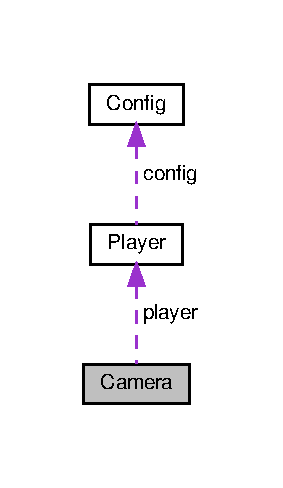
\includegraphics[width=136pt]{struct_camera__coll__graph}
\end{center}
\end{figure}
\subsection*{Открытые атрибуты}
\begin{DoxyCompactItemize}
\item 
string \hyperlink{struct_camera_a2adbd6da5cc41fb114c72b8616c00faf}{name}
\item 
string \hyperlink{struct_camera_a36dcf32b67cd3d0dcb45ab59fcc02cdb}{full\+Name}
\item 
string \hyperlink{struct_camera_a5d50a2e299b2cccd65b57982c678c8c4}{uri}
\item 
\hyperlink{class_player}{Player} $\ast$ \hyperlink{struct_camera_a9b1f95d3238bada633cf31b6e40c2d71}{player}
\item 
Gtk\+Widget $\ast$ \hyperlink{struct_camera_af463d4b36a2af1143d92b48cd5a8fa77}{button}
\item 
Gtk\+Widget $\ast$ \hyperlink{struct_camera_a6edbf520f8292d21ac6cccc61d45c41b}{drawing\+Area}
\item 
Gtk\+Widget $\ast$ \hyperlink{struct_camera_af6f95a716318992fa911c03349ec44f6}{rec\+Image}
\item 
bool \hyperlink{struct_camera_ab381a0e30d838132bea08b14686ea2f5}{record} = false
\end{DoxyCompactItemize}


\subsection{Данные класса}
\mbox{\Hypertarget{struct_camera_af463d4b36a2af1143d92b48cd5a8fa77}\label{struct_camera_af463d4b36a2af1143d92b48cd5a8fa77}} 
\index{Camera@{Camera}!button@{button}}
\index{button@{button}!Camera@{Camera}}
\subsubsection{\texorpdfstring{button}{button}}
{\footnotesize\ttfamily Gtk\+Widget $\ast$ Camera\+::button}

\mbox{\Hypertarget{struct_camera_a6edbf520f8292d21ac6cccc61d45c41b}\label{struct_camera_a6edbf520f8292d21ac6cccc61d45c41b}} 
\index{Camera@{Camera}!drawing\+Area@{drawing\+Area}}
\index{drawing\+Area@{drawing\+Area}!Camera@{Camera}}
\subsubsection{\texorpdfstring{drawing\+Area}{drawingArea}}
{\footnotesize\ttfamily Gtk\+Widget$\ast$ Camera\+::drawing\+Area}

\mbox{\Hypertarget{struct_camera_a36dcf32b67cd3d0dcb45ab59fcc02cdb}\label{struct_camera_a36dcf32b67cd3d0dcb45ab59fcc02cdb}} 
\index{Camera@{Camera}!full\+Name@{full\+Name}}
\index{full\+Name@{full\+Name}!Camera@{Camera}}
\subsubsection{\texorpdfstring{full\+Name}{fullName}}
{\footnotesize\ttfamily string Camera\+::full\+Name}

\mbox{\Hypertarget{struct_camera_a2adbd6da5cc41fb114c72b8616c00faf}\label{struct_camera_a2adbd6da5cc41fb114c72b8616c00faf}} 
\index{Camera@{Camera}!name@{name}}
\index{name@{name}!Camera@{Camera}}
\subsubsection{\texorpdfstring{name}{name}}
{\footnotesize\ttfamily string Camera\+::name}

\mbox{\Hypertarget{struct_camera_a9b1f95d3238bada633cf31b6e40c2d71}\label{struct_camera_a9b1f95d3238bada633cf31b6e40c2d71}} 
\index{Camera@{Camera}!player@{player}}
\index{player@{player}!Camera@{Camera}}
\subsubsection{\texorpdfstring{player}{player}}
{\footnotesize\ttfamily \hyperlink{class_player}{Player}$\ast$ Camera\+::player}

\mbox{\Hypertarget{struct_camera_af6f95a716318992fa911c03349ec44f6}\label{struct_camera_af6f95a716318992fa911c03349ec44f6}} 
\index{Camera@{Camera}!rec\+Image@{rec\+Image}}
\index{rec\+Image@{rec\+Image}!Camera@{Camera}}
\subsubsection{\texorpdfstring{rec\+Image}{recImage}}
{\footnotesize\ttfamily Gtk\+Widget$\ast$ Camera\+::rec\+Image}

\mbox{\Hypertarget{struct_camera_ab381a0e30d838132bea08b14686ea2f5}\label{struct_camera_ab381a0e30d838132bea08b14686ea2f5}} 
\index{Camera@{Camera}!record@{record}}
\index{record@{record}!Camera@{Camera}}
\subsubsection{\texorpdfstring{record}{record}}
{\footnotesize\ttfamily bool Camera\+::record = false}

\mbox{\Hypertarget{struct_camera_a5d50a2e299b2cccd65b57982c678c8c4}\label{struct_camera_a5d50a2e299b2cccd65b57982c678c8c4}} 
\index{Camera@{Camera}!uri@{uri}}
\index{uri@{uri}!Camera@{Camera}}
\subsubsection{\texorpdfstring{uri}{uri}}
{\footnotesize\ttfamily string Camera\+::uri}



Объявления и описания членов структуры находятся в файле\+:\begin{DoxyCompactItemize}
\item 
/home/jetson/controlroom/\+Studio/\+Operator/\+Grid/include/\hyperlink{_operator_2_grid_2include_2room_8h}{room.\+h}\end{DoxyCompactItemize}

\hypertarget{class_config}{}\section{Класс Config}
\label{class_config}\index{Config@{Config}}


The \hyperlink{class_config}{Config} class.  




{\ttfamily \#include $<$config.\+h$>$}

\subsection*{Открытые члены}
\begin{DoxyCompactItemize}
\item 
void \hyperlink{class_config_a06542bc14d3414c075a9cbb04f1e9a37}{set\+File} (string config\+Path)
\item 
string \hyperlink{class_config_ae20fcfa28d82f1d2d1a4387a00a9f8b2}{get\+Param} (string name)
\item 
int \hyperlink{class_config_a37b55073aa9e1a0e5a06323df5686c13}{get\+Param\+Int} (string name)
\item 
vector$<$ \hyperlink{class_room}{Room} $\ast$ $>$ $\ast$ \hyperlink{class_config_a644ff01239e20fabb038a2b2eddf1a26}{get\+Rooms} ()
\item 
void \hyperlink{class_config_a06542bc14d3414c075a9cbb04f1e9a37}{set\+File} (string config\+Path)
\item 
string \hyperlink{class_config_ae20fcfa28d82f1d2d1a4387a00a9f8b2}{get\+Param} (string name)
\item 
int \hyperlink{class_config_a37b55073aa9e1a0e5a06323df5686c13}{get\+Param\+Int} (string name)
\item 
vector$<$ \hyperlink{class_room}{Room} $\ast$ $>$ $\ast$ \hyperlink{class_config_ab10c3b7d3a76fcfa411ecba1dddc9716}{get\+Rooms} ()
\end{DoxyCompactItemize}
\subsection*{Открытые статические члены}
\begin{DoxyCompactItemize}
\item 
static \hyperlink{class_config}{Config} \& \hyperlink{class_config_a5154d96acc76c1fae8c564f3705fe197}{get} ()
\item 
static \hyperlink{class_config}{Config} \& \hyperlink{class_config_a5154d96acc76c1fae8c564f3705fe197}{get} ()
\end{DoxyCompactItemize}
\subsection*{Закрытые члены}
\begin{DoxyCompactItemize}
\item 
\hyperlink{class_config_abd0c571c116924871e30444b192b792a}{Config} ()
\item 
\hyperlink{class_config_add59e40b81cf0ffb43571bc201781dc0}{Config} (const \hyperlink{class_config}{Config} \&)
\item 
\hyperlink{class_config}{Config} \& \hyperlink{class_config_a301e8f32b1fad83bcab780bfa3fec1e9}{operator=} (const \hyperlink{class_config}{Config} \&)
\item 
void \hyperlink{class_config_a8a710b2b2b1e6280195389e9f84d0fba}{get\+G\+Suite\+Rooms} ()
\item 
void \hyperlink{class_config_af15e32047889f0d0e304cf4f5f218711}{get\+Custom\+Rooms} ()
\item 
string \hyperlink{class_config_a45dfcb0ab6def40b1ee15a0521a717ac}{make\+G\+Suite\+Request} ()
\item 
vector$<$ \hyperlink{class_room}{Room} $\ast$ $>$ \hyperlink{class_config_a585a61660c48877296ed9409c83b01c5}{read\+Rooms\+From\+File} (string file\+Name)
\item 
\hyperlink{class_config_abd0c571c116924871e30444b192b792a}{Config} ()
\item 
\hyperlink{class_config_add59e40b81cf0ffb43571bc201781dc0}{Config} (const \hyperlink{class_config}{Config} \&)
\item 
\hyperlink{class_config}{Config} \& \hyperlink{class_config_a301e8f32b1fad83bcab780bfa3fec1e9}{operator=} (const \hyperlink{class_config}{Config} \&)
\item 
void \hyperlink{class_config_a8a710b2b2b1e6280195389e9f84d0fba}{get\+G\+Suite\+Rooms} ()
\item 
void \hyperlink{class_config_af15e32047889f0d0e304cf4f5f218711}{get\+Custom\+Rooms} ()
\item 
string \hyperlink{class_config_a45dfcb0ab6def40b1ee15a0521a717ac}{make\+G\+Suite\+Request} ()
\item 
vector$<$ \hyperlink{class_room}{Room} $\ast$ $>$ \hyperlink{class_config_a8da1c4e1553854e6f248867f168de9ad}{read\+Rooms\+From\+File} (string file\+Name)
\end{DoxyCompactItemize}
\subsection*{Закрытые данные}
\begin{DoxyCompactItemize}
\item 
map$<$ string, string $>$ \hyperlink{class_config_a0b04d0c5fab98d257b2cf28cab895a3c}{configuration}
\item 
vector$<$ \hyperlink{class_room}{Room} $\ast$ $>$ \hyperlink{class_config_a13e9d9cfc3a9de64415d2674c6ecaf5c}{rooms}
\end{DoxyCompactItemize}


\subsection{Подробное описание}
The \hyperlink{class_config}{Config} class. 

Класс для хранения конфигурации

Данный класс выполнен по шаблону singleton. Читает конфигурацию из файла и хранит параметры в словаре (std\+::map). Вызывает from\+\_\+gsuite.\+py для получения данных о камерах из G\+Sutie. Читает файл gsuite\+\_\+rooms.\+json и создает объекты \hyperlink{class_room}{Room} для каждой комнаты, которые затем хранит в массиве (std\+::vector)

\subsection*{Форматирование файла конфигурации }

Файл должен содержать параметры из таблицы ниже, отформатированные в виде \#Комментарий Параметр = значение

\subsubsection*{Допустивые параметры }

\tabulinesep=1mm
\begin{longtabu} spread 0pt [c]{*{3}{|X[-1]}|}
\hline
\rowcolor{\tableheadbgcolor}\textbf{ Наименование }&\textbf{ Значение }&\textbf{ Описание  }\\\cline{1-3}
\endfirsthead
\hline
\endfoot
\hline
\rowcolor{\tableheadbgcolor}\textbf{ Наименование }&\textbf{ Значение }&\textbf{ Описание  }\\\cline{1-3}
\endhead
screens &1 или 2 &Количество используемых экранов \\\cline{1-3}
save\+To\+Folder &/путь &Путь к каталогу, в который будут сохраняться видеофайлы, начиная от корневого каталога системы (/) \\\cline{1-3}
window\+Width &Число (в пикселях) &Ширина и высота окон программы. Используется в случае, если параметр screens=1 \\\cline{1-3}
window\+Height &$^\wedge$ &$^\wedge$ \\\cline{1-3}
video\+Time\+Limit &Число(в минутах) &Ограничение на длительность видео в одном файле. \\\cline{1-3}
\end{longtabu}
\subsection*{Использование класса\+: }

\hyperlink{class_config}{Config} $\ast$config = \&\hyperlink{class_config_a5154d96acc76c1fae8c564f3705fe197}{Config\+::get()}; config-\/$>$set\+File(\char`\"{}recorder.\+conf\char`\"{}); config-\/$>$\hyperlink{class_config_a644ff01239e20fabb038a2b2eddf1a26}{get\+Rooms()} 

\subsection{Конструктор(ы)}
\mbox{\Hypertarget{class_config_abd0c571c116924871e30444b192b792a}\label{class_config_abd0c571c116924871e30444b192b792a}} 
\index{Config@{Config}!Config@{Config}}
\index{Config@{Config}!Config@{Config}}
\subsubsection{\texorpdfstring{Config()}{Config()}\hspace{0.1cm}{\footnotesize\ttfamily [1/4]}}
{\footnotesize\ttfamily Config\+::\+Config (\begin{DoxyParamCaption}{ }\end{DoxyParamCaption})\hspace{0.3cm}{\ttfamily [private]}}

Граф вызовов\+:\nopagebreak
\begin{figure}[H]
\begin{center}
\leavevmode
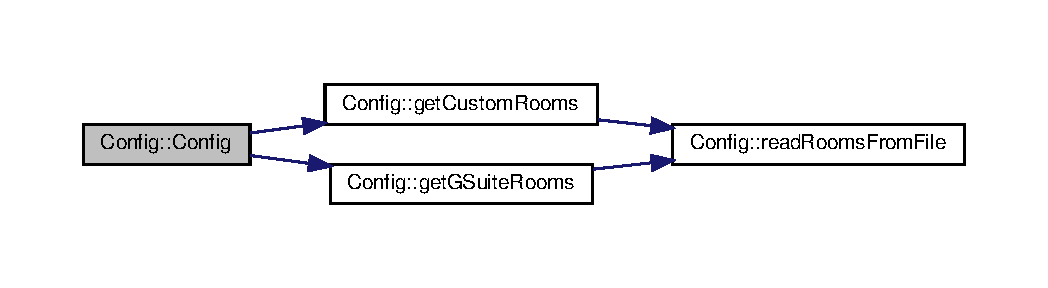
\includegraphics[width=350pt]{class_config_abd0c571c116924871e30444b192b792a_cgraph}
\end{center}
\end{figure}
\mbox{\Hypertarget{class_config_add59e40b81cf0ffb43571bc201781dc0}\label{class_config_add59e40b81cf0ffb43571bc201781dc0}} 
\index{Config@{Config}!Config@{Config}}
\index{Config@{Config}!Config@{Config}}
\subsubsection{\texorpdfstring{Config()}{Config()}\hspace{0.1cm}{\footnotesize\ttfamily [2/4]}}
{\footnotesize\ttfamily Config\+::\+Config (\begin{DoxyParamCaption}\item[{const \hyperlink{class_config}{Config} \&}]{ }\end{DoxyParamCaption})\hspace{0.3cm}{\ttfamily [private]}}

\mbox{\Hypertarget{class_config_abd0c571c116924871e30444b192b792a}\label{class_config_abd0c571c116924871e30444b192b792a}} 
\index{Config@{Config}!Config@{Config}}
\index{Config@{Config}!Config@{Config}}
\subsubsection{\texorpdfstring{Config()}{Config()}\hspace{0.1cm}{\footnotesize\ttfamily [3/4]}}
{\footnotesize\ttfamily Config\+::\+Config (\begin{DoxyParamCaption}{ }\end{DoxyParamCaption})\hspace{0.3cm}{\ttfamily [private]}}

\mbox{\Hypertarget{class_config_add59e40b81cf0ffb43571bc201781dc0}\label{class_config_add59e40b81cf0ffb43571bc201781dc0}} 
\index{Config@{Config}!Config@{Config}}
\index{Config@{Config}!Config@{Config}}
\subsubsection{\texorpdfstring{Config()}{Config()}\hspace{0.1cm}{\footnotesize\ttfamily [4/4]}}
{\footnotesize\ttfamily Config\+::\+Config (\begin{DoxyParamCaption}\item[{const \hyperlink{class_config}{Config} \&}]{ }\end{DoxyParamCaption})\hspace{0.3cm}{\ttfamily [private]}}



\subsection{Методы}
\mbox{\Hypertarget{class_config_a5154d96acc76c1fae8c564f3705fe197}\label{class_config_a5154d96acc76c1fae8c564f3705fe197}} 
\index{Config@{Config}!get@{get}}
\index{get@{get}!Config@{Config}}
\subsubsection{\texorpdfstring{get()}{get()}\hspace{0.1cm}{\footnotesize\ttfamily [1/2]}}
{\footnotesize\ttfamily static \hyperlink{class_config}{Config}\& Config\+::get (\begin{DoxyParamCaption}{ }\end{DoxyParamCaption})\hspace{0.3cm}{\ttfamily [inline]}, {\ttfamily [static]}}

\mbox{\Hypertarget{class_config_a5154d96acc76c1fae8c564f3705fe197}\label{class_config_a5154d96acc76c1fae8c564f3705fe197}} 
\index{Config@{Config}!get@{get}}
\index{get@{get}!Config@{Config}}
\subsubsection{\texorpdfstring{get()}{get()}\hspace{0.1cm}{\footnotesize\ttfamily [2/2]}}
{\footnotesize\ttfamily static \hyperlink{class_config}{Config}\& Config\+::get (\begin{DoxyParamCaption}{ }\end{DoxyParamCaption})\hspace{0.3cm}{\ttfamily [inline]}, {\ttfamily [static]}}

\mbox{\Hypertarget{class_config_af15e32047889f0d0e304cf4f5f218711}\label{class_config_af15e32047889f0d0e304cf4f5f218711}} 
\index{Config@{Config}!get\+Custom\+Rooms@{get\+Custom\+Rooms}}
\index{get\+Custom\+Rooms@{get\+Custom\+Rooms}!Config@{Config}}
\subsubsection{\texorpdfstring{get\+Custom\+Rooms()}{getCustomRooms()}\hspace{0.1cm}{\footnotesize\ttfamily [1/2]}}
{\footnotesize\ttfamily void Config\+::get\+Custom\+Rooms (\begin{DoxyParamCaption}{ }\end{DoxyParamCaption})\hspace{0.3cm}{\ttfamily [private]}}

Граф вызовов\+:\nopagebreak
\begin{figure}[H]
\begin{center}
\leavevmode
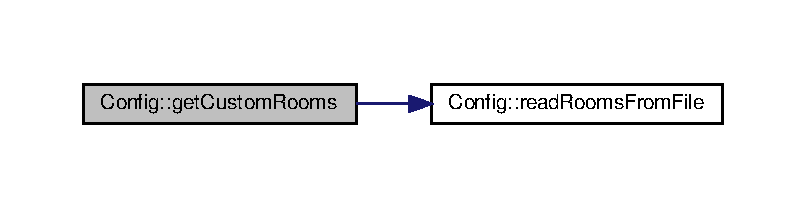
\includegraphics[width=350pt]{class_config_af15e32047889f0d0e304cf4f5f218711_cgraph}
\end{center}
\end{figure}
\mbox{\Hypertarget{class_config_af15e32047889f0d0e304cf4f5f218711}\label{class_config_af15e32047889f0d0e304cf4f5f218711}} 
\index{Config@{Config}!get\+Custom\+Rooms@{get\+Custom\+Rooms}}
\index{get\+Custom\+Rooms@{get\+Custom\+Rooms}!Config@{Config}}
\subsubsection{\texorpdfstring{get\+Custom\+Rooms()}{getCustomRooms()}\hspace{0.1cm}{\footnotesize\ttfamily [2/2]}}
{\footnotesize\ttfamily void Config\+::get\+Custom\+Rooms (\begin{DoxyParamCaption}{ }\end{DoxyParamCaption})\hspace{0.3cm}{\ttfamily [private]}}

\mbox{\Hypertarget{class_config_a8a710b2b2b1e6280195389e9f84d0fba}\label{class_config_a8a710b2b2b1e6280195389e9f84d0fba}} 
\index{Config@{Config}!get\+G\+Suite\+Rooms@{get\+G\+Suite\+Rooms}}
\index{get\+G\+Suite\+Rooms@{get\+G\+Suite\+Rooms}!Config@{Config}}
\subsubsection{\texorpdfstring{get\+G\+Suite\+Rooms()}{getGSuiteRooms()}\hspace{0.1cm}{\footnotesize\ttfamily [1/2]}}
{\footnotesize\ttfamily void Config\+::get\+G\+Suite\+Rooms (\begin{DoxyParamCaption}{ }\end{DoxyParamCaption})\hspace{0.3cm}{\ttfamily [private]}}

Граф вызовов\+:\nopagebreak
\begin{figure}[H]
\begin{center}
\leavevmode
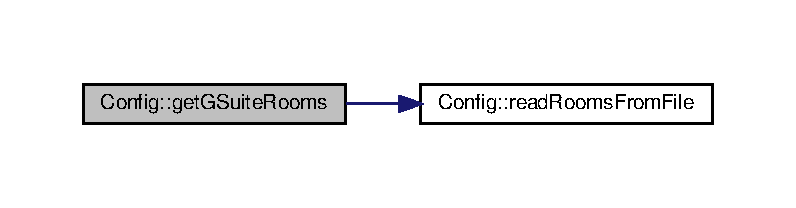
\includegraphics[width=350pt]{class_config_a8a710b2b2b1e6280195389e9f84d0fba_cgraph}
\end{center}
\end{figure}
\mbox{\Hypertarget{class_config_a8a710b2b2b1e6280195389e9f84d0fba}\label{class_config_a8a710b2b2b1e6280195389e9f84d0fba}} 
\index{Config@{Config}!get\+G\+Suite\+Rooms@{get\+G\+Suite\+Rooms}}
\index{get\+G\+Suite\+Rooms@{get\+G\+Suite\+Rooms}!Config@{Config}}
\subsubsection{\texorpdfstring{get\+G\+Suite\+Rooms()}{getGSuiteRooms()}\hspace{0.1cm}{\footnotesize\ttfamily [2/2]}}
{\footnotesize\ttfamily void Config\+::get\+G\+Suite\+Rooms (\begin{DoxyParamCaption}{ }\end{DoxyParamCaption})\hspace{0.3cm}{\ttfamily [private]}}

\mbox{\Hypertarget{class_config_ae20fcfa28d82f1d2d1a4387a00a9f8b2}\label{class_config_ae20fcfa28d82f1d2d1a4387a00a9f8b2}} 
\index{Config@{Config}!get\+Param@{get\+Param}}
\index{get\+Param@{get\+Param}!Config@{Config}}
\subsubsection{\texorpdfstring{get\+Param()}{getParam()}\hspace{0.1cm}{\footnotesize\ttfamily [1/2]}}
{\footnotesize\ttfamily string Config\+::get\+Param (\begin{DoxyParamCaption}\item[{string}]{name }\end{DoxyParamCaption})}

\mbox{\Hypertarget{class_config_ae20fcfa28d82f1d2d1a4387a00a9f8b2}\label{class_config_ae20fcfa28d82f1d2d1a4387a00a9f8b2}} 
\index{Config@{Config}!get\+Param@{get\+Param}}
\index{get\+Param@{get\+Param}!Config@{Config}}
\subsubsection{\texorpdfstring{get\+Param()}{getParam()}\hspace{0.1cm}{\footnotesize\ttfamily [2/2]}}
{\footnotesize\ttfamily string Config\+::get\+Param (\begin{DoxyParamCaption}\item[{string}]{name }\end{DoxyParamCaption})}

\mbox{\Hypertarget{class_config_a37b55073aa9e1a0e5a06323df5686c13}\label{class_config_a37b55073aa9e1a0e5a06323df5686c13}} 
\index{Config@{Config}!get\+Param\+Int@{get\+Param\+Int}}
\index{get\+Param\+Int@{get\+Param\+Int}!Config@{Config}}
\subsubsection{\texorpdfstring{get\+Param\+Int()}{getParamInt()}\hspace{0.1cm}{\footnotesize\ttfamily [1/2]}}
{\footnotesize\ttfamily int Config\+::get\+Param\+Int (\begin{DoxyParamCaption}\item[{string}]{name }\end{DoxyParamCaption})}

\mbox{\Hypertarget{class_config_a37b55073aa9e1a0e5a06323df5686c13}\label{class_config_a37b55073aa9e1a0e5a06323df5686c13}} 
\index{Config@{Config}!get\+Param\+Int@{get\+Param\+Int}}
\index{get\+Param\+Int@{get\+Param\+Int}!Config@{Config}}
\subsubsection{\texorpdfstring{get\+Param\+Int()}{getParamInt()}\hspace{0.1cm}{\footnotesize\ttfamily [2/2]}}
{\footnotesize\ttfamily int Config\+::get\+Param\+Int (\begin{DoxyParamCaption}\item[{string}]{name }\end{DoxyParamCaption})}

\mbox{\Hypertarget{class_config_a644ff01239e20fabb038a2b2eddf1a26}\label{class_config_a644ff01239e20fabb038a2b2eddf1a26}} 
\index{Config@{Config}!get\+Rooms@{get\+Rooms}}
\index{get\+Rooms@{get\+Rooms}!Config@{Config}}
\subsubsection{\texorpdfstring{get\+Rooms()}{getRooms()}\hspace{0.1cm}{\footnotesize\ttfamily [1/2]}}
{\footnotesize\ttfamily vector$<$ \hyperlink{class_room}{Room} $\ast$ $>$ $\ast$ Config\+::get\+Rooms (\begin{DoxyParamCaption}{ }\end{DoxyParamCaption})}

\mbox{\Hypertarget{class_config_ab10c3b7d3a76fcfa411ecba1dddc9716}\label{class_config_ab10c3b7d3a76fcfa411ecba1dddc9716}} 
\index{Config@{Config}!get\+Rooms@{get\+Rooms}}
\index{get\+Rooms@{get\+Rooms}!Config@{Config}}
\subsubsection{\texorpdfstring{get\+Rooms()}{getRooms()}\hspace{0.1cm}{\footnotesize\ttfamily [2/2]}}
{\footnotesize\ttfamily vector$<$\hyperlink{class_room}{Room}$\ast$$>$$\ast$ Config\+::get\+Rooms (\begin{DoxyParamCaption}{ }\end{DoxyParamCaption})}

\mbox{\Hypertarget{class_config_a45dfcb0ab6def40b1ee15a0521a717ac}\label{class_config_a45dfcb0ab6def40b1ee15a0521a717ac}} 
\index{Config@{Config}!make\+G\+Suite\+Request@{make\+G\+Suite\+Request}}
\index{make\+G\+Suite\+Request@{make\+G\+Suite\+Request}!Config@{Config}}
\subsubsection{\texorpdfstring{make\+G\+Suite\+Request()}{makeGSuiteRequest()}\hspace{0.1cm}{\footnotesize\ttfamily [1/2]}}
{\footnotesize\ttfamily string Config\+::make\+G\+Suite\+Request (\begin{DoxyParamCaption}{ }\end{DoxyParamCaption})\hspace{0.3cm}{\ttfamily [private]}}

\mbox{\Hypertarget{class_config_a45dfcb0ab6def40b1ee15a0521a717ac}\label{class_config_a45dfcb0ab6def40b1ee15a0521a717ac}} 
\index{Config@{Config}!make\+G\+Suite\+Request@{make\+G\+Suite\+Request}}
\index{make\+G\+Suite\+Request@{make\+G\+Suite\+Request}!Config@{Config}}
\subsubsection{\texorpdfstring{make\+G\+Suite\+Request()}{makeGSuiteRequest()}\hspace{0.1cm}{\footnotesize\ttfamily [2/2]}}
{\footnotesize\ttfamily string Config\+::make\+G\+Suite\+Request (\begin{DoxyParamCaption}{ }\end{DoxyParamCaption})\hspace{0.3cm}{\ttfamily [private]}}

\mbox{\Hypertarget{class_config_a301e8f32b1fad83bcab780bfa3fec1e9}\label{class_config_a301e8f32b1fad83bcab780bfa3fec1e9}} 
\index{Config@{Config}!operator=@{operator=}}
\index{operator=@{operator=}!Config@{Config}}
\subsubsection{\texorpdfstring{operator=()}{operator=()}\hspace{0.1cm}{\footnotesize\ttfamily [1/2]}}
{\footnotesize\ttfamily \hyperlink{class_config}{Config}\& Config\+::operator= (\begin{DoxyParamCaption}\item[{const \hyperlink{class_config}{Config} \&}]{ }\end{DoxyParamCaption})\hspace{0.3cm}{\ttfamily [private]}}

\mbox{\Hypertarget{class_config_a301e8f32b1fad83bcab780bfa3fec1e9}\label{class_config_a301e8f32b1fad83bcab780bfa3fec1e9}} 
\index{Config@{Config}!operator=@{operator=}}
\index{operator=@{operator=}!Config@{Config}}
\subsubsection{\texorpdfstring{operator=()}{operator=()}\hspace{0.1cm}{\footnotesize\ttfamily [2/2]}}
{\footnotesize\ttfamily \hyperlink{class_config}{Config}\& Config\+::operator= (\begin{DoxyParamCaption}\item[{const \hyperlink{class_config}{Config} \&}]{ }\end{DoxyParamCaption})\hspace{0.3cm}{\ttfamily [private]}}

\mbox{\Hypertarget{class_config_a585a61660c48877296ed9409c83b01c5}\label{class_config_a585a61660c48877296ed9409c83b01c5}} 
\index{Config@{Config}!read\+Rooms\+From\+File@{read\+Rooms\+From\+File}}
\index{read\+Rooms\+From\+File@{read\+Rooms\+From\+File}!Config@{Config}}
\subsubsection{\texorpdfstring{read\+Rooms\+From\+File()}{readRoomsFromFile()}\hspace{0.1cm}{\footnotesize\ttfamily [1/2]}}
{\footnotesize\ttfamily vector$<$ \hyperlink{class_room}{Room} $\ast$ $>$ Config\+::read\+Rooms\+From\+File (\begin{DoxyParamCaption}\item[{string}]{file\+Name }\end{DoxyParamCaption})\hspace{0.3cm}{\ttfamily [private]}}

\mbox{\Hypertarget{class_config_a8da1c4e1553854e6f248867f168de9ad}\label{class_config_a8da1c4e1553854e6f248867f168de9ad}} 
\index{Config@{Config}!read\+Rooms\+From\+File@{read\+Rooms\+From\+File}}
\index{read\+Rooms\+From\+File@{read\+Rooms\+From\+File}!Config@{Config}}
\subsubsection{\texorpdfstring{read\+Rooms\+From\+File()}{readRoomsFromFile()}\hspace{0.1cm}{\footnotesize\ttfamily [2/2]}}
{\footnotesize\ttfamily vector$<$\hyperlink{class_room}{Room}$\ast$$>$ Config\+::read\+Rooms\+From\+File (\begin{DoxyParamCaption}\item[{string}]{file\+Name }\end{DoxyParamCaption})\hspace{0.3cm}{\ttfamily [private]}}

\mbox{\Hypertarget{class_config_a06542bc14d3414c075a9cbb04f1e9a37}\label{class_config_a06542bc14d3414c075a9cbb04f1e9a37}} 
\index{Config@{Config}!set\+File@{set\+File}}
\index{set\+File@{set\+File}!Config@{Config}}
\subsubsection{\texorpdfstring{set\+File()}{setFile()}\hspace{0.1cm}{\footnotesize\ttfamily [1/2]}}
{\footnotesize\ttfamily void Config\+::set\+File (\begin{DoxyParamCaption}\item[{string}]{config\+Path }\end{DoxyParamCaption})}

\mbox{\Hypertarget{class_config_a06542bc14d3414c075a9cbb04f1e9a37}\label{class_config_a06542bc14d3414c075a9cbb04f1e9a37}} 
\index{Config@{Config}!set\+File@{set\+File}}
\index{set\+File@{set\+File}!Config@{Config}}
\subsubsection{\texorpdfstring{set\+File()}{setFile()}\hspace{0.1cm}{\footnotesize\ttfamily [2/2]}}
{\footnotesize\ttfamily void Config\+::set\+File (\begin{DoxyParamCaption}\item[{string}]{config\+Path }\end{DoxyParamCaption})}



\subsection{Данные класса}
\mbox{\Hypertarget{class_config_a0b04d0c5fab98d257b2cf28cab895a3c}\label{class_config_a0b04d0c5fab98d257b2cf28cab895a3c}} 
\index{Config@{Config}!configuration@{configuration}}
\index{configuration@{configuration}!Config@{Config}}
\subsubsection{\texorpdfstring{configuration}{configuration}}
{\footnotesize\ttfamily map$<$ string, string $>$ Config\+::configuration\hspace{0.3cm}{\ttfamily [private]}}

\mbox{\Hypertarget{class_config_a13e9d9cfc3a9de64415d2674c6ecaf5c}\label{class_config_a13e9d9cfc3a9de64415d2674c6ecaf5c}} 
\index{Config@{Config}!rooms@{rooms}}
\index{rooms@{rooms}!Config@{Config}}
\subsubsection{\texorpdfstring{rooms}{rooms}}
{\footnotesize\ttfamily vector$<$ \hyperlink{class_room}{Room} $\ast$ $>$ Config\+::rooms\hspace{0.3cm}{\ttfamily [private]}}



Объявления и описания членов классов находятся в файлах\+:\begin{DoxyCompactItemize}
\item 
/home/jetson/controlroom/\+Studio/\+Operator/\+Grid/include/\hyperlink{_operator_2_grid_2include_2config_8h}{config.\+h}\item 
/home/jetson/controlroom/\+Studio/\+Operator/\+Grid/src/\hyperlink{_operator_2_grid_2src_2config_8cpp}{config.\+cpp}\end{DoxyCompactItemize}

\hypertarget{struct_u_i_1_1display__player__data}{}\section{Структура UI\+:\+:display\+\_\+player\+\_\+data}
\label{struct_u_i_1_1display__player__data}\index{U\+I\+::display\+\_\+player\+\_\+data@{U\+I\+::display\+\_\+player\+\_\+data}}


Граф связей класса UI\+:\+:display\+\_\+player\+\_\+data\+:\nopagebreak
\begin{figure}[H]
\begin{center}
\leavevmode
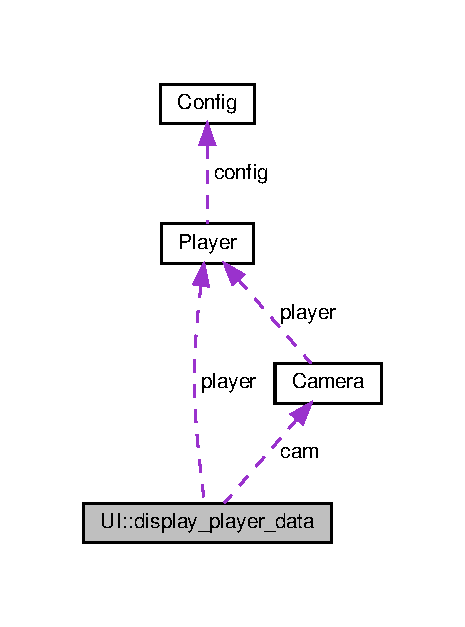
\includegraphics[width=223pt]{struct_u_i_1_1display__player__data__coll__graph}
\end{center}
\end{figure}
\subsection*{Открытые атрибуты}
\begin{DoxyCompactItemize}
\item 
\hyperlink{struct_camera}{Camera} \hyperlink{struct_u_i_1_1display__player__data_aaf6faafe9187df11c613189bb62cfe7d}{cam}
\item 
string $\ast$ \hyperlink{struct_u_i_1_1display__player__data_afc4f178e4761d152f91822cd5a070669}{playing\+Cam\+Name}
\item 
Gtk\+Widget $\ast$ \hyperlink{struct_u_i_1_1display__player__data_af5f6fe2e056926b9b804cdaeaaecc463}{player\+Label}
\item 
\hyperlink{class_player}{Player} $\ast$ \hyperlink{struct_u_i_1_1display__player__data_a05ff8238e08b44593287a350c98a80ba}{player}
\end{DoxyCompactItemize}


\subsection{Данные класса}
\mbox{\Hypertarget{struct_u_i_1_1display__player__data_aaf6faafe9187df11c613189bb62cfe7d}\label{struct_u_i_1_1display__player__data_aaf6faafe9187df11c613189bb62cfe7d}} 
\index{U\+I\+::display\+\_\+player\+\_\+data@{U\+I\+::display\+\_\+player\+\_\+data}!cam@{cam}}
\index{cam@{cam}!U\+I\+::display\+\_\+player\+\_\+data@{U\+I\+::display\+\_\+player\+\_\+data}}
\subsubsection{\texorpdfstring{cam}{cam}}
{\footnotesize\ttfamily \hyperlink{struct_camera}{Camera} U\+I\+::display\+\_\+player\+\_\+data\+::cam}

\mbox{\Hypertarget{struct_u_i_1_1display__player__data_a05ff8238e08b44593287a350c98a80ba}\label{struct_u_i_1_1display__player__data_a05ff8238e08b44593287a350c98a80ba}} 
\index{U\+I\+::display\+\_\+player\+\_\+data@{U\+I\+::display\+\_\+player\+\_\+data}!player@{player}}
\index{player@{player}!U\+I\+::display\+\_\+player\+\_\+data@{U\+I\+::display\+\_\+player\+\_\+data}}
\subsubsection{\texorpdfstring{player}{player}}
{\footnotesize\ttfamily \hyperlink{class_player}{Player}$\ast$ U\+I\+::display\+\_\+player\+\_\+data\+::player}

\mbox{\Hypertarget{struct_u_i_1_1display__player__data_af5f6fe2e056926b9b804cdaeaaecc463}\label{struct_u_i_1_1display__player__data_af5f6fe2e056926b9b804cdaeaaecc463}} 
\index{U\+I\+::display\+\_\+player\+\_\+data@{U\+I\+::display\+\_\+player\+\_\+data}!player\+Label@{player\+Label}}
\index{player\+Label@{player\+Label}!U\+I\+::display\+\_\+player\+\_\+data@{U\+I\+::display\+\_\+player\+\_\+data}}
\subsubsection{\texorpdfstring{player\+Label}{playerLabel}}
{\footnotesize\ttfamily Gtk\+Widget$\ast$ U\+I\+::display\+\_\+player\+\_\+data\+::player\+Label}

\mbox{\Hypertarget{struct_u_i_1_1display__player__data_afc4f178e4761d152f91822cd5a070669}\label{struct_u_i_1_1display__player__data_afc4f178e4761d152f91822cd5a070669}} 
\index{U\+I\+::display\+\_\+player\+\_\+data@{U\+I\+::display\+\_\+player\+\_\+data}!playing\+Cam\+Name@{playing\+Cam\+Name}}
\index{playing\+Cam\+Name@{playing\+Cam\+Name}!U\+I\+::display\+\_\+player\+\_\+data@{U\+I\+::display\+\_\+player\+\_\+data}}
\subsubsection{\texorpdfstring{playing\+Cam\+Name}{playingCamName}}
{\footnotesize\ttfamily string $\ast$ U\+I\+::display\+\_\+player\+\_\+data\+::playing\+Cam\+Name}



Объявления и описания членов структуры находятся в файле\+:\begin{DoxyCompactItemize}
\item 
/home/jetson/controlroom/\+Studio/\+Operator/\+Grid/include/\hyperlink{_operator_2_grid_2include_2ui_8h}{ui.\+h}\end{DoxyCompactItemize}

\hypertarget{struct_u_i_1_1gdrive__status__data}{}\section{Структура UI\+:\+:gdrive\+\_\+status\+\_\+data}
\label{struct_u_i_1_1gdrive__status__data}\index{U\+I\+::gdrive\+\_\+status\+\_\+data@{U\+I\+::gdrive\+\_\+status\+\_\+data}}


Граф связей класса UI\+:\+:gdrive\+\_\+status\+\_\+data\+:\nopagebreak
\begin{figure}[H]
\begin{center}
\leavevmode
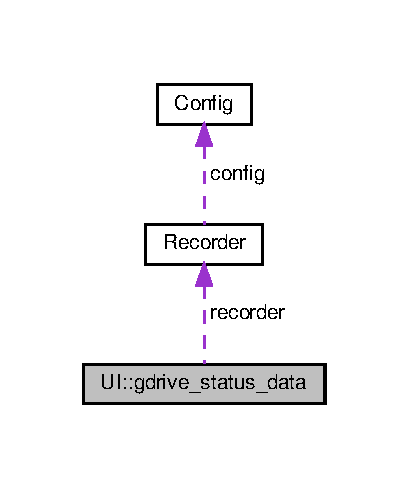
\includegraphics[width=196pt]{struct_u_i_1_1gdrive__status__data__coll__graph}
\end{center}
\end{figure}
\subsection*{Открытые атрибуты}
\begin{DoxyCompactItemize}
\item 
\hyperlink{class_recorder}{Recorder} $\ast$ \hyperlink{struct_u_i_1_1gdrive__status__data_a8634b4af863a719fe24b39b88ab103a9}{recorder}
\item 
Gtk\+Widget $\ast$ \hyperlink{struct_u_i_1_1gdrive__status__data_a7c780ddf23f96c083557c889efd85130}{G\+Drive\+Icon}
\end{DoxyCompactItemize}


\subsection{Данные класса}
\mbox{\Hypertarget{struct_u_i_1_1gdrive__status__data_a7c780ddf23f96c083557c889efd85130}\label{struct_u_i_1_1gdrive__status__data_a7c780ddf23f96c083557c889efd85130}} 
\index{U\+I\+::gdrive\+\_\+status\+\_\+data@{U\+I\+::gdrive\+\_\+status\+\_\+data}!G\+Drive\+Icon@{G\+Drive\+Icon}}
\index{G\+Drive\+Icon@{G\+Drive\+Icon}!U\+I\+::gdrive\+\_\+status\+\_\+data@{U\+I\+::gdrive\+\_\+status\+\_\+data}}
\subsubsection{\texorpdfstring{G\+Drive\+Icon}{GDriveIcon}}
{\footnotesize\ttfamily Gtk\+Widget$\ast$ U\+I\+::gdrive\+\_\+status\+\_\+data\+::\+G\+Drive\+Icon}

\mbox{\Hypertarget{struct_u_i_1_1gdrive__status__data_a8634b4af863a719fe24b39b88ab103a9}\label{struct_u_i_1_1gdrive__status__data_a8634b4af863a719fe24b39b88ab103a9}} 
\index{U\+I\+::gdrive\+\_\+status\+\_\+data@{U\+I\+::gdrive\+\_\+status\+\_\+data}!recorder@{recorder}}
\index{recorder@{recorder}!U\+I\+::gdrive\+\_\+status\+\_\+data@{U\+I\+::gdrive\+\_\+status\+\_\+data}}
\subsubsection{\texorpdfstring{recorder}{recorder}}
{\footnotesize\ttfamily \hyperlink{class_recorder}{Recorder}$\ast$ U\+I\+::gdrive\+\_\+status\+\_\+data\+::recorder}



Объявления и описания членов структуры находятся в файле\+:\begin{DoxyCompactItemize}
\item 
/home/jetson/controlroom/\+Studio/\+Recorder/include/\hyperlink{_recorder_2include_2ui_8h}{ui.\+h}\end{DoxyCompactItemize}

\hypertarget{classnetwork__monitor_1_1_grapher}{}\section{Класс network\+\_\+monitor.\+Grapher}
\label{classnetwork__monitor_1_1_grapher}\index{network\+\_\+monitor.\+Grapher@{network\+\_\+monitor.\+Grapher}}
\subsection*{Открытые члены}
\begin{DoxyCompactItemize}
\item 
def \hyperlink{classnetwork__monitor_1_1_grapher_a51113dd8de2a23b04c7d21e05443a254}{\+\_\+\+\_\+init\+\_\+\+\_\+} (self, \hyperlink{classnetwork__monitor_1_1_grapher_a3ebf5396c625164b8ef6477aeabfcd2d}{plot})
\item 
def \hyperlink{classnetwork__monitor_1_1_grapher_a6eb6ea6a4d6c3759f8182fdf07432cb5}{set\+Data} (self, cam, \hyperlink{classnetwork__monitor_1_1_grapher_aa4de1f707991945eff5ad4836ace2369}{data})
\item 
def \hyperlink{classnetwork__monitor_1_1_grapher_a424bf8aa9aead01ea95c2a52744dfb37}{change\+Cam} (self, cam)
\end{DoxyCompactItemize}
\subsection*{Открытые атрибуты}
\begin{DoxyCompactItemize}
\item 
\hyperlink{classnetwork__monitor_1_1_grapher_a3ebf5396c625164b8ef6477aeabfcd2d}{plot}
\item 
\hyperlink{classnetwork__monitor_1_1_grapher_ac014cfb815646074bf97e975af0ed774}{curve}
\item 
\hyperlink{classnetwork__monitor_1_1_grapher_a423a9b2f9d50d5fff7a12eaa81cbc4ad}{active\+Cam}
\item 
\hyperlink{classnetwork__monitor_1_1_grapher_aa4de1f707991945eff5ad4836ace2369}{data}
\end{DoxyCompactItemize}


\subsection{Подробное описание}
\begin{DoxyVerb}Draws a graph on PlotWidget\end{DoxyVerb}
 

\subsection{Конструктор(ы)}
\mbox{\Hypertarget{classnetwork__monitor_1_1_grapher_a51113dd8de2a23b04c7d21e05443a254}\label{classnetwork__monitor_1_1_grapher_a51113dd8de2a23b04c7d21e05443a254}} 
\index{network\+\_\+monitor\+::\+Grapher@{network\+\_\+monitor\+::\+Grapher}!\+\_\+\+\_\+init\+\_\+\+\_\+@{\+\_\+\+\_\+init\+\_\+\+\_\+}}
\index{\+\_\+\+\_\+init\+\_\+\+\_\+@{\+\_\+\+\_\+init\+\_\+\+\_\+}!network\+\_\+monitor\+::\+Grapher@{network\+\_\+monitor\+::\+Grapher}}
\subsubsection{\texorpdfstring{\+\_\+\+\_\+init\+\_\+\+\_\+()}{\_\_init\_\_()}}
{\footnotesize\ttfamily def network\+\_\+monitor.\+Grapher.\+\_\+\+\_\+init\+\_\+\+\_\+ (\begin{DoxyParamCaption}\item[{}]{self,  }\item[{}]{plot }\end{DoxyParamCaption})}



\subsection{Методы}
\mbox{\Hypertarget{classnetwork__monitor_1_1_grapher_a424bf8aa9aead01ea95c2a52744dfb37}\label{classnetwork__monitor_1_1_grapher_a424bf8aa9aead01ea95c2a52744dfb37}} 
\index{network\+\_\+monitor\+::\+Grapher@{network\+\_\+monitor\+::\+Grapher}!change\+Cam@{change\+Cam}}
\index{change\+Cam@{change\+Cam}!network\+\_\+monitor\+::\+Grapher@{network\+\_\+monitor\+::\+Grapher}}
\subsubsection{\texorpdfstring{change\+Cam()}{changeCam()}}
{\footnotesize\ttfamily def network\+\_\+monitor.\+Grapher.\+change\+Cam (\begin{DoxyParamCaption}\item[{}]{self,  }\item[{}]{cam }\end{DoxyParamCaption})}

\begin{DoxyVerb}Set name or ip of camera, which data should be drawn\end{DoxyVerb}
 \mbox{\Hypertarget{classnetwork__monitor_1_1_grapher_a6eb6ea6a4d6c3759f8182fdf07432cb5}\label{classnetwork__monitor_1_1_grapher_a6eb6ea6a4d6c3759f8182fdf07432cb5}} 
\index{network\+\_\+monitor\+::\+Grapher@{network\+\_\+monitor\+::\+Grapher}!set\+Data@{set\+Data}}
\index{set\+Data@{set\+Data}!network\+\_\+monitor\+::\+Grapher@{network\+\_\+monitor\+::\+Grapher}}
\subsubsection{\texorpdfstring{set\+Data()}{setData()}}
{\footnotesize\ttfamily def network\+\_\+monitor.\+Grapher.\+set\+Data (\begin{DoxyParamCaption}\item[{}]{self,  }\item[{}]{cam,  }\item[{}]{data }\end{DoxyParamCaption})}



\subsection{Данные класса}
\mbox{\Hypertarget{classnetwork__monitor_1_1_grapher_a423a9b2f9d50d5fff7a12eaa81cbc4ad}\label{classnetwork__monitor_1_1_grapher_a423a9b2f9d50d5fff7a12eaa81cbc4ad}} 
\index{network\+\_\+monitor\+::\+Grapher@{network\+\_\+monitor\+::\+Grapher}!active\+Cam@{active\+Cam}}
\index{active\+Cam@{active\+Cam}!network\+\_\+monitor\+::\+Grapher@{network\+\_\+monitor\+::\+Grapher}}
\subsubsection{\texorpdfstring{active\+Cam}{activeCam}}
{\footnotesize\ttfamily network\+\_\+monitor.\+Grapher.\+active\+Cam}

\mbox{\Hypertarget{classnetwork__monitor_1_1_grapher_ac014cfb815646074bf97e975af0ed774}\label{classnetwork__monitor_1_1_grapher_ac014cfb815646074bf97e975af0ed774}} 
\index{network\+\_\+monitor\+::\+Grapher@{network\+\_\+monitor\+::\+Grapher}!curve@{curve}}
\index{curve@{curve}!network\+\_\+monitor\+::\+Grapher@{network\+\_\+monitor\+::\+Grapher}}
\subsubsection{\texorpdfstring{curve}{curve}}
{\footnotesize\ttfamily network\+\_\+monitor.\+Grapher.\+curve}

\mbox{\Hypertarget{classnetwork__monitor_1_1_grapher_aa4de1f707991945eff5ad4836ace2369}\label{classnetwork__monitor_1_1_grapher_aa4de1f707991945eff5ad4836ace2369}} 
\index{network\+\_\+monitor\+::\+Grapher@{network\+\_\+monitor\+::\+Grapher}!data@{data}}
\index{data@{data}!network\+\_\+monitor\+::\+Grapher@{network\+\_\+monitor\+::\+Grapher}}
\subsubsection{\texorpdfstring{data}{data}}
{\footnotesize\ttfamily network\+\_\+monitor.\+Grapher.\+data}

\mbox{\Hypertarget{classnetwork__monitor_1_1_grapher_a3ebf5396c625164b8ef6477aeabfcd2d}\label{classnetwork__monitor_1_1_grapher_a3ebf5396c625164b8ef6477aeabfcd2d}} 
\index{network\+\_\+monitor\+::\+Grapher@{network\+\_\+monitor\+::\+Grapher}!plot@{plot}}
\index{plot@{plot}!network\+\_\+monitor\+::\+Grapher@{network\+\_\+monitor\+::\+Grapher}}
\subsubsection{\texorpdfstring{plot}{plot}}
{\footnotesize\ttfamily network\+\_\+monitor.\+Grapher.\+plot}



Объявления и описания членов класса находятся в файле\+:\begin{DoxyCompactItemize}
\item 
/home/jetson/controlroom/\+Studio/\+Network/src/\hyperlink{network__monitor_8py}{network\+\_\+monitor.\+py}\end{DoxyCompactItemize}

\hypertarget{struct_pad_data}{}\section{Структура Pad\+Data}
\label{struct_pad_data}\index{Pad\+Data@{Pad\+Data}}


{\ttfamily \#include $<$player.\+h$>$}

\subsection*{Открытые атрибуты}
\begin{DoxyCompactItemize}
\item 
Gst\+Element $\ast$ \hyperlink{struct_pad_data_a2dcc36381541106e5f4d2a8eba93c743}{src}
\item 
Gst\+Element $\ast$ \hyperlink{struct_pad_data_acd71290a8ca04825f41627151fd4caa3}{depay}
\end{DoxyCompactItemize}


\subsection{Данные класса}
\mbox{\Hypertarget{struct_pad_data_acd71290a8ca04825f41627151fd4caa3}\label{struct_pad_data_acd71290a8ca04825f41627151fd4caa3}} 
\index{Pad\+Data@{Pad\+Data}!depay@{depay}}
\index{depay@{depay}!Pad\+Data@{Pad\+Data}}
\subsubsection{\texorpdfstring{depay}{depay}}
{\footnotesize\ttfamily Gst\+Element $\ast$ Pad\+Data\+::depay}

\mbox{\Hypertarget{struct_pad_data_a2dcc36381541106e5f4d2a8eba93c743}\label{struct_pad_data_a2dcc36381541106e5f4d2a8eba93c743}} 
\index{Pad\+Data@{Pad\+Data}!src@{src}}
\index{src@{src}!Pad\+Data@{Pad\+Data}}
\subsubsection{\texorpdfstring{src}{src}}
{\footnotesize\ttfamily Gst\+Element $\ast$ Pad\+Data\+::src}



Объявления и описания членов структуры находятся в файле\+:\begin{DoxyCompactItemize}
\item 
/home/jetson/controlroom/\+Studio/\+Operator/\+Grid/include/\hyperlink{_operator_2_grid_2include_2player_8h}{player.\+h}\end{DoxyCompactItemize}

\hypertarget{classnetwork__monitor_1_1_pinger}{}\section{Класс network\+\_\+monitor.\+Pinger}
\label{classnetwork__monitor_1_1_pinger}\index{network\+\_\+monitor.\+Pinger@{network\+\_\+monitor.\+Pinger}}


Пингует камеры  




Граф наследования\+:network\+\_\+monitor.\+Pinger\+:\nopagebreak
\begin{figure}[H]
\begin{center}
\leavevmode
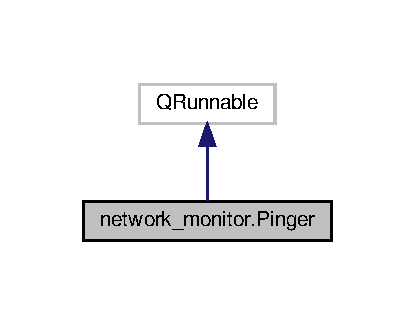
\includegraphics[width=199pt]{classnetwork__monitor_1_1_pinger__inherit__graph}
\end{center}
\end{figure}


Граф связей класса network\+\_\+monitor.\+Pinger\+:\nopagebreak
\begin{figure}[H]
\begin{center}
\leavevmode
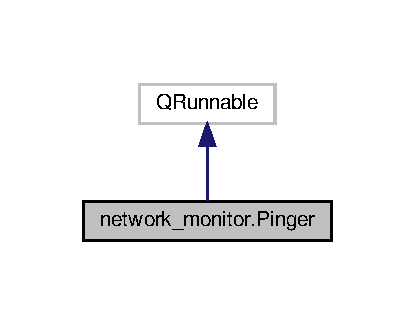
\includegraphics[width=199pt]{classnetwork__monitor_1_1_pinger__coll__graph}
\end{center}
\end{figure}
\subsection*{Открытые члены}
\begin{DoxyCompactItemize}
\item 
def \hyperlink{classnetwork__monitor_1_1_pinger_aa24b595bfd313e99ec0e0e9bd2f648d0}{\+\_\+\+\_\+init\+\_\+\+\_\+} (self, \hyperlink{classnetwork__monitor_1_1_pinger_a9e16cc56e9483b16869dccd9b87045d9}{cam\+List})
\item 
def \hyperlink{classnetwork__monitor_1_1_pinger_aa316109fda2807e15b9edaa947f4a724}{run} (self)
\end{DoxyCompactItemize}
\subsection*{Открытые атрибуты}
\begin{DoxyCompactItemize}
\item 
\hyperlink{classnetwork__monitor_1_1_pinger_a9e16cc56e9483b16869dccd9b87045d9}{cam\+List}
\end{DoxyCompactItemize}
\subsection*{Закрытые члены}
\begin{DoxyCompactItemize}
\item 
def \hyperlink{classnetwork__monitor_1_1_pinger_a8fa23184da9cbc4a3cafa6b08aee2cde}{\+\_\+run\+Cmd} (self, cmd, stderr=S\+T\+D\+O\+UT)
\end{DoxyCompactItemize}


\subsection{Подробное описание}
Пингует камеры 

\begin{DoxyVerb}Updates ping information \end{DoxyVerb}
 

\subsection{Конструктор(ы)}
\mbox{\Hypertarget{classnetwork__monitor_1_1_pinger_aa24b595bfd313e99ec0e0e9bd2f648d0}\label{classnetwork__monitor_1_1_pinger_aa24b595bfd313e99ec0e0e9bd2f648d0}} 
\index{network\+\_\+monitor\+::\+Pinger@{network\+\_\+monitor\+::\+Pinger}!\+\_\+\+\_\+init\+\_\+\+\_\+@{\+\_\+\+\_\+init\+\_\+\+\_\+}}
\index{\+\_\+\+\_\+init\+\_\+\+\_\+@{\+\_\+\+\_\+init\+\_\+\+\_\+}!network\+\_\+monitor\+::\+Pinger@{network\+\_\+monitor\+::\+Pinger}}
\subsubsection{\texorpdfstring{\+\_\+\+\_\+init\+\_\+\+\_\+()}{\_\_init\_\_()}}
{\footnotesize\ttfamily def network\+\_\+monitor.\+Pinger.\+\_\+\+\_\+init\+\_\+\+\_\+ (\begin{DoxyParamCaption}\item[{}]{self,  }\item[{}]{cam\+List }\end{DoxyParamCaption})}



\subsection{Методы}
\mbox{\Hypertarget{classnetwork__monitor_1_1_pinger_a8fa23184da9cbc4a3cafa6b08aee2cde}\label{classnetwork__monitor_1_1_pinger_a8fa23184da9cbc4a3cafa6b08aee2cde}} 
\index{network\+\_\+monitor\+::\+Pinger@{network\+\_\+monitor\+::\+Pinger}!\+\_\+run\+Cmd@{\+\_\+run\+Cmd}}
\index{\+\_\+run\+Cmd@{\+\_\+run\+Cmd}!network\+\_\+monitor\+::\+Pinger@{network\+\_\+monitor\+::\+Pinger}}
\subsubsection{\texorpdfstring{\+\_\+run\+Cmd()}{\_runCmd()}}
{\footnotesize\ttfamily def network\+\_\+monitor.\+Pinger.\+\_\+run\+Cmd (\begin{DoxyParamCaption}\item[{}]{self,  }\item[{}]{cmd,  }\item[{}]{stderr = {\ttfamily STDOUT} }\end{DoxyParamCaption})\hspace{0.3cm}{\ttfamily [private]}}

\begin{DoxyVerb}Run commend and get output \end{DoxyVerb}
 \mbox{\Hypertarget{classnetwork__monitor_1_1_pinger_aa316109fda2807e15b9edaa947f4a724}\label{classnetwork__monitor_1_1_pinger_aa316109fda2807e15b9edaa947f4a724}} 
\index{network\+\_\+monitor\+::\+Pinger@{network\+\_\+monitor\+::\+Pinger}!run@{run}}
\index{run@{run}!network\+\_\+monitor\+::\+Pinger@{network\+\_\+monitor\+::\+Pinger}}
\subsubsection{\texorpdfstring{run()}{run()}}
{\footnotesize\ttfamily def network\+\_\+monitor.\+Pinger.\+run (\begin{DoxyParamCaption}\item[{}]{self }\end{DoxyParamCaption})}

\begin{DoxyVerb}Function for QThreadPool to run in separate thread \end{DoxyVerb}
 Граф вызовов\+:\nopagebreak
\begin{figure}[H]
\begin{center}
\leavevmode
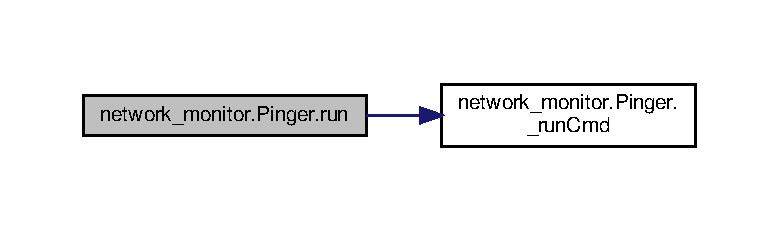
\includegraphics[width=350pt]{classnetwork__monitor_1_1_pinger_aa316109fda2807e15b9edaa947f4a724_cgraph}
\end{center}
\end{figure}


\subsection{Данные класса}
\mbox{\Hypertarget{classnetwork__monitor_1_1_pinger_a9e16cc56e9483b16869dccd9b87045d9}\label{classnetwork__monitor_1_1_pinger_a9e16cc56e9483b16869dccd9b87045d9}} 
\index{network\+\_\+monitor\+::\+Pinger@{network\+\_\+monitor\+::\+Pinger}!cam\+List@{cam\+List}}
\index{cam\+List@{cam\+List}!network\+\_\+monitor\+::\+Pinger@{network\+\_\+monitor\+::\+Pinger}}
\subsubsection{\texorpdfstring{cam\+List}{camList}}
{\footnotesize\ttfamily network\+\_\+monitor.\+Pinger.\+cam\+List}



Объявления и описания членов класса находятся в файле\+:\begin{DoxyCompactItemize}
\item 
/home/jetson/controlroom/\+Studio/\+Network/src/\hyperlink{network__monitor_8py}{network\+\_\+monitor.\+py}\end{DoxyCompactItemize}

\hypertarget{class_player}{}\section{Класс Player}
\label{class_player}\index{Player@{Player}}


The \hyperlink{class_player}{Player} class.  




{\ttfamily \#include $<$player.\+h$>$}



Граф связей класса Player\+:\nopagebreak
\begin{figure}[H]
\begin{center}
\leavevmode
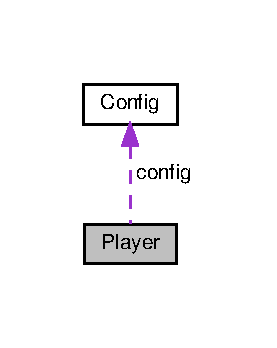
\includegraphics[width=133pt]{class_player__coll__graph}
\end{center}
\end{figure}
\subsection*{Открытые члены}
\begin{DoxyCompactItemize}
\item 
\hyperlink{class_player_a0e17f3ec3397aa056d2ee88a060a7d36}{Player} (Gtk\+Widget $\ast$\hyperlink{class_player_ae5ed3420e43869788a3e9bf4eb29e529}{video\+Window}, string \hyperlink{class_player_a4335f10f38749272bbdee425e8e30388}{platform}, string \hyperlink{class_player_a02eaaec54dce5238f76ef6b9f458c86d}{uri}, string \hyperlink{class_player_af5647b79bedfd422ca8758c90c6bbc45}{cam\+Name})
\item 
\hyperlink{class_player_a749d2c00e1fe0f5c2746f7505a58c062}{$\sim$\+Player} ()
\item 
void \hyperlink{class_player_a082180138fe92098aa9a1f51fd9ad40d}{play\+Stream} ()
\item 
void \hyperlink{class_player_aa8396672dd38d93e1000b7b0f55e9c24}{stop\+Stream} ()
\item 
bool \hyperlink{class_player_a370339dfdf9eb61905637283a72f9e22}{is\+Playing} ()
\item 
\hyperlink{class_player_a4b179b1c59f780f59e215fa5642acb99}{Player} (Gtk\+Widget $\ast$\hyperlink{class_player_ae5ed3420e43869788a3e9bf4eb29e529}{video\+Window}, \hyperlink{class_config}{Config} $\ast$\hyperlink{class_player_a53cd9b524dac60ecacd99f0812c71332}{config})
\item 
\hyperlink{class_player_a749d2c00e1fe0f5c2746f7505a58c062}{$\sim$\+Player} ()
\item 
void \hyperlink{class_player_a75c7257813c5f96bb2d8585dfc0c3025}{play\+Stream} (string \hyperlink{class_player_a02eaaec54dce5238f76ef6b9f458c86d}{uri})
\end{DoxyCompactItemize}
\subsection*{Открытые атрибуты}
\begin{DoxyCompactItemize}
\item 
Gst\+Element $\ast$ \hyperlink{class_player_aa8cd0e05525fd7cf5ee60b40b1388254}{pipeline}
\item 
Gst\+Element $\ast$ \hyperlink{class_player_ac3fb217cb2001134249fafcba07fe7e7}{src}
\item 
Gst\+Element $\ast$ \hyperlink{class_player_a612fee9ac56aee91fd64e770f946e2e4}{depay}
\item 
Gst\+Element $\ast$ \hyperlink{class_player_a9aafd7f61221255c78b81c8715148676}{parse}
\item 
Gst\+Element $\ast$ \hyperlink{class_player_a79ccb8bdee134c230a8c242d5123356d}{dec}
\item 
Gst\+Element $\ast$ \hyperlink{class_player_a0cb0a126d4348e773fd2627c2a25d9e1}{scale}
\item 
Gst\+Element $\ast$ \hyperlink{class_player_aabd00fa1e998c6e4db1a83e6fee285ba}{sink}
\item 
\hyperlink{class_config}{Config} $\ast$ \hyperlink{class_player_a53cd9b524dac60ecacd99f0812c71332}{config}
\end{DoxyCompactItemize}
\subsection*{Закрытые члены}
\begin{DoxyCompactItemize}
\item 
void \hyperlink{class_player_aca2616201a97a901612fd9df7a900ca1}{build\+Pipeline} ()
\item 
void \hyperlink{class_player_aca2616201a97a901612fd9df7a900ca1}{build\+Pipeline} ()
\end{DoxyCompactItemize}
\subsection*{Закрытые статические члены}
\begin{DoxyCompactItemize}
\item 
static void \hyperlink{class_player_aeb024ba54089ecaf90753a6f6b8d07bc}{video\+Widget\+Realize\+\_\+cb} (Gtk\+Widget $\ast$widget, \hyperlink{class_player}{Player} $\ast$player)
\item 
static gboolean \hyperlink{class_player_a31a79db48e8ebebddacd1bd76bf16f3d}{video\+Widget\+Draw\+\_\+cb} (Gtk\+Widget $\ast$widget, cairo\+\_\+t $\ast$cr, gpointer user\+\_\+data)
\item 
static Gst\+Bus\+Sync\+Reply \hyperlink{class_player_a987a5a6f6bf24f530536090e9a832ef6}{bus\+Sync\+Handler} (Gst\+Bus $\ast$\hyperlink{class_player_a746993d3cf67692b460334b0e0ede459}{bus}, Gst\+Message $\ast$message, \hyperlink{class_player}{Player} $\ast$player)
\item 
static void \hyperlink{class_player_a43527d455f9de17468deb13fef887854}{pad\+\_\+added\+\_\+handler} (Gst\+Element $\ast$\hyperlink{class_player_ac3fb217cb2001134249fafcba07fe7e7}{src}, Gst\+Pad $\ast$new\+\_\+pad, \hyperlink{class_player}{Player} $\ast$player)
\item 
static void \hyperlink{class_player_a6a18c90131b03493e506d50d16925436}{video\+Widget\+Realize\+\_\+cb} (Gtk\+Widget $\ast$widget, \hyperlink{class_player}{Player} $\ast$player)
\item 
static gboolean \hyperlink{class_player_a3e6f827b42b56e7685a66e739d643ecc}{video\+Widget\+Draw\+\_\+cb} (Gtk\+Widget $\ast$widget, cairo\+\_\+t $\ast$cr, gpointer user\+\_\+data)
\item 
static Gst\+Bus\+Sync\+Reply \hyperlink{class_player_a4f4e39756894a693bc45515f9eeded97}{bus\+Sync\+Handler} (Gst\+Bus $\ast$\hyperlink{class_player_a746993d3cf67692b460334b0e0ede459}{bus}, Gst\+Message $\ast$message, \hyperlink{class_player}{Player} $\ast$player)
\item 
static void \hyperlink{class_player_a3e74802e5bf9b62f5a0908637ace1913}{pad\+\_\+added\+\_\+handler} (Gst\+Element $\ast$\hyperlink{class_player_ac3fb217cb2001134249fafcba07fe7e7}{src}, Gst\+Pad $\ast$new\+\_\+pad, \hyperlink{class_player}{Player} $\ast$player)
\end{DoxyCompactItemize}
\subsection*{Закрытые данные}
\begin{DoxyCompactItemize}
\item 
bool \hyperlink{class_player_a93eaebe50e6ab8a19c35138b4c60f60c}{playing}
\item 
string \hyperlink{class_player_a02eaaec54dce5238f76ef6b9f458c86d}{uri}
\item 
string \hyperlink{class_player_af5647b79bedfd422ca8758c90c6bbc45}{cam\+Name}
\item 
Gtk\+Widget $\ast$ \hyperlink{class_player_ae5ed3420e43869788a3e9bf4eb29e529}{video\+Window}
\item 
Gst\+Bus $\ast$ \hyperlink{class_player_a746993d3cf67692b460334b0e0ede459}{bus}
\item 
string \hyperlink{class_player_a4335f10f38749272bbdee425e8e30388}{platform}
\item 
guintptr \hyperlink{class_player_a6375b319e5ba03a025aea4a91f36f7eb}{video\+Window\+Handle} = 0
\end{DoxyCompactItemize}


\subsection{Подробное описание}
The \hyperlink{class_player}{Player} class. 

\subsection{Конструктор(ы)}
\mbox{\Hypertarget{class_player_a0e17f3ec3397aa056d2ee88a060a7d36}\label{class_player_a0e17f3ec3397aa056d2ee88a060a7d36}} 
\index{Player@{Player}!Player@{Player}}
\index{Player@{Player}!Player@{Player}}
\subsubsection{\texorpdfstring{Player()}{Player()}\hspace{0.1cm}{\footnotesize\ttfamily [1/2]}}
{\footnotesize\ttfamily Player\+::\+Player (\begin{DoxyParamCaption}\item[{Gtk\+Widget $\ast$}]{video\+Window,  }\item[{string}]{platform,  }\item[{string}]{uri,  }\item[{string}]{cam\+Name }\end{DoxyParamCaption})}

Граф вызовов\+:\nopagebreak
\begin{figure}[H]
\begin{center}
\leavevmode
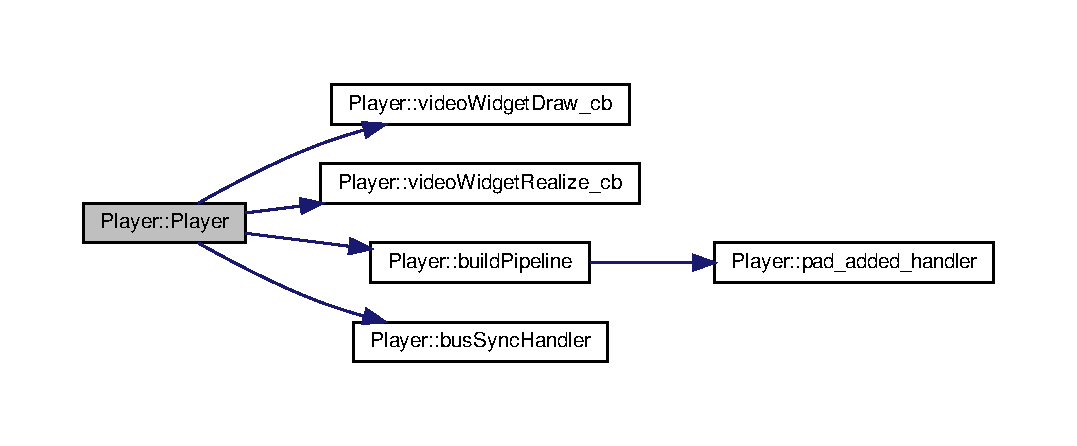
\includegraphics[width=350pt]{class_player_a0e17f3ec3397aa056d2ee88a060a7d36_cgraph}
\end{center}
\end{figure}
\mbox{\Hypertarget{class_player_a749d2c00e1fe0f5c2746f7505a58c062}\label{class_player_a749d2c00e1fe0f5c2746f7505a58c062}} 
\index{Player@{Player}!````~Player@{$\sim$\+Player}}
\index{````~Player@{$\sim$\+Player}!Player@{Player}}
\subsubsection{\texorpdfstring{$\sim$\+Player()}{~Player()}\hspace{0.1cm}{\footnotesize\ttfamily [1/2]}}
{\footnotesize\ttfamily Player\+::$\sim$\+Player (\begin{DoxyParamCaption}{ }\end{DoxyParamCaption})}

\mbox{\Hypertarget{class_player_a4b179b1c59f780f59e215fa5642acb99}\label{class_player_a4b179b1c59f780f59e215fa5642acb99}} 
\index{Player@{Player}!Player@{Player}}
\index{Player@{Player}!Player@{Player}}
\subsubsection{\texorpdfstring{Player()}{Player()}\hspace{0.1cm}{\footnotesize\ttfamily [2/2]}}
{\footnotesize\ttfamily Player\+::\+Player (\begin{DoxyParamCaption}\item[{Gtk\+Widget $\ast$}]{video\+Window,  }\item[{\hyperlink{class_config}{Config} $\ast$}]{config }\end{DoxyParamCaption})}

Граф вызовов\+:\nopagebreak
\begin{figure}[H]
\begin{center}
\leavevmode
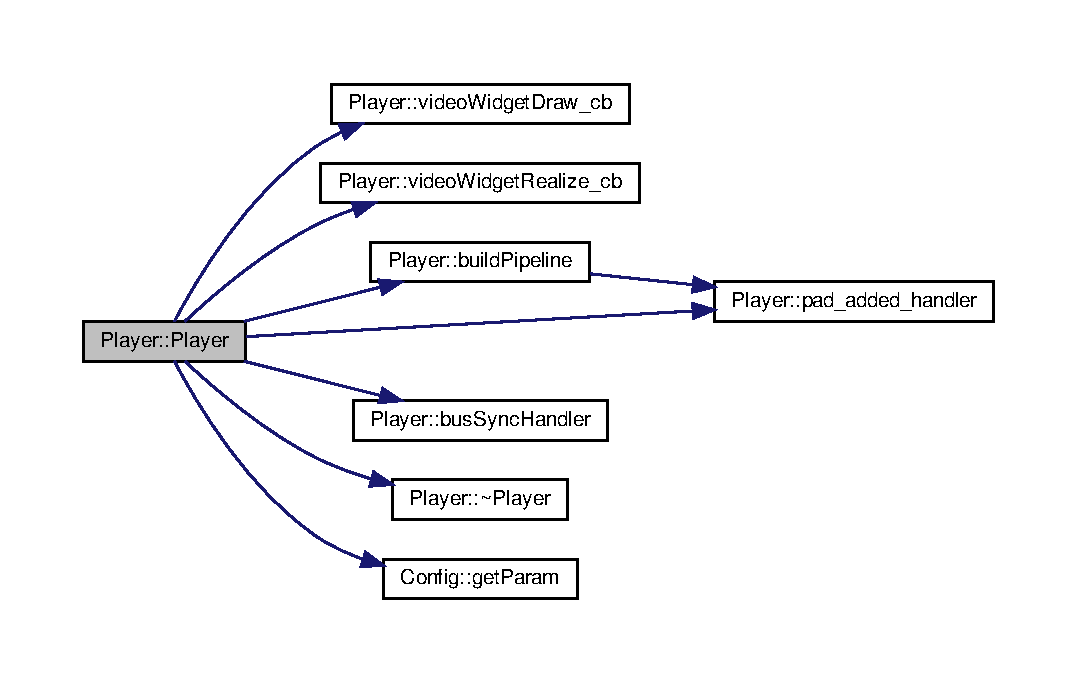
\includegraphics[width=350pt]{class_player_a4b179b1c59f780f59e215fa5642acb99_cgraph}
\end{center}
\end{figure}
\mbox{\Hypertarget{class_player_a749d2c00e1fe0f5c2746f7505a58c062}\label{class_player_a749d2c00e1fe0f5c2746f7505a58c062}} 
\index{Player@{Player}!````~Player@{$\sim$\+Player}}
\index{````~Player@{$\sim$\+Player}!Player@{Player}}
\subsubsection{\texorpdfstring{$\sim$\+Player()}{~Player()}\hspace{0.1cm}{\footnotesize\ttfamily [2/2]}}
{\footnotesize\ttfamily Player\+::$\sim$\+Player (\begin{DoxyParamCaption}{ }\end{DoxyParamCaption})}



\subsection{Методы}
\mbox{\Hypertarget{class_player_aca2616201a97a901612fd9df7a900ca1}\label{class_player_aca2616201a97a901612fd9df7a900ca1}} 
\index{Player@{Player}!build\+Pipeline@{build\+Pipeline}}
\index{build\+Pipeline@{build\+Pipeline}!Player@{Player}}
\subsubsection{\texorpdfstring{build\+Pipeline()}{buildPipeline()}\hspace{0.1cm}{\footnotesize\ttfamily [1/2]}}
{\footnotesize\ttfamily void Player\+::build\+Pipeline (\begin{DoxyParamCaption}{ }\end{DoxyParamCaption})\hspace{0.3cm}{\ttfamily [private]}}

\mbox{\Hypertarget{class_player_aca2616201a97a901612fd9df7a900ca1}\label{class_player_aca2616201a97a901612fd9df7a900ca1}} 
\index{Player@{Player}!build\+Pipeline@{build\+Pipeline}}
\index{build\+Pipeline@{build\+Pipeline}!Player@{Player}}
\subsubsection{\texorpdfstring{build\+Pipeline()}{buildPipeline()}\hspace{0.1cm}{\footnotesize\ttfamily [2/2]}}
{\footnotesize\ttfamily void Player\+::build\+Pipeline (\begin{DoxyParamCaption}{ }\end{DoxyParamCaption})\hspace{0.3cm}{\ttfamily [private]}}

Граф вызовов\+:\nopagebreak
\begin{figure}[H]
\begin{center}
\leavevmode
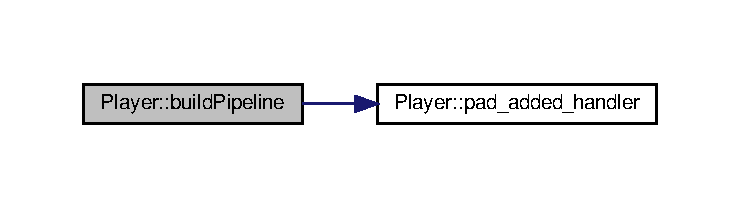
\includegraphics[width=350pt]{class_player_aca2616201a97a901612fd9df7a900ca1_cgraph}
\end{center}
\end{figure}
\mbox{\Hypertarget{class_player_a4f4e39756894a693bc45515f9eeded97}\label{class_player_a4f4e39756894a693bc45515f9eeded97}} 
\index{Player@{Player}!bus\+Sync\+Handler@{bus\+Sync\+Handler}}
\index{bus\+Sync\+Handler@{bus\+Sync\+Handler}!Player@{Player}}
\subsubsection{\texorpdfstring{bus\+Sync\+Handler()}{busSyncHandler()}\hspace{0.1cm}{\footnotesize\ttfamily [1/2]}}
{\footnotesize\ttfamily static Gst\+Bus\+Sync\+Reply Player\+::bus\+Sync\+Handler (\begin{DoxyParamCaption}\item[{Gst\+Bus $\ast$}]{bus,  }\item[{Gst\+Message $\ast$}]{message,  }\item[{\hyperlink{class_player}{Player} $\ast$}]{player }\end{DoxyParamCaption})\hspace{0.3cm}{\ttfamily [static]}, {\ttfamily [private]}}

\mbox{\Hypertarget{class_player_a987a5a6f6bf24f530536090e9a832ef6}\label{class_player_a987a5a6f6bf24f530536090e9a832ef6}} 
\index{Player@{Player}!bus\+Sync\+Handler@{bus\+Sync\+Handler}}
\index{bus\+Sync\+Handler@{bus\+Sync\+Handler}!Player@{Player}}
\subsubsection{\texorpdfstring{bus\+Sync\+Handler()}{busSyncHandler()}\hspace{0.1cm}{\footnotesize\ttfamily [2/2]}}
{\footnotesize\ttfamily Gst\+Bus\+Sync\+Reply Player\+::bus\+Sync\+Handler (\begin{DoxyParamCaption}\item[{Gst\+Bus $\ast$}]{bus,  }\item[{Gst\+Message $\ast$}]{message,  }\item[{\hyperlink{class_player}{Player} $\ast$}]{player }\end{DoxyParamCaption})\hspace{0.3cm}{\ttfamily [static]}, {\ttfamily [private]}}

\mbox{\Hypertarget{class_player_a370339dfdf9eb61905637283a72f9e22}\label{class_player_a370339dfdf9eb61905637283a72f9e22}} 
\index{Player@{Player}!is\+Playing@{is\+Playing}}
\index{is\+Playing@{is\+Playing}!Player@{Player}}
\subsubsection{\texorpdfstring{is\+Playing()}{isPlaying()}}
{\footnotesize\ttfamily bool Player\+::is\+Playing (\begin{DoxyParamCaption}{ }\end{DoxyParamCaption})\hspace{0.3cm}{\ttfamily [inline]}}

\mbox{\Hypertarget{class_player_a3e74802e5bf9b62f5a0908637ace1913}\label{class_player_a3e74802e5bf9b62f5a0908637ace1913}} 
\index{Player@{Player}!pad\+\_\+added\+\_\+handler@{pad\+\_\+added\+\_\+handler}}
\index{pad\+\_\+added\+\_\+handler@{pad\+\_\+added\+\_\+handler}!Player@{Player}}
\subsubsection{\texorpdfstring{pad\+\_\+added\+\_\+handler()}{pad\_added\_handler()}\hspace{0.1cm}{\footnotesize\ttfamily [1/2]}}
{\footnotesize\ttfamily static void Player\+::pad\+\_\+added\+\_\+handler (\begin{DoxyParamCaption}\item[{Gst\+Element $\ast$}]{src,  }\item[{Gst\+Pad $\ast$}]{new\+\_\+pad,  }\item[{\hyperlink{class_player}{Player} $\ast$}]{player }\end{DoxyParamCaption})\hspace{0.3cm}{\ttfamily [static]}, {\ttfamily [private]}}

\mbox{\Hypertarget{class_player_a43527d455f9de17468deb13fef887854}\label{class_player_a43527d455f9de17468deb13fef887854}} 
\index{Player@{Player}!pad\+\_\+added\+\_\+handler@{pad\+\_\+added\+\_\+handler}}
\index{pad\+\_\+added\+\_\+handler@{pad\+\_\+added\+\_\+handler}!Player@{Player}}
\subsubsection{\texorpdfstring{pad\+\_\+added\+\_\+handler()}{pad\_added\_handler()}\hspace{0.1cm}{\footnotesize\ttfamily [2/2]}}
{\footnotesize\ttfamily void Player\+::pad\+\_\+added\+\_\+handler (\begin{DoxyParamCaption}\item[{Gst\+Element $\ast$}]{src,  }\item[{Gst\+Pad $\ast$}]{new\+\_\+pad,  }\item[{\hyperlink{class_player}{Player} $\ast$}]{player }\end{DoxyParamCaption})\hspace{0.3cm}{\ttfamily [static]}, {\ttfamily [private]}}

\mbox{\Hypertarget{class_player_a75c7257813c5f96bb2d8585dfc0c3025}\label{class_player_a75c7257813c5f96bb2d8585dfc0c3025}} 
\index{Player@{Player}!play\+Stream@{play\+Stream}}
\index{play\+Stream@{play\+Stream}!Player@{Player}}
\subsubsection{\texorpdfstring{play\+Stream()}{playStream()}\hspace{0.1cm}{\footnotesize\ttfamily [1/2]}}
{\footnotesize\ttfamily void Player\+::play\+Stream (\begin{DoxyParamCaption}\item[{string}]{uri }\end{DoxyParamCaption})}

Граф вызовов\+:\nopagebreak
\begin{figure}[H]
\begin{center}
\leavevmode
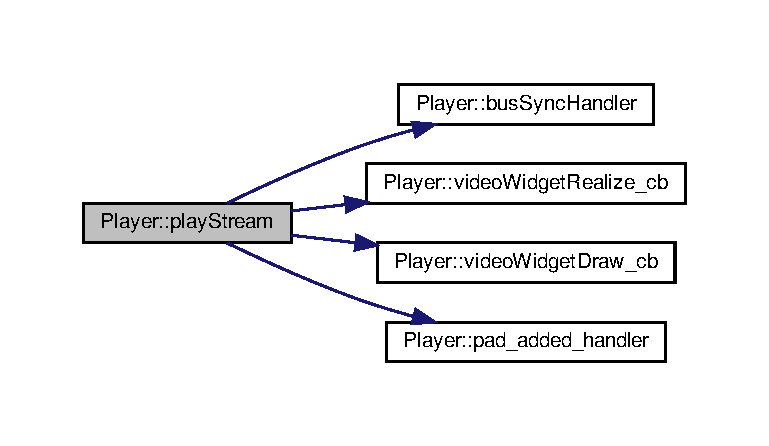
\includegraphics[width=350pt]{class_player_a75c7257813c5f96bb2d8585dfc0c3025_cgraph}
\end{center}
\end{figure}
\mbox{\Hypertarget{class_player_a082180138fe92098aa9a1f51fd9ad40d}\label{class_player_a082180138fe92098aa9a1f51fd9ad40d}} 
\index{Player@{Player}!play\+Stream@{play\+Stream}}
\index{play\+Stream@{play\+Stream}!Player@{Player}}
\subsubsection{\texorpdfstring{play\+Stream()}{playStream()}\hspace{0.1cm}{\footnotesize\ttfamily [2/2]}}
{\footnotesize\ttfamily void Player\+::play\+Stream (\begin{DoxyParamCaption}{ }\end{DoxyParamCaption})}

\mbox{\Hypertarget{class_player_aa8396672dd38d93e1000b7b0f55e9c24}\label{class_player_aa8396672dd38d93e1000b7b0f55e9c24}} 
\index{Player@{Player}!stop\+Stream@{stop\+Stream}}
\index{stop\+Stream@{stop\+Stream}!Player@{Player}}
\subsubsection{\texorpdfstring{stop\+Stream()}{stopStream()}}
{\footnotesize\ttfamily void Player\+::stop\+Stream (\begin{DoxyParamCaption}{ }\end{DoxyParamCaption})}

\mbox{\Hypertarget{class_player_a3e6f827b42b56e7685a66e739d643ecc}\label{class_player_a3e6f827b42b56e7685a66e739d643ecc}} 
\index{Player@{Player}!video\+Widget\+Draw\+\_\+cb@{video\+Widget\+Draw\+\_\+cb}}
\index{video\+Widget\+Draw\+\_\+cb@{video\+Widget\+Draw\+\_\+cb}!Player@{Player}}
\subsubsection{\texorpdfstring{video\+Widget\+Draw\+\_\+cb()}{videoWidgetDraw\_cb()}\hspace{0.1cm}{\footnotesize\ttfamily [1/2]}}
{\footnotesize\ttfamily static gboolean Player\+::video\+Widget\+Draw\+\_\+cb (\begin{DoxyParamCaption}\item[{Gtk\+Widget $\ast$}]{widget,  }\item[{cairo\+\_\+t $\ast$}]{cr,  }\item[{gpointer}]{user\+\_\+data }\end{DoxyParamCaption})\hspace{0.3cm}{\ttfamily [static]}, {\ttfamily [private]}}

\mbox{\Hypertarget{class_player_a31a79db48e8ebebddacd1bd76bf16f3d}\label{class_player_a31a79db48e8ebebddacd1bd76bf16f3d}} 
\index{Player@{Player}!video\+Widget\+Draw\+\_\+cb@{video\+Widget\+Draw\+\_\+cb}}
\index{video\+Widget\+Draw\+\_\+cb@{video\+Widget\+Draw\+\_\+cb}!Player@{Player}}
\subsubsection{\texorpdfstring{video\+Widget\+Draw\+\_\+cb()}{videoWidgetDraw\_cb()}\hspace{0.1cm}{\footnotesize\ttfamily [2/2]}}
{\footnotesize\ttfamily gboolean Player\+::video\+Widget\+Draw\+\_\+cb (\begin{DoxyParamCaption}\item[{Gtk\+Widget $\ast$}]{widget,  }\item[{cairo\+\_\+t $\ast$}]{cr,  }\item[{gpointer}]{user\+\_\+data }\end{DoxyParamCaption})\hspace{0.3cm}{\ttfamily [static]}, {\ttfamily [private]}}

\mbox{\Hypertarget{class_player_a6a18c90131b03493e506d50d16925436}\label{class_player_a6a18c90131b03493e506d50d16925436}} 
\index{Player@{Player}!video\+Widget\+Realize\+\_\+cb@{video\+Widget\+Realize\+\_\+cb}}
\index{video\+Widget\+Realize\+\_\+cb@{video\+Widget\+Realize\+\_\+cb}!Player@{Player}}
\subsubsection{\texorpdfstring{video\+Widget\+Realize\+\_\+cb()}{videoWidgetRealize\_cb()}\hspace{0.1cm}{\footnotesize\ttfamily [1/2]}}
{\footnotesize\ttfamily static void Player\+::video\+Widget\+Realize\+\_\+cb (\begin{DoxyParamCaption}\item[{Gtk\+Widget $\ast$}]{widget,  }\item[{\hyperlink{class_player}{Player} $\ast$}]{player }\end{DoxyParamCaption})\hspace{0.3cm}{\ttfamily [static]}, {\ttfamily [private]}}

\mbox{\Hypertarget{class_player_aeb024ba54089ecaf90753a6f6b8d07bc}\label{class_player_aeb024ba54089ecaf90753a6f6b8d07bc}} 
\index{Player@{Player}!video\+Widget\+Realize\+\_\+cb@{video\+Widget\+Realize\+\_\+cb}}
\index{video\+Widget\+Realize\+\_\+cb@{video\+Widget\+Realize\+\_\+cb}!Player@{Player}}
\subsubsection{\texorpdfstring{video\+Widget\+Realize\+\_\+cb()}{videoWidgetRealize\_cb()}\hspace{0.1cm}{\footnotesize\ttfamily [2/2]}}
{\footnotesize\ttfamily void Player\+::video\+Widget\+Realize\+\_\+cb (\begin{DoxyParamCaption}\item[{Gtk\+Widget $\ast$}]{widget,  }\item[{\hyperlink{class_player}{Player} $\ast$}]{player }\end{DoxyParamCaption})\hspace{0.3cm}{\ttfamily [static]}, {\ttfamily [private]}}



\subsection{Данные класса}
\mbox{\Hypertarget{class_player_a746993d3cf67692b460334b0e0ede459}\label{class_player_a746993d3cf67692b460334b0e0ede459}} 
\index{Player@{Player}!bus@{bus}}
\index{bus@{bus}!Player@{Player}}
\subsubsection{\texorpdfstring{bus}{bus}}
{\footnotesize\ttfamily Gst\+Bus $\ast$ Player\+::bus\hspace{0.3cm}{\ttfamily [private]}}

\mbox{\Hypertarget{class_player_af5647b79bedfd422ca8758c90c6bbc45}\label{class_player_af5647b79bedfd422ca8758c90c6bbc45}} 
\index{Player@{Player}!cam\+Name@{cam\+Name}}
\index{cam\+Name@{cam\+Name}!Player@{Player}}
\subsubsection{\texorpdfstring{cam\+Name}{camName}}
{\footnotesize\ttfamily string Player\+::cam\+Name\hspace{0.3cm}{\ttfamily [private]}}

\mbox{\Hypertarget{class_player_a53cd9b524dac60ecacd99f0812c71332}\label{class_player_a53cd9b524dac60ecacd99f0812c71332}} 
\index{Player@{Player}!config@{config}}
\index{config@{config}!Player@{Player}}
\subsubsection{\texorpdfstring{config}{config}}
{\footnotesize\ttfamily \hyperlink{class_config}{Config}$\ast$ Player\+::config}

\mbox{\Hypertarget{class_player_a79ccb8bdee134c230a8c242d5123356d}\label{class_player_a79ccb8bdee134c230a8c242d5123356d}} 
\index{Player@{Player}!dec@{dec}}
\index{dec@{dec}!Player@{Player}}
\subsubsection{\texorpdfstring{dec}{dec}}
{\footnotesize\ttfamily Gst\+Element $\ast$ Player\+::dec}

\mbox{\Hypertarget{class_player_a612fee9ac56aee91fd64e770f946e2e4}\label{class_player_a612fee9ac56aee91fd64e770f946e2e4}} 
\index{Player@{Player}!depay@{depay}}
\index{depay@{depay}!Player@{Player}}
\subsubsection{\texorpdfstring{depay}{depay}}
{\footnotesize\ttfamily Gst\+Element $\ast$ Player\+::depay}

\mbox{\Hypertarget{class_player_a9aafd7f61221255c78b81c8715148676}\label{class_player_a9aafd7f61221255c78b81c8715148676}} 
\index{Player@{Player}!parse@{parse}}
\index{parse@{parse}!Player@{Player}}
\subsubsection{\texorpdfstring{parse}{parse}}
{\footnotesize\ttfamily Gst\+Element $\ast$ Player\+::parse}

\mbox{\Hypertarget{class_player_aa8cd0e05525fd7cf5ee60b40b1388254}\label{class_player_aa8cd0e05525fd7cf5ee60b40b1388254}} 
\index{Player@{Player}!pipeline@{pipeline}}
\index{pipeline@{pipeline}!Player@{Player}}
\subsubsection{\texorpdfstring{pipeline}{pipeline}}
{\footnotesize\ttfamily Gst\+Element $\ast$ Player\+::pipeline}

\mbox{\Hypertarget{class_player_a4335f10f38749272bbdee425e8e30388}\label{class_player_a4335f10f38749272bbdee425e8e30388}} 
\index{Player@{Player}!platform@{platform}}
\index{platform@{platform}!Player@{Player}}
\subsubsection{\texorpdfstring{platform}{platform}}
{\footnotesize\ttfamily string Player\+::platform\hspace{0.3cm}{\ttfamily [private]}}

\mbox{\Hypertarget{class_player_a93eaebe50e6ab8a19c35138b4c60f60c}\label{class_player_a93eaebe50e6ab8a19c35138b4c60f60c}} 
\index{Player@{Player}!playing@{playing}}
\index{playing@{playing}!Player@{Player}}
\subsubsection{\texorpdfstring{playing}{playing}}
{\footnotesize\ttfamily bool Player\+::playing\hspace{0.3cm}{\ttfamily [private]}}

\mbox{\Hypertarget{class_player_a0cb0a126d4348e773fd2627c2a25d9e1}\label{class_player_a0cb0a126d4348e773fd2627c2a25d9e1}} 
\index{Player@{Player}!scale@{scale}}
\index{scale@{scale}!Player@{Player}}
\subsubsection{\texorpdfstring{scale}{scale}}
{\footnotesize\ttfamily Gst\+Element $\ast$ Player\+::scale}

\mbox{\Hypertarget{class_player_aabd00fa1e998c6e4db1a83e6fee285ba}\label{class_player_aabd00fa1e998c6e4db1a83e6fee285ba}} 
\index{Player@{Player}!sink@{sink}}
\index{sink@{sink}!Player@{Player}}
\subsubsection{\texorpdfstring{sink}{sink}}
{\footnotesize\ttfamily Gst\+Element $\ast$ Player\+::sink}

\mbox{\Hypertarget{class_player_ac3fb217cb2001134249fafcba07fe7e7}\label{class_player_ac3fb217cb2001134249fafcba07fe7e7}} 
\index{Player@{Player}!src@{src}}
\index{src@{src}!Player@{Player}}
\subsubsection{\texorpdfstring{src}{src}}
{\footnotesize\ttfamily Gst\+Element $\ast$ Player\+::src}

\mbox{\Hypertarget{class_player_a02eaaec54dce5238f76ef6b9f458c86d}\label{class_player_a02eaaec54dce5238f76ef6b9f458c86d}} 
\index{Player@{Player}!uri@{uri}}
\index{uri@{uri}!Player@{Player}}
\subsubsection{\texorpdfstring{uri}{uri}}
{\footnotesize\ttfamily string Player\+::uri\hspace{0.3cm}{\ttfamily [private]}}

\mbox{\Hypertarget{class_player_ae5ed3420e43869788a3e9bf4eb29e529}\label{class_player_ae5ed3420e43869788a3e9bf4eb29e529}} 
\index{Player@{Player}!video\+Window@{video\+Window}}
\index{video\+Window@{video\+Window}!Player@{Player}}
\subsubsection{\texorpdfstring{video\+Window}{videoWindow}}
{\footnotesize\ttfamily Gtk\+Widget $\ast$ Player\+::video\+Window\hspace{0.3cm}{\ttfamily [private]}}

\mbox{\Hypertarget{class_player_a6375b319e5ba03a025aea4a91f36f7eb}\label{class_player_a6375b319e5ba03a025aea4a91f36f7eb}} 
\index{Player@{Player}!video\+Window\+Handle@{video\+Window\+Handle}}
\index{video\+Window\+Handle@{video\+Window\+Handle}!Player@{Player}}
\subsubsection{\texorpdfstring{video\+Window\+Handle}{videoWindowHandle}}
{\footnotesize\ttfamily guintptr Player\+::video\+Window\+Handle = 0\hspace{0.3cm}{\ttfamily [private]}}



Объявления и описания членов классов находятся в файлах\+:\begin{DoxyCompactItemize}
\item 
/home/jetson/controlroom/\+Studio/\+Operator/\+Grid/include/\hyperlink{_operator_2_grid_2include_2player_8h}{player.\+h}\item 
/home/jetson/controlroom/\+Studio/\+Operator/\+Grid/src/\hyperlink{_operator_2_grid_2src_2player_8cpp}{player.\+cpp}\end{DoxyCompactItemize}

\hypertarget{class_recorder}{}\section{Класс Recorder}
\label{class_recorder}\index{Recorder@{Recorder}}


Управляет процессом записи  




{\ttfamily \#include $<$recorder.\+h$>$}



Граф связей класса Recorder\+:\nopagebreak
\begin{figure}[H]
\begin{center}
\leavevmode
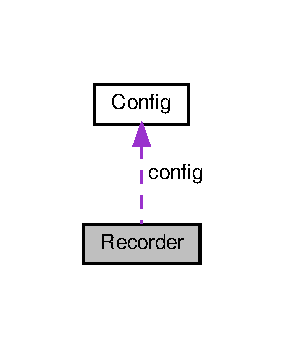
\includegraphics[width=138pt]{class_recorder__coll__graph}
\end{center}
\end{figure}
\subsection*{Открытые члены}
\begin{DoxyCompactItemize}
\item 
\hyperlink{class_recorder_aa3cf7e6df22a7a21e8939e1dc1d02ea1}{Recorder} (\hyperlink{class_config}{Config} $\ast$\hyperlink{class_recorder_acc5a095c1d30b547c994f817438c054b}{config})
\item 
\hyperlink{class_recorder_a6b3c569577fcdc298d8d4a6a2b96e9a9}{$\sim$\+Recorder} ()
\item 
map$<$ \hyperlink{struct_camera}{Camera} $\ast$, \hyperlink{class_recording}{Recording} $\ast$ $>$ \hyperlink{class_recorder_afb29e7ee1c1d78b3b2c9e54133f88b62}{get\+Running\+Recordings} ()
\item 
bool \hyperlink{class_recorder_ac242ca5967dbf81f9ea39464eee2b06a}{start\+Recording} (\hyperlink{struct_camera}{Camera} $\ast$cam)
\item 
bool \hyperlink{class_recorder_ae3de658eb341149ef0fb207783b3602b}{stop\+Recording} (\hyperlink{struct_camera}{Camera} $\ast$cam)
\item 
bool \hyperlink{class_recorder_a2c3f20dfa022c936ede65ca34becb890}{is\+G\+Drive\+Upload\+Active} ()
\end{DoxyCompactItemize}
\subsection*{Закрытые члены}
\begin{DoxyCompactItemize}
\item 
void \hyperlink{class_recorder_a2decf81333499f7c9f0193daed7e2091}{upload\+Video} (string uri, string file\+Name)
\end{DoxyCompactItemize}
\subsection*{Закрытые статические члены}
\begin{DoxyCompactItemize}
\item 
static gboolean \hyperlink{class_recorder_a1fdebd3d390713fcafe6c76635760841}{check\+If\+Rec\+Stopped} (gpointer data)
\end{DoxyCompactItemize}
\subsection*{Закрытые данные}
\begin{DoxyCompactItemize}
\item 
map$<$ \hyperlink{struct_camera}{Camera} $\ast$, \hyperlink{class_recording}{Recording} $\ast$ $>$ \hyperlink{class_recorder_a36bc2c958b17808861bd6f8b4204c82e}{running\+Recordings}
\item 
\hyperlink{class_config}{Config} $\ast$ \hyperlink{class_recorder_acc5a095c1d30b547c994f817438c054b}{config}
\item 
int \hyperlink{class_recorder_ae18bfd225286a1ebcd3b49de32d129cb}{running\+G\+Drive\+Uploads} = 0
\end{DoxyCompactItemize}


\subsection{Подробное описание}
Управляет процессом записи 

Forks gstreamer pipelines for each recording Needs a stream id to start a recording Stores pids of running recorder processes Stops recordings by stream id 

\subsection{Конструктор(ы)}
\mbox{\Hypertarget{class_recorder_aa3cf7e6df22a7a21e8939e1dc1d02ea1}\label{class_recorder_aa3cf7e6df22a7a21e8939e1dc1d02ea1}} 
\index{Recorder@{Recorder}!Recorder@{Recorder}}
\index{Recorder@{Recorder}!Recorder@{Recorder}}
\subsubsection{\texorpdfstring{Recorder()}{Recorder()}}
{\footnotesize\ttfamily Recorder\+::\+Recorder (\begin{DoxyParamCaption}\item[{\hyperlink{class_config}{Config} $\ast$}]{config }\end{DoxyParamCaption})}

Граф вызовов\+:\nopagebreak
\begin{figure}[H]
\begin{center}
\leavevmode
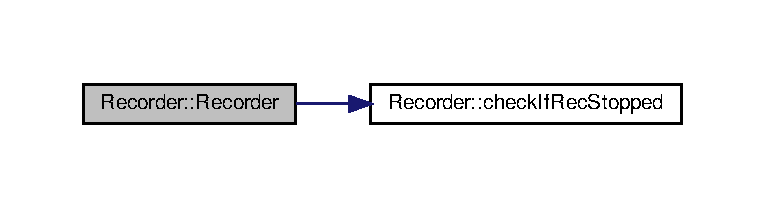
\includegraphics[width=350pt]{class_recorder_aa3cf7e6df22a7a21e8939e1dc1d02ea1_cgraph}
\end{center}
\end{figure}
\mbox{\Hypertarget{class_recorder_a6b3c569577fcdc298d8d4a6a2b96e9a9}\label{class_recorder_a6b3c569577fcdc298d8d4a6a2b96e9a9}} 
\index{Recorder@{Recorder}!````~Recorder@{$\sim$\+Recorder}}
\index{````~Recorder@{$\sim$\+Recorder}!Recorder@{Recorder}}
\subsubsection{\texorpdfstring{$\sim$\+Recorder()}{~Recorder()}}
{\footnotesize\ttfamily Recorder\+::$\sim$\+Recorder (\begin{DoxyParamCaption}{ }\end{DoxyParamCaption})}



\subsection{Методы}
\mbox{\Hypertarget{class_recorder_a1fdebd3d390713fcafe6c76635760841}\label{class_recorder_a1fdebd3d390713fcafe6c76635760841}} 
\index{Recorder@{Recorder}!check\+If\+Rec\+Stopped@{check\+If\+Rec\+Stopped}}
\index{check\+If\+Rec\+Stopped@{check\+If\+Rec\+Stopped}!Recorder@{Recorder}}
\subsubsection{\texorpdfstring{check\+If\+Rec\+Stopped()}{checkIfRecStopped()}}
{\footnotesize\ttfamily gboolean Recorder\+::check\+If\+Rec\+Stopped (\begin{DoxyParamCaption}\item[{gpointer}]{data }\end{DoxyParamCaption})\hspace{0.3cm}{\ttfamily [static]}, {\ttfamily [private]}}

\mbox{\Hypertarget{class_recorder_afb29e7ee1c1d78b3b2c9e54133f88b62}\label{class_recorder_afb29e7ee1c1d78b3b2c9e54133f88b62}} 
\index{Recorder@{Recorder}!get\+Running\+Recordings@{get\+Running\+Recordings}}
\index{get\+Running\+Recordings@{get\+Running\+Recordings}!Recorder@{Recorder}}
\subsubsection{\texorpdfstring{get\+Running\+Recordings()}{getRunningRecordings()}}
{\footnotesize\ttfamily map$<$\hyperlink{struct_camera}{Camera}$\ast$, \hyperlink{class_recording}{Recording}$\ast$$>$ Recorder\+::get\+Running\+Recordings (\begin{DoxyParamCaption}{ }\end{DoxyParamCaption})\hspace{0.3cm}{\ttfamily [inline]}}

\mbox{\Hypertarget{class_recorder_a2c3f20dfa022c936ede65ca34becb890}\label{class_recorder_a2c3f20dfa022c936ede65ca34becb890}} 
\index{Recorder@{Recorder}!is\+G\+Drive\+Upload\+Active@{is\+G\+Drive\+Upload\+Active}}
\index{is\+G\+Drive\+Upload\+Active@{is\+G\+Drive\+Upload\+Active}!Recorder@{Recorder}}
\subsubsection{\texorpdfstring{is\+G\+Drive\+Upload\+Active()}{isGDriveUploadActive()}}
{\footnotesize\ttfamily bool Recorder\+::is\+G\+Drive\+Upload\+Active (\begin{DoxyParamCaption}{ }\end{DoxyParamCaption})\hspace{0.3cm}{\ttfamily [inline]}}

\mbox{\Hypertarget{class_recorder_ac242ca5967dbf81f9ea39464eee2b06a}\label{class_recorder_ac242ca5967dbf81f9ea39464eee2b06a}} 
\index{Recorder@{Recorder}!start\+Recording@{start\+Recording}}
\index{start\+Recording@{start\+Recording}!Recorder@{Recorder}}
\subsubsection{\texorpdfstring{start\+Recording()}{startRecording()}}
{\footnotesize\ttfamily bool Recorder\+::start\+Recording (\begin{DoxyParamCaption}\item[{\hyperlink{struct_camera}{Camera} $\ast$}]{cam }\end{DoxyParamCaption})}

Граф вызовов\+:\nopagebreak
\begin{figure}[H]
\begin{center}
\leavevmode
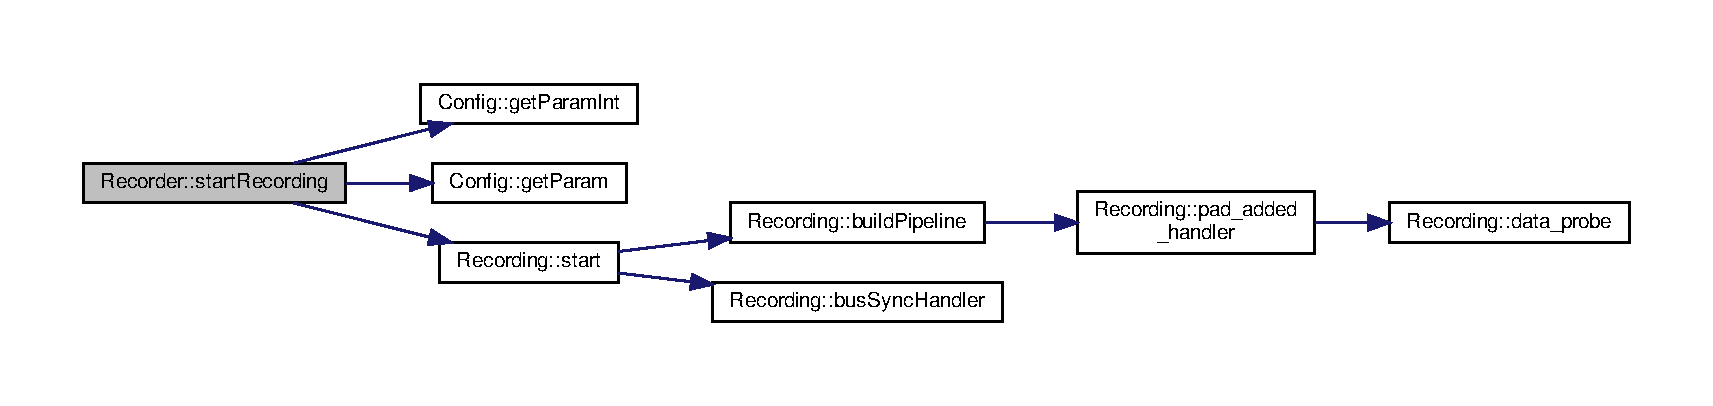
\includegraphics[width=350pt]{class_recorder_ac242ca5967dbf81f9ea39464eee2b06a_cgraph}
\end{center}
\end{figure}
\mbox{\Hypertarget{class_recorder_ae3de658eb341149ef0fb207783b3602b}\label{class_recorder_ae3de658eb341149ef0fb207783b3602b}} 
\index{Recorder@{Recorder}!stop\+Recording@{stop\+Recording}}
\index{stop\+Recording@{stop\+Recording}!Recorder@{Recorder}}
\subsubsection{\texorpdfstring{stop\+Recording()}{stopRecording()}}
{\footnotesize\ttfamily bool Recorder\+::stop\+Recording (\begin{DoxyParamCaption}\item[{\hyperlink{struct_camera}{Camera} $\ast$}]{cam }\end{DoxyParamCaption})}

\mbox{\Hypertarget{class_recorder_a2decf81333499f7c9f0193daed7e2091}\label{class_recorder_a2decf81333499f7c9f0193daed7e2091}} 
\index{Recorder@{Recorder}!upload\+Video@{upload\+Video}}
\index{upload\+Video@{upload\+Video}!Recorder@{Recorder}}
\subsubsection{\texorpdfstring{upload\+Video()}{uploadVideo()}}
{\footnotesize\ttfamily void Recorder\+::upload\+Video (\begin{DoxyParamCaption}\item[{string}]{uri,  }\item[{string}]{file\+Name }\end{DoxyParamCaption})\hspace{0.3cm}{\ttfamily [private]}}

Граф вызовов\+:\nopagebreak
\begin{figure}[H]
\begin{center}
\leavevmode
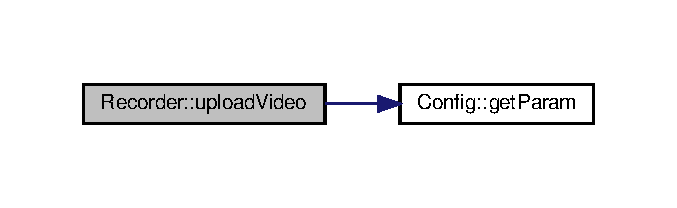
\includegraphics[width=325pt]{class_recorder_a2decf81333499f7c9f0193daed7e2091_cgraph}
\end{center}
\end{figure}


\subsection{Данные класса}
\mbox{\Hypertarget{class_recorder_acc5a095c1d30b547c994f817438c054b}\label{class_recorder_acc5a095c1d30b547c994f817438c054b}} 
\index{Recorder@{Recorder}!config@{config}}
\index{config@{config}!Recorder@{Recorder}}
\subsubsection{\texorpdfstring{config}{config}}
{\footnotesize\ttfamily \hyperlink{class_config}{Config}$\ast$ Recorder\+::config\hspace{0.3cm}{\ttfamily [private]}}

\mbox{\Hypertarget{class_recorder_ae18bfd225286a1ebcd3b49de32d129cb}\label{class_recorder_ae18bfd225286a1ebcd3b49de32d129cb}} 
\index{Recorder@{Recorder}!running\+G\+Drive\+Uploads@{running\+G\+Drive\+Uploads}}
\index{running\+G\+Drive\+Uploads@{running\+G\+Drive\+Uploads}!Recorder@{Recorder}}
\subsubsection{\texorpdfstring{running\+G\+Drive\+Uploads}{runningGDriveUploads}}
{\footnotesize\ttfamily int Recorder\+::running\+G\+Drive\+Uploads = 0\hspace{0.3cm}{\ttfamily [private]}}

\mbox{\Hypertarget{class_recorder_a36bc2c958b17808861bd6f8b4204c82e}\label{class_recorder_a36bc2c958b17808861bd6f8b4204c82e}} 
\index{Recorder@{Recorder}!running\+Recordings@{running\+Recordings}}
\index{running\+Recordings@{running\+Recordings}!Recorder@{Recorder}}
\subsubsection{\texorpdfstring{running\+Recordings}{runningRecordings}}
{\footnotesize\ttfamily map$<$\hyperlink{struct_camera}{Camera}$\ast$, \hyperlink{class_recording}{Recording}$\ast$$>$ Recorder\+::running\+Recordings\hspace{0.3cm}{\ttfamily [private]}}



Объявления и описания членов классов находятся в файлах\+:\begin{DoxyCompactItemize}
\item 
/home/jetson/controlroom/\+Studio/\+Recorder/include/\hyperlink{recorder_8h}{recorder.\+h}\item 
/home/jetson/controlroom/\+Studio/\+Recorder/src/\hyperlink{recorder_8cpp}{recorder.\+cpp}\end{DoxyCompactItemize}

\hypertarget{class_recording}{}\section{Класс Recording}
\label{class_recording}\index{Recording@{Recording}}


The \hyperlink{class_recording}{Recording} class.  




{\ttfamily \#include $<$recording.\+h$>$}

\subsection*{Открытые члены}
\begin{DoxyCompactItemize}
\item 
\hyperlink{class_recording_a128dd5017ad1bece8921226043c65fd7}{Recording} (string \hyperlink{class_recording_a60be340a7e3962c15362fb03d31dbba9}{uri}, string \hyperlink{class_recording_a0c0a828e5bf501fc26db662cb00dc6f4}{folder}, string \hyperlink{class_recording_a180143a05953b93dcc80707e36f4a282}{cam\+Name}, long \hyperlink{class_recording_a395293a5505e242ace2abd0ea8269d7c}{timeout}, long \hyperlink{class_recording_a222cf4edc0c19920121639525e6975e3}{video\+Time\+Limit})
\item 
\hyperlink{class_recording_a193bfe4e47869bec27433899dbe30543}{$\sim$\+Recording} ()
\item 
string \hyperlink{class_recording_a9c1a632374ab3887670ed1e9e18a5e50}{get\+File\+Name} ()
\item 
\hyperlink{recording_8h_af9bff8ff1154a04a899276af806b8586}{status\+\_\+t} \hyperlink{class_recording_a611b49ac3f6935c312a7f3dc141d3db7}{get\+Status} ()
\item 
bool \hyperlink{class_recording_a6258253b296dfc518b4c64c8f7cb9969}{start} ()
\item 
bool \hyperlink{class_recording_a1a53044e56c8a6cf6de62a9c0a7f9ae8}{stop} ()
\end{DoxyCompactItemize}
\subsection*{Открытые атрибуты}
\begin{DoxyCompactItemize}
\item 
\hyperlink{recording_8h_af9bff8ff1154a04a899276af806b8586}{status\+\_\+t} \hyperlink{class_recording_a607280d887f940ece786b3c1092739e7}{status}
\item 
string \hyperlink{class_recording_a60be340a7e3962c15362fb03d31dbba9}{uri}
\item 
string \hyperlink{class_recording_a180143a05953b93dcc80707e36f4a282}{cam\+Name}
\item 
string \hyperlink{class_recording_a01f00d2da7a894586da88ceed7c195d6}{file\+Name}
\item 
string \hyperlink{class_recording_a0c0a828e5bf501fc26db662cb00dc6f4}{folder}
\end{DoxyCompactItemize}
\subsection*{Закрытые члены}
\begin{DoxyCompactItemize}
\item 
bool \hyperlink{class_recording_a6fcee36a2d8276d6b7bc111800f41c49}{build\+Pipeline} ()
\end{DoxyCompactItemize}
\subsection*{Закрытые статические члены}
\begin{DoxyCompactItemize}
\item 
static void \hyperlink{class_recording_abea9877130d33f18639df0544497d473}{pad\+\_\+added\+\_\+handler} (Gst\+Element $\ast$\hyperlink{class_recording_ac8a63197a7a9f24e6af9d204c351d9ab}{src}, Gst\+Pad $\ast$new\+\_\+pad, \hyperlink{class_recording}{Recording} $\ast$recording)
\item 
static Gst\+Bus\+Sync\+Reply \hyperlink{class_recording_a902cb9d3bacaaf992e38427bbe63319b}{bus\+Sync\+Handler} (Gst\+Bus $\ast$bus, Gst\+Message $\ast$message, \hyperlink{class_recording}{Recording} $\ast$recording)
\item 
static Gst\+Pad\+Probe\+Return \hyperlink{class_recording_a60c63e897855daf4532e7a03c8a37026}{probe\+\_\+block\+\_\+stream} (Gst\+Pad $\ast$pad, Gst\+Pad\+Probe\+Info $\ast$info, gpointer user\+\_\+data)
\item 
static Gst\+Pad\+Probe\+Return \hyperlink{class_recording_a235992b4e8c358b6a648d84ed1e69969}{probe\+\_\+eos\+\_\+in\+\_\+stream} (Gst\+Pad $\ast$pad, Gst\+Pad\+Probe\+Info $\ast$info, gpointer user\+\_\+data)
\item 
static Gst\+Pad\+Probe\+Return \hyperlink{class_recording_a489e974a8481fdc9b6161c96f59ece8e}{probe\+\_\+idle\+\_\+relink} (Gst\+Pad $\ast$pad, Gst\+Pad\+Probe\+Info $\ast$info, gpointer user\+\_\+data)
\item 
static Gst\+Pad\+Probe\+Return \hyperlink{class_recording_aaff0d133af8cc8bc3f514b7ae85fc99a}{data\+\_\+probe} (Gst\+Pad $\ast$pad, Gst\+Pad\+Probe\+Info $\ast$info, gpointer user\+\_\+data)
\item 
static gboolean \hyperlink{class_recording_aebc44e786341582a88b0d91889110c3c}{freeze\+\_\+check} (gpointer user\+\_\+data)
\item 
static bool \hyperlink{class_recording_ab2a5a4db519db59f6de69699bfe04bc6}{element\+Src\+Linked} (Gst\+Element $\ast$elem)
\item 
static bool \hyperlink{class_recording_ac7f2d0b11324334fe3c54927fae60d9c}{element\+Sink\+Linked} (Gst\+Element $\ast$elem)
\item 
static bool \hyperlink{class_recording_a8cff139562008be79b2368c4a51d6ffe}{relink\+Elements} (Gst\+Element $\ast$wrong\+\_\+src, Gst\+Element $\ast$right\+\_\+src, Gst\+Element $\ast$\hyperlink{class_recording_a006ab2adce4204e46eea916f17b68401}{sink})
\end{DoxyCompactItemize}
\subsection*{Закрытые данные}
\begin{DoxyCompactItemize}
\item 
long \hyperlink{class_recording_a395293a5505e242ace2abd0ea8269d7c}{timeout}
\item 
long \hyperlink{class_recording_a222cf4edc0c19920121639525e6975e3}{video\+Time\+Limit}
\item 
int \hyperlink{class_recording_aef145697847a9e6675766dff249cf345}{freeze\+\_\+check\+\_\+id}
\item 
bool \hyperlink{class_recording_a8b3e718465495256436ee9dec586db1b}{stream\+Linked}
\item 
Gst\+Element $\ast$ \hyperlink{class_recording_af8c6df8e128533d6302e1f3bbaeac24b}{pipeline}
\item 
Gst\+Element $\ast$ \hyperlink{class_recording_ac8a63197a7a9f24e6af9d204c351d9ab}{src}
\item 
Gst\+Element $\ast$ \hyperlink{class_recording_a8899df1df3191c30d75d1318f12a9bec}{testsrc}
\item 
Gst\+Element $\ast$ \hyperlink{class_recording_a52bbcffe004812e90c5153c9051ba42e}{depay}
\item 
Gst\+Element $\ast$ \hyperlink{class_recording_af9bcc96225df8f1bf8fa33605b275656}{parse}
\item 
Gst\+Element $\ast$ \hyperlink{class_recording_a8c794a5feb7aa0584742584bbaca44fe}{streamcapsfilter}
\item 
Gst\+Element $\ast$ \hyperlink{class_recording_aa27843b1afce4572ab5bf4a910290b59}{mux}
\item 
Gst\+Element $\ast$ \hyperlink{class_recording_a006ab2adce4204e46eea916f17b68401}{sink}
\item 
Gst\+Element $\ast$ \hyperlink{class_recording_ab6006415906dfd17903df1bd5e45445c}{enc}
\item 
Gst\+Element $\ast$ \hyperlink{class_recording_ac94a1a97b8e08c825dcfb7a75b20dfed}{fakesink}
\item 
Gst\+Element $\ast$ \hyperlink{class_recording_aa947984714cd94e8648c51fed143059c}{testcapsfilter}
\item 
Gst\+Clock $\ast$ \hyperlink{class_recording_a54a3555942d7e9980c1dd6af64de05e0}{clock}
\item 
Gst\+Clock\+Time \hyperlink{class_recording_a3dfeb68c3b09bd72f332f466b6512448}{last\+Buffer\+Time}
\item 
gint \hyperlink{class_recording_a62a737d846719fb3d13cbfec4f2b7387}{in\+\_\+idle\+\_\+probe}
\end{DoxyCompactItemize}


\subsection{Подробное описание}
The \hyperlink{class_recording}{Recording} class. 

\subsection{Конструктор(ы)}
\mbox{\Hypertarget{class_recording_a128dd5017ad1bece8921226043c65fd7}\label{class_recording_a128dd5017ad1bece8921226043c65fd7}} 
\index{Recording@{Recording}!Recording@{Recording}}
\index{Recording@{Recording}!Recording@{Recording}}
\subsubsection{\texorpdfstring{Recording()}{Recording()}}
{\footnotesize\ttfamily Recording\+::\+Recording (\begin{DoxyParamCaption}\item[{string}]{uri,  }\item[{string}]{folder,  }\item[{string}]{cam\+Name,  }\item[{long}]{timeout,  }\item[{long}]{video\+Time\+Limit }\end{DoxyParamCaption})}

\mbox{\Hypertarget{class_recording_a193bfe4e47869bec27433899dbe30543}\label{class_recording_a193bfe4e47869bec27433899dbe30543}} 
\index{Recording@{Recording}!````~Recording@{$\sim$\+Recording}}
\index{````~Recording@{$\sim$\+Recording}!Recording@{Recording}}
\subsubsection{\texorpdfstring{$\sim$\+Recording()}{~Recording()}}
{\footnotesize\ttfamily Recording\+::$\sim$\+Recording (\begin{DoxyParamCaption}{ }\end{DoxyParamCaption})}



\subsection{Методы}
\mbox{\Hypertarget{class_recording_a6fcee36a2d8276d6b7bc111800f41c49}\label{class_recording_a6fcee36a2d8276d6b7bc111800f41c49}} 
\index{Recording@{Recording}!build\+Pipeline@{build\+Pipeline}}
\index{build\+Pipeline@{build\+Pipeline}!Recording@{Recording}}
\subsubsection{\texorpdfstring{build\+Pipeline()}{buildPipeline()}}
{\footnotesize\ttfamily bool Recording\+::build\+Pipeline (\begin{DoxyParamCaption}{ }\end{DoxyParamCaption})\hspace{0.3cm}{\ttfamily [private]}}

Граф вызовов\+:\nopagebreak
\begin{figure}[H]
\begin{center}
\leavevmode
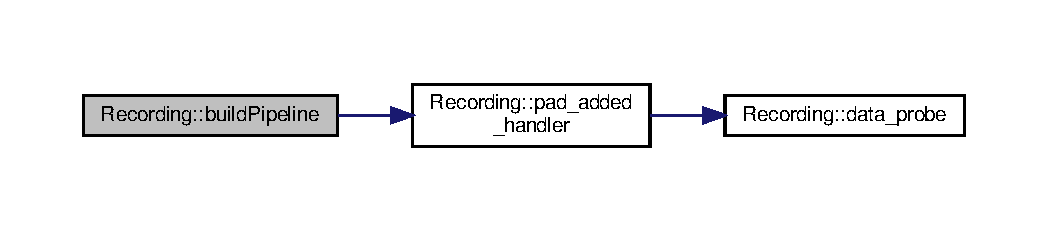
\includegraphics[width=350pt]{class_recording_a6fcee36a2d8276d6b7bc111800f41c49_cgraph}
\end{center}
\end{figure}
\mbox{\Hypertarget{class_recording_a902cb9d3bacaaf992e38427bbe63319b}\label{class_recording_a902cb9d3bacaaf992e38427bbe63319b}} 
\index{Recording@{Recording}!bus\+Sync\+Handler@{bus\+Sync\+Handler}}
\index{bus\+Sync\+Handler@{bus\+Sync\+Handler}!Recording@{Recording}}
\subsubsection{\texorpdfstring{bus\+Sync\+Handler()}{busSyncHandler()}}
{\footnotesize\ttfamily Gst\+Bus\+Sync\+Reply Recording\+::bus\+Sync\+Handler (\begin{DoxyParamCaption}\item[{Gst\+Bus $\ast$}]{bus,  }\item[{Gst\+Message $\ast$}]{message,  }\item[{\hyperlink{class_recording}{Recording} $\ast$}]{recording }\end{DoxyParamCaption})\hspace{0.3cm}{\ttfamily [static]}, {\ttfamily [private]}}

\mbox{\Hypertarget{class_recording_aaff0d133af8cc8bc3f514b7ae85fc99a}\label{class_recording_aaff0d133af8cc8bc3f514b7ae85fc99a}} 
\index{Recording@{Recording}!data\+\_\+probe@{data\+\_\+probe}}
\index{data\+\_\+probe@{data\+\_\+probe}!Recording@{Recording}}
\subsubsection{\texorpdfstring{data\+\_\+probe()}{data\_probe()}}
{\footnotesize\ttfamily Gst\+Pad\+Probe\+Return Recording\+::data\+\_\+probe (\begin{DoxyParamCaption}\item[{Gst\+Pad $\ast$}]{pad,  }\item[{Gst\+Pad\+Probe\+Info $\ast$}]{info,  }\item[{gpointer}]{user\+\_\+data }\end{DoxyParamCaption})\hspace{0.3cm}{\ttfamily [static]}, {\ttfamily [private]}}

\mbox{\Hypertarget{class_recording_ac7f2d0b11324334fe3c54927fae60d9c}\label{class_recording_ac7f2d0b11324334fe3c54927fae60d9c}} 
\index{Recording@{Recording}!element\+Sink\+Linked@{element\+Sink\+Linked}}
\index{element\+Sink\+Linked@{element\+Sink\+Linked}!Recording@{Recording}}
\subsubsection{\texorpdfstring{element\+Sink\+Linked()}{elementSinkLinked()}}
{\footnotesize\ttfamily bool Recording\+::element\+Sink\+Linked (\begin{DoxyParamCaption}\item[{Gst\+Element $\ast$}]{elem }\end{DoxyParamCaption})\hspace{0.3cm}{\ttfamily [static]}, {\ttfamily [private]}}

\mbox{\Hypertarget{class_recording_ab2a5a4db519db59f6de69699bfe04bc6}\label{class_recording_ab2a5a4db519db59f6de69699bfe04bc6}} 
\index{Recording@{Recording}!element\+Src\+Linked@{element\+Src\+Linked}}
\index{element\+Src\+Linked@{element\+Src\+Linked}!Recording@{Recording}}
\subsubsection{\texorpdfstring{element\+Src\+Linked()}{elementSrcLinked()}}
{\footnotesize\ttfamily bool Recording\+::element\+Src\+Linked (\begin{DoxyParamCaption}\item[{Gst\+Element $\ast$}]{elem }\end{DoxyParamCaption})\hspace{0.3cm}{\ttfamily [static]}, {\ttfamily [private]}}

\mbox{\Hypertarget{class_recording_aebc44e786341582a88b0d91889110c3c}\label{class_recording_aebc44e786341582a88b0d91889110c3c}} 
\index{Recording@{Recording}!freeze\+\_\+check@{freeze\+\_\+check}}
\index{freeze\+\_\+check@{freeze\+\_\+check}!Recording@{Recording}}
\subsubsection{\texorpdfstring{freeze\+\_\+check()}{freeze\_check()}}
{\footnotesize\ttfamily gboolean Recording\+::freeze\+\_\+check (\begin{DoxyParamCaption}\item[{gpointer}]{user\+\_\+data }\end{DoxyParamCaption})\hspace{0.3cm}{\ttfamily [static]}, {\ttfamily [private]}}

Граф вызовов\+:\nopagebreak
\begin{figure}[H]
\begin{center}
\leavevmode
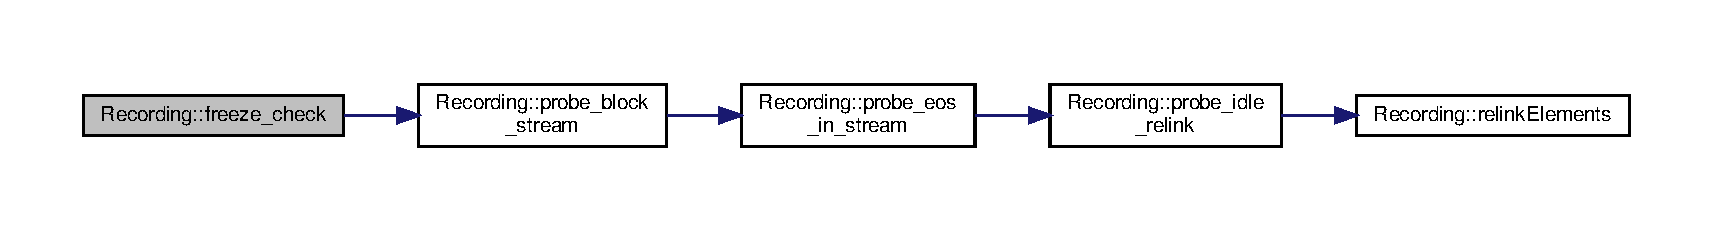
\includegraphics[width=350pt]{class_recording_aebc44e786341582a88b0d91889110c3c_cgraph}
\end{center}
\end{figure}
\mbox{\Hypertarget{class_recording_a9c1a632374ab3887670ed1e9e18a5e50}\label{class_recording_a9c1a632374ab3887670ed1e9e18a5e50}} 
\index{Recording@{Recording}!get\+File\+Name@{get\+File\+Name}}
\index{get\+File\+Name@{get\+File\+Name}!Recording@{Recording}}
\subsubsection{\texorpdfstring{get\+File\+Name()}{getFileName()}}
{\footnotesize\ttfamily string Recording\+::get\+File\+Name (\begin{DoxyParamCaption}{ }\end{DoxyParamCaption})\hspace{0.3cm}{\ttfamily [inline]}}

\mbox{\Hypertarget{class_recording_a611b49ac3f6935c312a7f3dc141d3db7}\label{class_recording_a611b49ac3f6935c312a7f3dc141d3db7}} 
\index{Recording@{Recording}!get\+Status@{get\+Status}}
\index{get\+Status@{get\+Status}!Recording@{Recording}}
\subsubsection{\texorpdfstring{get\+Status()}{getStatus()}}
{\footnotesize\ttfamily \hyperlink{recording_8h_af9bff8ff1154a04a899276af806b8586}{status\+\_\+t} Recording\+::get\+Status (\begin{DoxyParamCaption}{ }\end{DoxyParamCaption})\hspace{0.3cm}{\ttfamily [inline]}}

\mbox{\Hypertarget{class_recording_abea9877130d33f18639df0544497d473}\label{class_recording_abea9877130d33f18639df0544497d473}} 
\index{Recording@{Recording}!pad\+\_\+added\+\_\+handler@{pad\+\_\+added\+\_\+handler}}
\index{pad\+\_\+added\+\_\+handler@{pad\+\_\+added\+\_\+handler}!Recording@{Recording}}
\subsubsection{\texorpdfstring{pad\+\_\+added\+\_\+handler()}{pad\_added\_handler()}}
{\footnotesize\ttfamily void Recording\+::pad\+\_\+added\+\_\+handler (\begin{DoxyParamCaption}\item[{Gst\+Element $\ast$}]{src,  }\item[{Gst\+Pad $\ast$}]{new\+\_\+pad,  }\item[{\hyperlink{class_recording}{Recording} $\ast$}]{recording }\end{DoxyParamCaption})\hspace{0.3cm}{\ttfamily [static]}, {\ttfamily [private]}}

Граф вызовов\+:\nopagebreak
\begin{figure}[H]
\begin{center}
\leavevmode
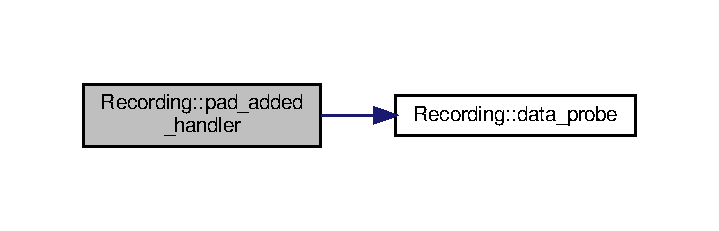
\includegraphics[width=345pt]{class_recording_abea9877130d33f18639df0544497d473_cgraph}
\end{center}
\end{figure}
\mbox{\Hypertarget{class_recording_a60c63e897855daf4532e7a03c8a37026}\label{class_recording_a60c63e897855daf4532e7a03c8a37026}} 
\index{Recording@{Recording}!probe\+\_\+block\+\_\+stream@{probe\+\_\+block\+\_\+stream}}
\index{probe\+\_\+block\+\_\+stream@{probe\+\_\+block\+\_\+stream}!Recording@{Recording}}
\subsubsection{\texorpdfstring{probe\+\_\+block\+\_\+stream()}{probe\_block\_stream()}}
{\footnotesize\ttfamily Gst\+Pad\+Probe\+Return Recording\+::probe\+\_\+block\+\_\+stream (\begin{DoxyParamCaption}\item[{Gst\+Pad $\ast$}]{pad,  }\item[{Gst\+Pad\+Probe\+Info $\ast$}]{info,  }\item[{gpointer}]{user\+\_\+data }\end{DoxyParamCaption})\hspace{0.3cm}{\ttfamily [static]}, {\ttfamily [private]}}

Граф вызовов\+:\nopagebreak
\begin{figure}[H]
\begin{center}
\leavevmode
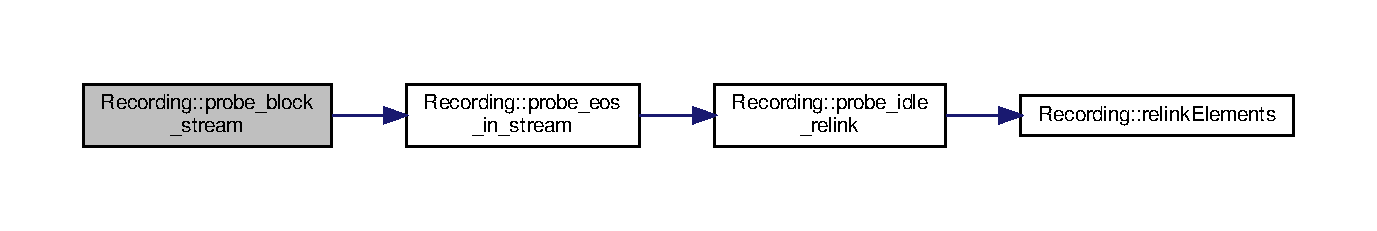
\includegraphics[width=350pt]{class_recording_a60c63e897855daf4532e7a03c8a37026_cgraph}
\end{center}
\end{figure}
\mbox{\Hypertarget{class_recording_a235992b4e8c358b6a648d84ed1e69969}\label{class_recording_a235992b4e8c358b6a648d84ed1e69969}} 
\index{Recording@{Recording}!probe\+\_\+eos\+\_\+in\+\_\+stream@{probe\+\_\+eos\+\_\+in\+\_\+stream}}
\index{probe\+\_\+eos\+\_\+in\+\_\+stream@{probe\+\_\+eos\+\_\+in\+\_\+stream}!Recording@{Recording}}
\subsubsection{\texorpdfstring{probe\+\_\+eos\+\_\+in\+\_\+stream()}{probe\_eos\_in\_stream()}}
{\footnotesize\ttfamily Gst\+Pad\+Probe\+Return Recording\+::probe\+\_\+eos\+\_\+in\+\_\+stream (\begin{DoxyParamCaption}\item[{Gst\+Pad $\ast$}]{pad,  }\item[{Gst\+Pad\+Probe\+Info $\ast$}]{info,  }\item[{gpointer}]{user\+\_\+data }\end{DoxyParamCaption})\hspace{0.3cm}{\ttfamily [static]}, {\ttfamily [private]}}

Граф вызовов\+:\nopagebreak
\begin{figure}[H]
\begin{center}
\leavevmode
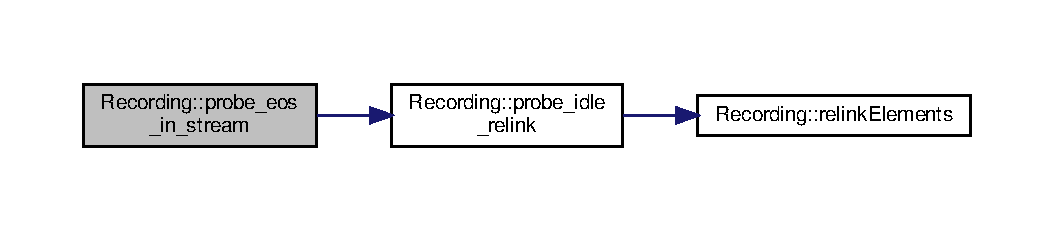
\includegraphics[width=350pt]{class_recording_a235992b4e8c358b6a648d84ed1e69969_cgraph}
\end{center}
\end{figure}
\mbox{\Hypertarget{class_recording_a489e974a8481fdc9b6161c96f59ece8e}\label{class_recording_a489e974a8481fdc9b6161c96f59ece8e}} 
\index{Recording@{Recording}!probe\+\_\+idle\+\_\+relink@{probe\+\_\+idle\+\_\+relink}}
\index{probe\+\_\+idle\+\_\+relink@{probe\+\_\+idle\+\_\+relink}!Recording@{Recording}}
\subsubsection{\texorpdfstring{probe\+\_\+idle\+\_\+relink()}{probe\_idle\_relink()}}
{\footnotesize\ttfamily Gst\+Pad\+Probe\+Return Recording\+::probe\+\_\+idle\+\_\+relink (\begin{DoxyParamCaption}\item[{Gst\+Pad $\ast$}]{pad,  }\item[{Gst\+Pad\+Probe\+Info $\ast$}]{info,  }\item[{gpointer}]{user\+\_\+data }\end{DoxyParamCaption})\hspace{0.3cm}{\ttfamily [static]}, {\ttfamily [private]}}

Граф вызовов\+:\nopagebreak
\begin{figure}[H]
\begin{center}
\leavevmode
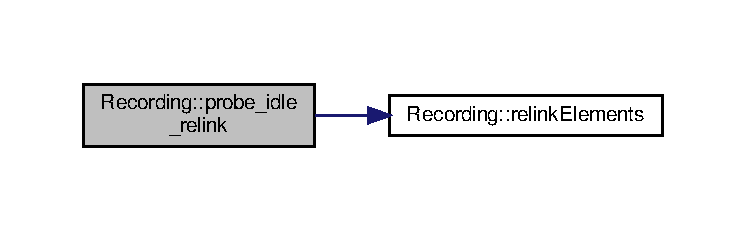
\includegraphics[width=350pt]{class_recording_a489e974a8481fdc9b6161c96f59ece8e_cgraph}
\end{center}
\end{figure}
\mbox{\Hypertarget{class_recording_a8cff139562008be79b2368c4a51d6ffe}\label{class_recording_a8cff139562008be79b2368c4a51d6ffe}} 
\index{Recording@{Recording}!relink\+Elements@{relink\+Elements}}
\index{relink\+Elements@{relink\+Elements}!Recording@{Recording}}
\subsubsection{\texorpdfstring{relink\+Elements()}{relinkElements()}}
{\footnotesize\ttfamily bool Recording\+::relink\+Elements (\begin{DoxyParamCaption}\item[{Gst\+Element $\ast$}]{wrong\+\_\+src,  }\item[{Gst\+Element $\ast$}]{right\+\_\+src,  }\item[{Gst\+Element $\ast$}]{sink }\end{DoxyParamCaption})\hspace{0.3cm}{\ttfamily [static]}, {\ttfamily [private]}}

\mbox{\Hypertarget{class_recording_a6258253b296dfc518b4c64c8f7cb9969}\label{class_recording_a6258253b296dfc518b4c64c8f7cb9969}} 
\index{Recording@{Recording}!start@{start}}
\index{start@{start}!Recording@{Recording}}
\subsubsection{\texorpdfstring{start()}{start()}}
{\footnotesize\ttfamily bool Recording\+::start (\begin{DoxyParamCaption}{ }\end{DoxyParamCaption})}

Граф вызовов\+:\nopagebreak
\begin{figure}[H]
\begin{center}
\leavevmode
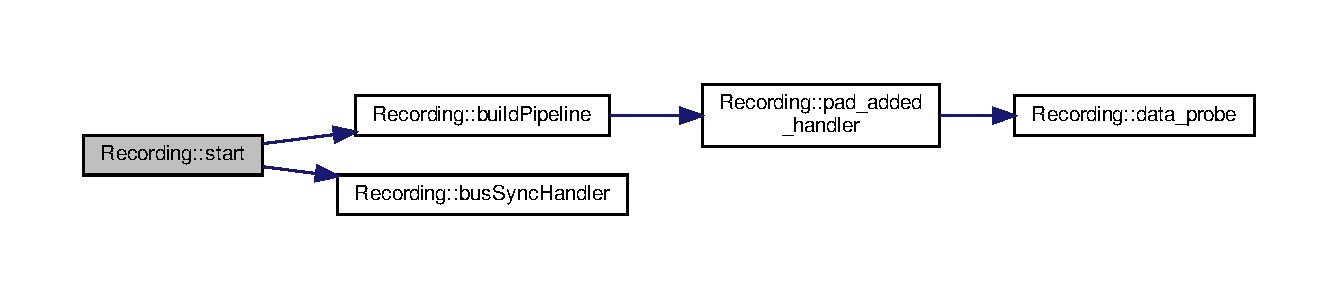
\includegraphics[width=350pt]{class_recording_a6258253b296dfc518b4c64c8f7cb9969_cgraph}
\end{center}
\end{figure}
\mbox{\Hypertarget{class_recording_a1a53044e56c8a6cf6de62a9c0a7f9ae8}\label{class_recording_a1a53044e56c8a6cf6de62a9c0a7f9ae8}} 
\index{Recording@{Recording}!stop@{stop}}
\index{stop@{stop}!Recording@{Recording}}
\subsubsection{\texorpdfstring{stop()}{stop()}}
{\footnotesize\ttfamily bool Recording\+::stop (\begin{DoxyParamCaption}{ }\end{DoxyParamCaption})}



\subsection{Данные класса}
\mbox{\Hypertarget{class_recording_a180143a05953b93dcc80707e36f4a282}\label{class_recording_a180143a05953b93dcc80707e36f4a282}} 
\index{Recording@{Recording}!cam\+Name@{cam\+Name}}
\index{cam\+Name@{cam\+Name}!Recording@{Recording}}
\subsubsection{\texorpdfstring{cam\+Name}{camName}}
{\footnotesize\ttfamily string Recording\+::cam\+Name}

\mbox{\Hypertarget{class_recording_a54a3555942d7e9980c1dd6af64de05e0}\label{class_recording_a54a3555942d7e9980c1dd6af64de05e0}} 
\index{Recording@{Recording}!clock@{clock}}
\index{clock@{clock}!Recording@{Recording}}
\subsubsection{\texorpdfstring{clock}{clock}}
{\footnotesize\ttfamily Gst\+Clock$\ast$ Recording\+::clock\hspace{0.3cm}{\ttfamily [private]}}

\mbox{\Hypertarget{class_recording_a52bbcffe004812e90c5153c9051ba42e}\label{class_recording_a52bbcffe004812e90c5153c9051ba42e}} 
\index{Recording@{Recording}!depay@{depay}}
\index{depay@{depay}!Recording@{Recording}}
\subsubsection{\texorpdfstring{depay}{depay}}
{\footnotesize\ttfamily Gst\+Element $\ast$ Recording\+::depay\hspace{0.3cm}{\ttfamily [private]}}

\mbox{\Hypertarget{class_recording_ab6006415906dfd17903df1bd5e45445c}\label{class_recording_ab6006415906dfd17903df1bd5e45445c}} 
\index{Recording@{Recording}!enc@{enc}}
\index{enc@{enc}!Recording@{Recording}}
\subsubsection{\texorpdfstring{enc}{enc}}
{\footnotesize\ttfamily Gst\+Element$\ast$ Recording\+::enc\hspace{0.3cm}{\ttfamily [private]}}

\mbox{\Hypertarget{class_recording_ac94a1a97b8e08c825dcfb7a75b20dfed}\label{class_recording_ac94a1a97b8e08c825dcfb7a75b20dfed}} 
\index{Recording@{Recording}!fakesink@{fakesink}}
\index{fakesink@{fakesink}!Recording@{Recording}}
\subsubsection{\texorpdfstring{fakesink}{fakesink}}
{\footnotesize\ttfamily Gst\+Element $\ast$ Recording\+::fakesink\hspace{0.3cm}{\ttfamily [private]}}

\mbox{\Hypertarget{class_recording_a01f00d2da7a894586da88ceed7c195d6}\label{class_recording_a01f00d2da7a894586da88ceed7c195d6}} 
\index{Recording@{Recording}!file\+Name@{file\+Name}}
\index{file\+Name@{file\+Name}!Recording@{Recording}}
\subsubsection{\texorpdfstring{file\+Name}{fileName}}
{\footnotesize\ttfamily string Recording\+::file\+Name}

\mbox{\Hypertarget{class_recording_a0c0a828e5bf501fc26db662cb00dc6f4}\label{class_recording_a0c0a828e5bf501fc26db662cb00dc6f4}} 
\index{Recording@{Recording}!folder@{folder}}
\index{folder@{folder}!Recording@{Recording}}
\subsubsection{\texorpdfstring{folder}{folder}}
{\footnotesize\ttfamily string Recording\+::folder}

\mbox{\Hypertarget{class_recording_aef145697847a9e6675766dff249cf345}\label{class_recording_aef145697847a9e6675766dff249cf345}} 
\index{Recording@{Recording}!freeze\+\_\+check\+\_\+id@{freeze\+\_\+check\+\_\+id}}
\index{freeze\+\_\+check\+\_\+id@{freeze\+\_\+check\+\_\+id}!Recording@{Recording}}
\subsubsection{\texorpdfstring{freeze\+\_\+check\+\_\+id}{freeze\_check\_id}}
{\footnotesize\ttfamily int Recording\+::freeze\+\_\+check\+\_\+id\hspace{0.3cm}{\ttfamily [private]}}

\mbox{\Hypertarget{class_recording_a62a737d846719fb3d13cbfec4f2b7387}\label{class_recording_a62a737d846719fb3d13cbfec4f2b7387}} 
\index{Recording@{Recording}!in\+\_\+idle\+\_\+probe@{in\+\_\+idle\+\_\+probe}}
\index{in\+\_\+idle\+\_\+probe@{in\+\_\+idle\+\_\+probe}!Recording@{Recording}}
\subsubsection{\texorpdfstring{in\+\_\+idle\+\_\+probe}{in\_idle\_probe}}
{\footnotesize\ttfamily gint Recording\+::in\+\_\+idle\+\_\+probe\hspace{0.3cm}{\ttfamily [private]}}

\mbox{\Hypertarget{class_recording_a3dfeb68c3b09bd72f332f466b6512448}\label{class_recording_a3dfeb68c3b09bd72f332f466b6512448}} 
\index{Recording@{Recording}!last\+Buffer\+Time@{last\+Buffer\+Time}}
\index{last\+Buffer\+Time@{last\+Buffer\+Time}!Recording@{Recording}}
\subsubsection{\texorpdfstring{last\+Buffer\+Time}{lastBufferTime}}
{\footnotesize\ttfamily Gst\+Clock\+Time Recording\+::last\+Buffer\+Time\hspace{0.3cm}{\ttfamily [private]}}

\mbox{\Hypertarget{class_recording_aa27843b1afce4572ab5bf4a910290b59}\label{class_recording_aa27843b1afce4572ab5bf4a910290b59}} 
\index{Recording@{Recording}!mux@{mux}}
\index{mux@{mux}!Recording@{Recording}}
\subsubsection{\texorpdfstring{mux}{mux}}
{\footnotesize\ttfamily Gst\+Element $\ast$ Recording\+::mux\hspace{0.3cm}{\ttfamily [private]}}

\mbox{\Hypertarget{class_recording_af9bcc96225df8f1bf8fa33605b275656}\label{class_recording_af9bcc96225df8f1bf8fa33605b275656}} 
\index{Recording@{Recording}!parse@{parse}}
\index{parse@{parse}!Recording@{Recording}}
\subsubsection{\texorpdfstring{parse}{parse}}
{\footnotesize\ttfamily Gst\+Element $\ast$ Recording\+::parse\hspace{0.3cm}{\ttfamily [private]}}

\mbox{\Hypertarget{class_recording_af8c6df8e128533d6302e1f3bbaeac24b}\label{class_recording_af8c6df8e128533d6302e1f3bbaeac24b}} 
\index{Recording@{Recording}!pipeline@{pipeline}}
\index{pipeline@{pipeline}!Recording@{Recording}}
\subsubsection{\texorpdfstring{pipeline}{pipeline}}
{\footnotesize\ttfamily Gst\+Element$\ast$ Recording\+::pipeline\hspace{0.3cm}{\ttfamily [private]}}

\mbox{\Hypertarget{class_recording_a006ab2adce4204e46eea916f17b68401}\label{class_recording_a006ab2adce4204e46eea916f17b68401}} 
\index{Recording@{Recording}!sink@{sink}}
\index{sink@{sink}!Recording@{Recording}}
\subsubsection{\texorpdfstring{sink}{sink}}
{\footnotesize\ttfamily Gst\+Element $\ast$ Recording\+::sink\hspace{0.3cm}{\ttfamily [private]}}

\mbox{\Hypertarget{class_recording_ac8a63197a7a9f24e6af9d204c351d9ab}\label{class_recording_ac8a63197a7a9f24e6af9d204c351d9ab}} 
\index{Recording@{Recording}!src@{src}}
\index{src@{src}!Recording@{Recording}}
\subsubsection{\texorpdfstring{src}{src}}
{\footnotesize\ttfamily Gst\+Element $\ast$ Recording\+::src\hspace{0.3cm}{\ttfamily [private]}}

\mbox{\Hypertarget{class_recording_a607280d887f940ece786b3c1092739e7}\label{class_recording_a607280d887f940ece786b3c1092739e7}} 
\index{Recording@{Recording}!status@{status}}
\index{status@{status}!Recording@{Recording}}
\subsubsection{\texorpdfstring{status}{status}}
{\footnotesize\ttfamily \hyperlink{recording_8h_af9bff8ff1154a04a899276af806b8586}{status\+\_\+t} Recording\+::status}

\mbox{\Hypertarget{class_recording_a8c794a5feb7aa0584742584bbaca44fe}\label{class_recording_a8c794a5feb7aa0584742584bbaca44fe}} 
\index{Recording@{Recording}!streamcapsfilter@{streamcapsfilter}}
\index{streamcapsfilter@{streamcapsfilter}!Recording@{Recording}}
\subsubsection{\texorpdfstring{streamcapsfilter}{streamcapsfilter}}
{\footnotesize\ttfamily Gst\+Element $\ast$ Recording\+::streamcapsfilter\hspace{0.3cm}{\ttfamily [private]}}

\mbox{\Hypertarget{class_recording_a8b3e718465495256436ee9dec586db1b}\label{class_recording_a8b3e718465495256436ee9dec586db1b}} 
\index{Recording@{Recording}!stream\+Linked@{stream\+Linked}}
\index{stream\+Linked@{stream\+Linked}!Recording@{Recording}}
\subsubsection{\texorpdfstring{stream\+Linked}{streamLinked}}
{\footnotesize\ttfamily bool Recording\+::stream\+Linked\hspace{0.3cm}{\ttfamily [private]}}

\mbox{\Hypertarget{class_recording_aa947984714cd94e8648c51fed143059c}\label{class_recording_aa947984714cd94e8648c51fed143059c}} 
\index{Recording@{Recording}!testcapsfilter@{testcapsfilter}}
\index{testcapsfilter@{testcapsfilter}!Recording@{Recording}}
\subsubsection{\texorpdfstring{testcapsfilter}{testcapsfilter}}
{\footnotesize\ttfamily Gst\+Element $\ast$ Recording\+::testcapsfilter\hspace{0.3cm}{\ttfamily [private]}}

\mbox{\Hypertarget{class_recording_a8899df1df3191c30d75d1318f12a9bec}\label{class_recording_a8899df1df3191c30d75d1318f12a9bec}} 
\index{Recording@{Recording}!testsrc@{testsrc}}
\index{testsrc@{testsrc}!Recording@{Recording}}
\subsubsection{\texorpdfstring{testsrc}{testsrc}}
{\footnotesize\ttfamily Gst\+Element $\ast$ Recording\+::testsrc\hspace{0.3cm}{\ttfamily [private]}}

\mbox{\Hypertarget{class_recording_a395293a5505e242ace2abd0ea8269d7c}\label{class_recording_a395293a5505e242ace2abd0ea8269d7c}} 
\index{Recording@{Recording}!timeout@{timeout}}
\index{timeout@{timeout}!Recording@{Recording}}
\subsubsection{\texorpdfstring{timeout}{timeout}}
{\footnotesize\ttfamily long Recording\+::timeout\hspace{0.3cm}{\ttfamily [private]}}

\mbox{\Hypertarget{class_recording_a60be340a7e3962c15362fb03d31dbba9}\label{class_recording_a60be340a7e3962c15362fb03d31dbba9}} 
\index{Recording@{Recording}!uri@{uri}}
\index{uri@{uri}!Recording@{Recording}}
\subsubsection{\texorpdfstring{uri}{uri}}
{\footnotesize\ttfamily string Recording\+::uri}

\mbox{\Hypertarget{class_recording_a222cf4edc0c19920121639525e6975e3}\label{class_recording_a222cf4edc0c19920121639525e6975e3}} 
\index{Recording@{Recording}!video\+Time\+Limit@{video\+Time\+Limit}}
\index{video\+Time\+Limit@{video\+Time\+Limit}!Recording@{Recording}}
\subsubsection{\texorpdfstring{video\+Time\+Limit}{videoTimeLimit}}
{\footnotesize\ttfamily long Recording\+::video\+Time\+Limit\hspace{0.3cm}{\ttfamily [private]}}



Объявления и описания членов классов находятся в файлах\+:\begin{DoxyCompactItemize}
\item 
/home/jetson/controlroom/\+Studio/\+Recorder/include/\hyperlink{recording_8h}{recording.\+h}\item 
/home/jetson/controlroom/\+Studio/\+Recorder/src/\hyperlink{recording_8cpp}{recording.\+cpp}\end{DoxyCompactItemize}

\hypertarget{class_room}{}\section{Класс Room}
\label{class_room}\index{Room@{Room}}


The \hyperlink{class_room}{Room} class.  




{\ttfamily \#include $<$room.\+h$>$}



Граф связей класса Room\+:\nopagebreak
\begin{figure}[H]
\begin{center}
\leavevmode
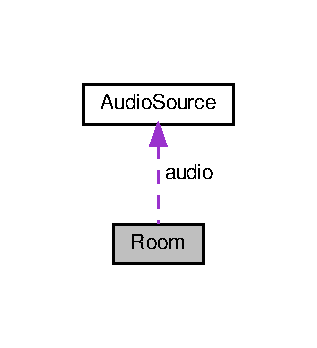
\includegraphics[width=152pt]{class_room__coll__graph}
\end{center}
\end{figure}
\subsection*{Открытые члены}
\begin{DoxyCompactItemize}
\item 
\hyperlink{class_room_a545e0b1d59ba66d72691c0dec993d9f0}{Room} (string \hyperlink{class_room_ae75204d685fe893bf4c867f9f3a79eb3}{name}, vector$<$ \hyperlink{struct_camera}{Camera} $>$ \hyperlink{class_room_a3e2ec3339b74eccacc2946d42151efc1}{cameras}, \hyperlink{struct_audio_source}{Audio\+Source} \hyperlink{class_room_a09874479cea41dde79c7c8dfdbd1703c}{audio})
\item 
\hyperlink{class_room_ac6ef93a7d9c3e1d624e025058d5f16ff}{Room} ()
\item 
string \hyperlink{class_room_a5701522ecf180c978eaa454d79f3e305}{get\+Name} ()
\item 
void \hyperlink{class_room_a3b4c4c8f33572ff196d75a187ed98021}{set\+Name} (string \hyperlink{class_room_ae75204d685fe893bf4c867f9f3a79eb3}{name})
\item 
vector$<$ \hyperlink{struct_camera}{Camera} $>$ $\ast$ \hyperlink{class_room_a4a67443ce377dda8f71d862428a31ef1}{get\+Cameras} ()
\item 
void \hyperlink{class_room_ae105a370ebb1cdded2254d39c547a5fd}{set\+Cameras} (vector$<$ \hyperlink{struct_camera}{Camera} $>$ cams)
\item 
\hyperlink{struct_audio_source}{Audio\+Source} \hyperlink{class_room_ad99b6c39b3322dc0f28ce31c35402bb9}{get\+Audio\+Source} ()
\item 
void \hyperlink{class_room_ae51a48335bf154e1194c1acc2fa16813}{set\+Audio\+Source} (\hyperlink{struct_audio_source}{Audio\+Source} \hyperlink{class_room_a09874479cea41dde79c7c8dfdbd1703c}{audio})
\item 
\hyperlink{class_room_a545e0b1d59ba66d72691c0dec993d9f0}{Room} (string \hyperlink{class_room_ae75204d685fe893bf4c867f9f3a79eb3}{name}, vector$<$ \hyperlink{struct_camera}{Camera} $>$ \hyperlink{class_room_a3e2ec3339b74eccacc2946d42151efc1}{cameras}, \hyperlink{struct_audio_source}{Audio\+Source} \hyperlink{class_room_a09874479cea41dde79c7c8dfdbd1703c}{audio})
\item 
\hyperlink{class_room_ac6ef93a7d9c3e1d624e025058d5f16ff}{Room} ()
\item 
string \hyperlink{class_room_a5701522ecf180c978eaa454d79f3e305}{get\+Name} ()
\item 
void \hyperlink{class_room_a3b4c4c8f33572ff196d75a187ed98021}{set\+Name} (string \hyperlink{class_room_ae75204d685fe893bf4c867f9f3a79eb3}{name})
\item 
vector$<$ \hyperlink{struct_camera}{Camera} $>$ $\ast$ \hyperlink{class_room_a4a67443ce377dda8f71d862428a31ef1}{get\+Cameras} ()
\item 
void \hyperlink{class_room_ae105a370ebb1cdded2254d39c547a5fd}{set\+Cameras} (vector$<$ \hyperlink{struct_camera}{Camera} $>$ cams)
\item 
\hyperlink{struct_audio_source}{Audio\+Source} \hyperlink{class_room_ad99b6c39b3322dc0f28ce31c35402bb9}{get\+Audio\+Source} ()
\item 
void \hyperlink{class_room_ae51a48335bf154e1194c1acc2fa16813}{set\+Audio\+Source} (\hyperlink{struct_audio_source}{Audio\+Source} \hyperlink{class_room_a09874479cea41dde79c7c8dfdbd1703c}{audio})
\end{DoxyCompactItemize}
\subsection*{Открытые атрибуты}
\begin{DoxyCompactItemize}
\item 
\hyperlink{_operator_2_grid_2include_2room_8h_aba46c5e77984ba564800a07427f8eeb1}{room\+\_\+t} \hyperlink{class_room_a9b8b36d17943edd1d8085bb5c2d8dbbf}{type}
\end{DoxyCompactItemize}
\subsection*{Закрытые данные}
\begin{DoxyCompactItemize}
\item 
string \hyperlink{class_room_ae75204d685fe893bf4c867f9f3a79eb3}{name}
\item 
\hyperlink{struct_audio_source}{Audio\+Source} \hyperlink{class_room_a09874479cea41dde79c7c8dfdbd1703c}{audio}
\item 
vector$<$ \hyperlink{struct_camera}{Camera} $>$ \hyperlink{class_room_a3e2ec3339b74eccacc2946d42151efc1}{cameras}
\end{DoxyCompactItemize}


\subsection{Подробное описание}
The \hyperlink{class_room}{Room} class. 

\subsection{Конструктор(ы)}
\mbox{\Hypertarget{class_room_a545e0b1d59ba66d72691c0dec993d9f0}\label{class_room_a545e0b1d59ba66d72691c0dec993d9f0}} 
\index{Room@{Room}!Room@{Room}}
\index{Room@{Room}!Room@{Room}}
\subsubsection{\texorpdfstring{Room()}{Room()}\hspace{0.1cm}{\footnotesize\ttfamily [1/4]}}
{\footnotesize\ttfamily Room\+::\+Room (\begin{DoxyParamCaption}\item[{string}]{name,  }\item[{vector$<$ \hyperlink{struct_camera}{Camera} $>$}]{cameras,  }\item[{\hyperlink{struct_audio_source}{Audio\+Source}}]{audio }\end{DoxyParamCaption})\hspace{0.3cm}{\ttfamily [inline]}}

\mbox{\Hypertarget{class_room_ac6ef93a7d9c3e1d624e025058d5f16ff}\label{class_room_ac6ef93a7d9c3e1d624e025058d5f16ff}} 
\index{Room@{Room}!Room@{Room}}
\index{Room@{Room}!Room@{Room}}
\subsubsection{\texorpdfstring{Room()}{Room()}\hspace{0.1cm}{\footnotesize\ttfamily [2/4]}}
{\footnotesize\ttfamily Room\+::\+Room (\begin{DoxyParamCaption}{ }\end{DoxyParamCaption})\hspace{0.3cm}{\ttfamily [inline]}}

\mbox{\Hypertarget{class_room_a545e0b1d59ba66d72691c0dec993d9f0}\label{class_room_a545e0b1d59ba66d72691c0dec993d9f0}} 
\index{Room@{Room}!Room@{Room}}
\index{Room@{Room}!Room@{Room}}
\subsubsection{\texorpdfstring{Room()}{Room()}\hspace{0.1cm}{\footnotesize\ttfamily [3/4]}}
{\footnotesize\ttfamily Room\+::\+Room (\begin{DoxyParamCaption}\item[{string}]{name,  }\item[{vector$<$ \hyperlink{struct_camera}{Camera} $>$}]{cameras,  }\item[{\hyperlink{struct_audio_source}{Audio\+Source}}]{audio }\end{DoxyParamCaption})\hspace{0.3cm}{\ttfamily [inline]}}

\mbox{\Hypertarget{class_room_ac6ef93a7d9c3e1d624e025058d5f16ff}\label{class_room_ac6ef93a7d9c3e1d624e025058d5f16ff}} 
\index{Room@{Room}!Room@{Room}}
\index{Room@{Room}!Room@{Room}}
\subsubsection{\texorpdfstring{Room()}{Room()}\hspace{0.1cm}{\footnotesize\ttfamily [4/4]}}
{\footnotesize\ttfamily Room\+::\+Room (\begin{DoxyParamCaption}{ }\end{DoxyParamCaption})\hspace{0.3cm}{\ttfamily [inline]}}



\subsection{Методы}
\mbox{\Hypertarget{class_room_ad99b6c39b3322dc0f28ce31c35402bb9}\label{class_room_ad99b6c39b3322dc0f28ce31c35402bb9}} 
\index{Room@{Room}!get\+Audio\+Source@{get\+Audio\+Source}}
\index{get\+Audio\+Source@{get\+Audio\+Source}!Room@{Room}}
\subsubsection{\texorpdfstring{get\+Audio\+Source()}{getAudioSource()}\hspace{0.1cm}{\footnotesize\ttfamily [1/2]}}
{\footnotesize\ttfamily \hyperlink{struct_audio_source}{Audio\+Source} Room\+::get\+Audio\+Source (\begin{DoxyParamCaption}{ }\end{DoxyParamCaption})\hspace{0.3cm}{\ttfamily [inline]}}

\mbox{\Hypertarget{class_room_ad99b6c39b3322dc0f28ce31c35402bb9}\label{class_room_ad99b6c39b3322dc0f28ce31c35402bb9}} 
\index{Room@{Room}!get\+Audio\+Source@{get\+Audio\+Source}}
\index{get\+Audio\+Source@{get\+Audio\+Source}!Room@{Room}}
\subsubsection{\texorpdfstring{get\+Audio\+Source()}{getAudioSource()}\hspace{0.1cm}{\footnotesize\ttfamily [2/2]}}
{\footnotesize\ttfamily \hyperlink{struct_audio_source}{Audio\+Source} Room\+::get\+Audio\+Source (\begin{DoxyParamCaption}{ }\end{DoxyParamCaption})\hspace{0.3cm}{\ttfamily [inline]}}

\mbox{\Hypertarget{class_room_a4a67443ce377dda8f71d862428a31ef1}\label{class_room_a4a67443ce377dda8f71d862428a31ef1}} 
\index{Room@{Room}!get\+Cameras@{get\+Cameras}}
\index{get\+Cameras@{get\+Cameras}!Room@{Room}}
\subsubsection{\texorpdfstring{get\+Cameras()}{getCameras()}\hspace{0.1cm}{\footnotesize\ttfamily [1/2]}}
{\footnotesize\ttfamily vector$<$\hyperlink{struct_camera}{Camera}$>$$\ast$ Room\+::get\+Cameras (\begin{DoxyParamCaption}{ }\end{DoxyParamCaption})\hspace{0.3cm}{\ttfamily [inline]}}

\mbox{\Hypertarget{class_room_a4a67443ce377dda8f71d862428a31ef1}\label{class_room_a4a67443ce377dda8f71d862428a31ef1}} 
\index{Room@{Room}!get\+Cameras@{get\+Cameras}}
\index{get\+Cameras@{get\+Cameras}!Room@{Room}}
\subsubsection{\texorpdfstring{get\+Cameras()}{getCameras()}\hspace{0.1cm}{\footnotesize\ttfamily [2/2]}}
{\footnotesize\ttfamily vector$<$\hyperlink{struct_camera}{Camera}$>$$\ast$ Room\+::get\+Cameras (\begin{DoxyParamCaption}{ }\end{DoxyParamCaption})\hspace{0.3cm}{\ttfamily [inline]}}

\mbox{\Hypertarget{class_room_a5701522ecf180c978eaa454d79f3e305}\label{class_room_a5701522ecf180c978eaa454d79f3e305}} 
\index{Room@{Room}!get\+Name@{get\+Name}}
\index{get\+Name@{get\+Name}!Room@{Room}}
\subsubsection{\texorpdfstring{get\+Name()}{getName()}\hspace{0.1cm}{\footnotesize\ttfamily [1/2]}}
{\footnotesize\ttfamily string Room\+::get\+Name (\begin{DoxyParamCaption}{ }\end{DoxyParamCaption})\hspace{0.3cm}{\ttfamily [inline]}}

\mbox{\Hypertarget{class_room_a5701522ecf180c978eaa454d79f3e305}\label{class_room_a5701522ecf180c978eaa454d79f3e305}} 
\index{Room@{Room}!get\+Name@{get\+Name}}
\index{get\+Name@{get\+Name}!Room@{Room}}
\subsubsection{\texorpdfstring{get\+Name()}{getName()}\hspace{0.1cm}{\footnotesize\ttfamily [2/2]}}
{\footnotesize\ttfamily string Room\+::get\+Name (\begin{DoxyParamCaption}{ }\end{DoxyParamCaption})\hspace{0.3cm}{\ttfamily [inline]}}

\mbox{\Hypertarget{class_room_ae51a48335bf154e1194c1acc2fa16813}\label{class_room_ae51a48335bf154e1194c1acc2fa16813}} 
\index{Room@{Room}!set\+Audio\+Source@{set\+Audio\+Source}}
\index{set\+Audio\+Source@{set\+Audio\+Source}!Room@{Room}}
\subsubsection{\texorpdfstring{set\+Audio\+Source()}{setAudioSource()}\hspace{0.1cm}{\footnotesize\ttfamily [1/2]}}
{\footnotesize\ttfamily void Room\+::set\+Audio\+Source (\begin{DoxyParamCaption}\item[{\hyperlink{struct_audio_source}{Audio\+Source}}]{audio }\end{DoxyParamCaption})\hspace{0.3cm}{\ttfamily [inline]}}

\mbox{\Hypertarget{class_room_ae51a48335bf154e1194c1acc2fa16813}\label{class_room_ae51a48335bf154e1194c1acc2fa16813}} 
\index{Room@{Room}!set\+Audio\+Source@{set\+Audio\+Source}}
\index{set\+Audio\+Source@{set\+Audio\+Source}!Room@{Room}}
\subsubsection{\texorpdfstring{set\+Audio\+Source()}{setAudioSource()}\hspace{0.1cm}{\footnotesize\ttfamily [2/2]}}
{\footnotesize\ttfamily void Room\+::set\+Audio\+Source (\begin{DoxyParamCaption}\item[{\hyperlink{struct_audio_source}{Audio\+Source}}]{audio }\end{DoxyParamCaption})\hspace{0.3cm}{\ttfamily [inline]}}

\mbox{\Hypertarget{class_room_ae105a370ebb1cdded2254d39c547a5fd}\label{class_room_ae105a370ebb1cdded2254d39c547a5fd}} 
\index{Room@{Room}!set\+Cameras@{set\+Cameras}}
\index{set\+Cameras@{set\+Cameras}!Room@{Room}}
\subsubsection{\texorpdfstring{set\+Cameras()}{setCameras()}\hspace{0.1cm}{\footnotesize\ttfamily [1/2]}}
{\footnotesize\ttfamily void Room\+::set\+Cameras (\begin{DoxyParamCaption}\item[{vector$<$ \hyperlink{struct_camera}{Camera} $>$}]{cams }\end{DoxyParamCaption})\hspace{0.3cm}{\ttfamily [inline]}}

\mbox{\Hypertarget{class_room_ae105a370ebb1cdded2254d39c547a5fd}\label{class_room_ae105a370ebb1cdded2254d39c547a5fd}} 
\index{Room@{Room}!set\+Cameras@{set\+Cameras}}
\index{set\+Cameras@{set\+Cameras}!Room@{Room}}
\subsubsection{\texorpdfstring{set\+Cameras()}{setCameras()}\hspace{0.1cm}{\footnotesize\ttfamily [2/2]}}
{\footnotesize\ttfamily void Room\+::set\+Cameras (\begin{DoxyParamCaption}\item[{vector$<$ \hyperlink{struct_camera}{Camera} $>$}]{cams }\end{DoxyParamCaption})\hspace{0.3cm}{\ttfamily [inline]}}

\mbox{\Hypertarget{class_room_a3b4c4c8f33572ff196d75a187ed98021}\label{class_room_a3b4c4c8f33572ff196d75a187ed98021}} 
\index{Room@{Room}!set\+Name@{set\+Name}}
\index{set\+Name@{set\+Name}!Room@{Room}}
\subsubsection{\texorpdfstring{set\+Name()}{setName()}\hspace{0.1cm}{\footnotesize\ttfamily [1/2]}}
{\footnotesize\ttfamily void Room\+::set\+Name (\begin{DoxyParamCaption}\item[{string}]{name }\end{DoxyParamCaption})\hspace{0.3cm}{\ttfamily [inline]}}

\mbox{\Hypertarget{class_room_a3b4c4c8f33572ff196d75a187ed98021}\label{class_room_a3b4c4c8f33572ff196d75a187ed98021}} 
\index{Room@{Room}!set\+Name@{set\+Name}}
\index{set\+Name@{set\+Name}!Room@{Room}}
\subsubsection{\texorpdfstring{set\+Name()}{setName()}\hspace{0.1cm}{\footnotesize\ttfamily [2/2]}}
{\footnotesize\ttfamily void Room\+::set\+Name (\begin{DoxyParamCaption}\item[{string}]{name }\end{DoxyParamCaption})\hspace{0.3cm}{\ttfamily [inline]}}



\subsection{Данные класса}
\mbox{\Hypertarget{class_room_a09874479cea41dde79c7c8dfdbd1703c}\label{class_room_a09874479cea41dde79c7c8dfdbd1703c}} 
\index{Room@{Room}!audio@{audio}}
\index{audio@{audio}!Room@{Room}}
\subsubsection{\texorpdfstring{audio}{audio}}
{\footnotesize\ttfamily \hyperlink{struct_audio_source}{Audio\+Source} Room\+::audio\hspace{0.3cm}{\ttfamily [private]}}

\mbox{\Hypertarget{class_room_a3e2ec3339b74eccacc2946d42151efc1}\label{class_room_a3e2ec3339b74eccacc2946d42151efc1}} 
\index{Room@{Room}!cameras@{cameras}}
\index{cameras@{cameras}!Room@{Room}}
\subsubsection{\texorpdfstring{cameras}{cameras}}
{\footnotesize\ttfamily vector$<$ \hyperlink{struct_camera}{Camera} $>$ Room\+::cameras\hspace{0.3cm}{\ttfamily [private]}}

\mbox{\Hypertarget{class_room_ae75204d685fe893bf4c867f9f3a79eb3}\label{class_room_ae75204d685fe893bf4c867f9f3a79eb3}} 
\index{Room@{Room}!name@{name}}
\index{name@{name}!Room@{Room}}
\subsubsection{\texorpdfstring{name}{name}}
{\footnotesize\ttfamily string Room\+::name\hspace{0.3cm}{\ttfamily [private]}}

\mbox{\Hypertarget{class_room_a9b8b36d17943edd1d8085bb5c2d8dbbf}\label{class_room_a9b8b36d17943edd1d8085bb5c2d8dbbf}} 
\index{Room@{Room}!type@{type}}
\index{type@{type}!Room@{Room}}
\subsubsection{\texorpdfstring{type}{type}}
{\footnotesize\ttfamily \hyperlink{_operator_2_grid_2include_2room_8h_aba46c5e77984ba564800a07427f8eeb1}{room\+\_\+t} Room\+::type}



Объявления и описания членов класса находятся в файле\+:\begin{DoxyCompactItemize}
\item 
/home/jetson/controlroom/\+Studio/\+Operator/\+Grid/include/\hyperlink{_operator_2_grid_2include_2room_8h}{room.\+h}\end{DoxyCompactItemize}

\hypertarget{struct_u_i_1_1switch__state__changed__data}{}\section{Структура UI\+:\+:switch\+\_\+state\+\_\+changed\+\_\+data}
\label{struct_u_i_1_1switch__state__changed__data}\index{U\+I\+::switch\+\_\+state\+\_\+changed\+\_\+data@{U\+I\+::switch\+\_\+state\+\_\+changed\+\_\+data}}


Граф связей класса UI\+:\+:switch\+\_\+state\+\_\+changed\+\_\+data\+:\nopagebreak
\begin{figure}[H]
\begin{center}
\leavevmode
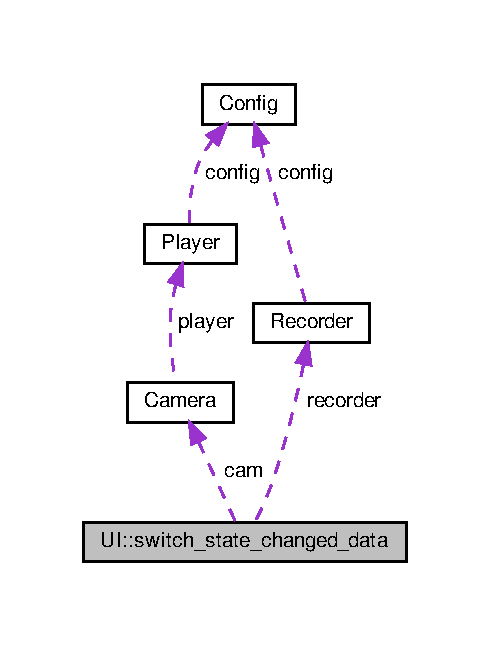
\includegraphics[width=235pt]{struct_u_i_1_1switch__state__changed__data__coll__graph}
\end{center}
\end{figure}
\subsection*{Открытые атрибуты}
\begin{DoxyCompactItemize}
\item 
\hyperlink{struct_camera}{Camera} $\ast$ \hyperlink{struct_u_i_1_1switch__state__changed__data_a40244e7ca16845eb02f4f7315ae98a89}{cam}
\item 
\hyperlink{class_recorder}{Recorder} $\ast$ \hyperlink{struct_u_i_1_1switch__state__changed__data_a9d4666f9a5533060e0a1ce07d74a240f}{recorder}
\end{DoxyCompactItemize}


\subsection{Данные класса}
\mbox{\Hypertarget{struct_u_i_1_1switch__state__changed__data_a40244e7ca16845eb02f4f7315ae98a89}\label{struct_u_i_1_1switch__state__changed__data_a40244e7ca16845eb02f4f7315ae98a89}} 
\index{U\+I\+::switch\+\_\+state\+\_\+changed\+\_\+data@{U\+I\+::switch\+\_\+state\+\_\+changed\+\_\+data}!cam@{cam}}
\index{cam@{cam}!U\+I\+::switch\+\_\+state\+\_\+changed\+\_\+data@{U\+I\+::switch\+\_\+state\+\_\+changed\+\_\+data}}
\subsubsection{\texorpdfstring{cam}{cam}}
{\footnotesize\ttfamily \hyperlink{struct_camera}{Camera}$\ast$ U\+I\+::switch\+\_\+state\+\_\+changed\+\_\+data\+::cam}

\mbox{\Hypertarget{struct_u_i_1_1switch__state__changed__data_a9d4666f9a5533060e0a1ce07d74a240f}\label{struct_u_i_1_1switch__state__changed__data_a9d4666f9a5533060e0a1ce07d74a240f}} 
\index{U\+I\+::switch\+\_\+state\+\_\+changed\+\_\+data@{U\+I\+::switch\+\_\+state\+\_\+changed\+\_\+data}!recorder@{recorder}}
\index{recorder@{recorder}!U\+I\+::switch\+\_\+state\+\_\+changed\+\_\+data@{U\+I\+::switch\+\_\+state\+\_\+changed\+\_\+data}}
\subsubsection{\texorpdfstring{recorder}{recorder}}
{\footnotesize\ttfamily \hyperlink{class_recorder}{Recorder}$\ast$ U\+I\+::switch\+\_\+state\+\_\+changed\+\_\+data\+::recorder}



Объявления и описания членов структуры находятся в файле\+:\begin{DoxyCompactItemize}
\item 
/home/jetson/controlroom/\+Studio/\+Recorder/include/\hyperlink{_recorder_2include_2ui_8h}{ui.\+h}\end{DoxyCompactItemize}

\hypertarget{class_u_i}{}\section{Класс UI}
\label{class_u_i}\index{UI@{UI}}


The \hyperlink{class_u_i}{UI} class.  




{\ttfamily \#include $<$ui.\+h$>$}



Граф связей класса UI\+:\nopagebreak
\begin{figure}[H]
\begin{center}
\leavevmode
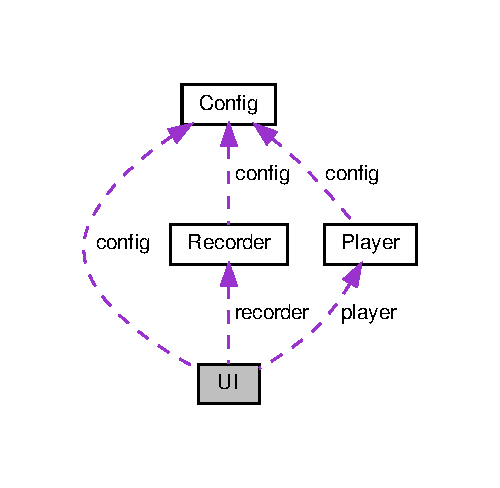
\includegraphics[width=240pt]{class_u_i__coll__graph}
\end{center}
\end{figure}
\subsection*{Классы}
\begin{DoxyCompactItemize}
\item 
struct \hyperlink{struct_u_i_1_1display__player__data}{display\+\_\+player\+\_\+data}
\item 
struct \hyperlink{struct_u_i_1_1gdrive__status__data}{gdrive\+\_\+status\+\_\+data}
\item 
struct \hyperlink{struct_u_i_1_1switch__state__changed__data}{switch\+\_\+state\+\_\+changed\+\_\+data}
\end{DoxyCompactItemize}
\subsection*{Открытые члены}
\begin{DoxyCompactItemize}
\item 
\hyperlink{class_u_i_a2b49119b809785f66dd97ce769ab1753}{UI} (\hyperlink{class_config}{Config} $\ast$\hyperlink{class_u_i_a6966022e569960221b61ea4f0111a484}{config})
\item 
\hyperlink{class_u_i_a1b23d0c64c7cbb3d143d90ec532a7ccd}{$\sim$\+UI} ()
\item 
\hyperlink{class_u_i_a2b49119b809785f66dd97ce769ab1753}{UI} (\hyperlink{class_config}{Config} $\ast$\hyperlink{class_u_i_a6966022e569960221b61ea4f0111a484}{config})
\item 
\hyperlink{class_u_i_a1b23d0c64c7cbb3d143d90ec532a7ccd}{$\sim$\+UI} ()
\item 
void \hyperlink{class_u_i_ad860928c87b2a7f4e18b3f6e15774dd3}{display\+Recording\+Status} (string cam\+\_\+id, bool status)
\end{DoxyCompactItemize}
\subsection*{Открытые атрибуты}
\begin{DoxyCompactItemize}
\item 
\hyperlink{class_config}{Config} $\ast$ \hyperlink{class_u_i_a6966022e569960221b61ea4f0111a484}{config}
\item 
string \hyperlink{class_u_i_a519609c35edd6f678d5d78fe88fac888}{playing\+Cam\+Name} = \char`\"{}\char`\"{}
\item 
\hyperlink{class_recorder}{Recorder} $\ast$ \hyperlink{class_u_i_aa857564b96618cd520b18b9c0ef95f00}{recorder}
\item 
vector$<$ Gtk\+Widget $\ast$ $>$ \hyperlink{class_u_i_a6e64500f18e96ae92dc4f584f37dfc4f}{switch\+GridV}
\end{DoxyCompactItemize}
\subsection*{Закрытые члены}
\begin{DoxyCompactItemize}
\item 
int \hyperlink{class_u_i_a2405c93cf8c14f22ebc20de45116e52b}{init\+Styles} ()
\item 
Gtk\+Widget $\ast$ \hyperlink{class_u_i_ad6b4d1f070f96f4a8cd7919595b2f9a7}{window\+Init} (Gtk\+Builder $\ast$$\ast$builder, string glade\+File, string window\+Name)
\item 
void \hyperlink{class_u_i_ac1d0ed7af2a3272527c544110fc37890}{init\+Menu\+Widgets} ()
\item 
void \hyperlink{class_u_i_abc8966cc08826d39716b86e0a160af24}{init\+Cam\+Widgets} (int room\+\_\+n, vector$<$ \hyperlink{struct_camera}{Camera} $>$ $\ast$cams)
\item 
void \hyperlink{class_u_i_ab66596071cbc18cb463b8a99266c7926}{init\+Room\+Tab} (int room\+\_\+n, string room\+\_\+name)
\item 
string \hyperlink{class_u_i_aa7991c3483e84d5ed9f64eeb333c9e44}{find\+IP} ()
\item 
int \hyperlink{class_u_i_a2405c93cf8c14f22ebc20de45116e52b}{init\+Styles} ()
\item 
Gtk\+Widget $\ast$ \hyperlink{class_u_i_ad65c4c017205871946a731f015d74f3c}{window\+Init} (Gtk\+Builder $\ast$$\ast$builder, string glade\+File, string window\+Name)
\item 
void \hyperlink{class_u_i_a85a2b2c92c5d2017f50886f7a184ddd1}{init\+Player\+Widgets} ()
\item 
void \hyperlink{class_u_i_ac1d0ed7af2a3272527c544110fc37890}{init\+Menu\+Widgets} ()
\item 
void \hyperlink{class_u_i_abc8966cc08826d39716b86e0a160af24}{init\+Cam\+Widgets} (int room\+\_\+n, vector$<$ \hyperlink{struct_camera}{Camera} $>$ $\ast$cams)
\item 
void \hyperlink{class_u_i_ab66596071cbc18cb463b8a99266c7926}{init\+Room\+Tab} (int room\+\_\+n, string room\+\_\+name)
\item 
string \hyperlink{class_u_i_aa7991c3483e84d5ed9f64eeb333c9e44}{find\+IP} ()
\end{DoxyCompactItemize}
\subsection*{Закрытые статические члены}
\begin{DoxyCompactItemize}
\item 
static int \hyperlink{class_u_i_a405d8c6cbfea57303917867587e7e523}{on\+\_\+show} (gpointer ui\+\_\+ptr)
\item 
static void \hyperlink{class_u_i_a4d6fc1c395de1396c3b4c17f60ce53f9}{page\+Switched} (Gtk\+Widget $\ast$widget, G\+Param\+Spec $\ast$property, vector$<$ \hyperlink{class_room}{Room} $\ast$$>$ $\ast$\hyperlink{class_u_i_ad5e9a6fd88afba6e3a647c75be137d13}{rooms})
\item 
static void \hyperlink{class_u_i_a48bcf14dfe5f38c4c531bf11f7e7217a}{display\+Player} (Gtk\+Widget $\ast$widget, gpointer data)
\item 
static gboolean \hyperlink{class_u_i_ae9d1de9359a28d1ec13f2824ec72420c}{key\+Press} (Gtk\+Widget $\ast$widget, Gdk\+Event\+Key $\ast$event, \hyperlink{class_u_i}{UI} $\ast$ui)
\item 
static gboolean \hyperlink{class_u_i_af5cf1161c6d50b6e1b1fbcfb6123e10f}{update\+G\+Drive\+Status} (gpointer user\+\_\+data)
\item 
static void \hyperlink{class_u_i_ae033d92357c8c8a175809bbee3e08b9b}{display\+Player} (Gtk\+Widget $\ast$widget, gpointer data)
\item 
static gboolean \hyperlink{class_u_i_ab9db8fde45ae6595a956feab77aaf2ca}{key\+Press} (Gtk\+Widget $\ast$widget, Gdk\+Event\+Key $\ast$event, \hyperlink{class_u_i}{UI} $\ast$ui)
\item 
static void \hyperlink{class_u_i_ad4a8a785914011267c9cba9ebe92cd23}{switch\+State\+Changed} (Gtk\+Widget $\ast$widget, gboolean state, gpointer user\+\_\+data)
\item 
static void \hyperlink{class_u_i_a2dfc8b3ab8c46094cabe6c8c332174cd}{edit\+Button\+Clicked} (Gtk\+Widget $\ast$widget, vector$<$ Gtk\+Widget $\ast$$>$ $\ast$\hyperlink{class_u_i_a6e64500f18e96ae92dc4f584f37dfc4f}{switch\+GridV})
\end{DoxyCompactItemize}
\subsection*{Закрытые данные}
\begin{DoxyCompactItemize}
\item 
vector$<$ \hyperlink{class_room}{Room} $\ast$ $>$ $\ast$ \hyperlink{class_u_i_ad5e9a6fd88afba6e3a647c75be137d13}{rooms}
\item 
map$<$ \hyperlink{struct_camera}{Camera} $\ast$, \hyperlink{class_player}{Player} $\ast$ $>$ \hyperlink{class_u_i_ac5805ed5874e6c85ad1e607a9080793e}{players}
\item 
Gtk\+Builder $\ast$ \hyperlink{class_u_i_a971badc03d122b8de17d37fec58157eb}{menu\+Builder}
\item 
Gtk\+Widget $\ast$ \hyperlink{class_u_i_a279e69dd8e9b22b5a2a9cfa117ac4446}{menu\+Window}
\item 
\hyperlink{class_player}{Player} $\ast$ \hyperlink{class_u_i_a201dd0c0bb94e697654b923090776a12}{player}
\item 
Gtk\+Builder $\ast$ \hyperlink{class_u_i_a460a7c95bf2db2595070f7c2a9009cc4}{player\+Builder}
\item 
Gtk\+Widget $\ast$ \hyperlink{class_u_i_acf7b7529c59af602e9d2642d881e9fdc}{player\+Window}
\item 
Gtk\+Widget $\ast$ \hyperlink{class_u_i_a809a7dd49c802ce7805bb6e1036b7ace}{player\+Widget}
\item 
Gtk\+Widget $\ast$ \hyperlink{class_u_i_ae6090309318f008e3497552119fc46b9}{player\+Label}
\item 
Gtk\+Widget $\ast$ \hyperlink{class_u_i_a3ebae98c80dca1700ddbfcb7b5b56ee8}{edit\+Button}
\end{DoxyCompactItemize}


\subsection{Подробное описание}
The \hyperlink{class_u_i}{UI} class. 

\subsection{Конструктор(ы)}
\mbox{\Hypertarget{class_u_i_a2b49119b809785f66dd97ce769ab1753}\label{class_u_i_a2b49119b809785f66dd97ce769ab1753}} 
\index{UI@{UI}!UI@{UI}}
\index{UI@{UI}!UI@{UI}}
\subsubsection{\texorpdfstring{U\+I()}{UI()}\hspace{0.1cm}{\footnotesize\ttfamily [1/2]}}
{\footnotesize\ttfamily U\+I\+::\+UI (\begin{DoxyParamCaption}\item[{\hyperlink{class_config}{Config} $\ast$}]{config }\end{DoxyParamCaption})}

Граф вызовов\+:\nopagebreak
\begin{figure}[H]
\begin{center}
\leavevmode
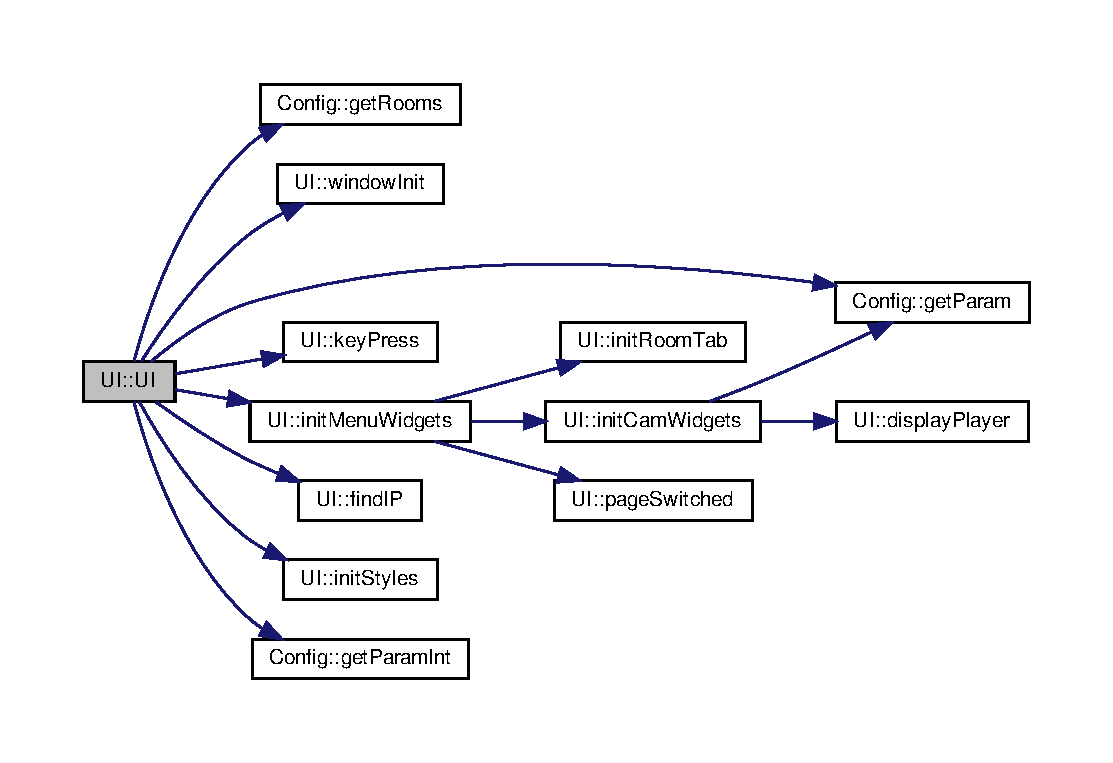
\includegraphics[width=350pt]{class_u_i_a2b49119b809785f66dd97ce769ab1753_cgraph}
\end{center}
\end{figure}
\mbox{\Hypertarget{class_u_i_a1b23d0c64c7cbb3d143d90ec532a7ccd}\label{class_u_i_a1b23d0c64c7cbb3d143d90ec532a7ccd}} 
\index{UI@{UI}!````~UI@{$\sim$\+UI}}
\index{````~UI@{$\sim$\+UI}!UI@{UI}}
\subsubsection{\texorpdfstring{$\sim$\+U\+I()}{~UI()}\hspace{0.1cm}{\footnotesize\ttfamily [1/2]}}
{\footnotesize\ttfamily U\+I\+::$\sim$\+UI (\begin{DoxyParamCaption}{ }\end{DoxyParamCaption})}

\mbox{\Hypertarget{class_u_i_a2b49119b809785f66dd97ce769ab1753}\label{class_u_i_a2b49119b809785f66dd97ce769ab1753}} 
\index{UI@{UI}!UI@{UI}}
\index{UI@{UI}!UI@{UI}}
\subsubsection{\texorpdfstring{U\+I()}{UI()}\hspace{0.1cm}{\footnotesize\ttfamily [2/2]}}
{\footnotesize\ttfamily U\+I\+::\+UI (\begin{DoxyParamCaption}\item[{\hyperlink{class_config}{Config} $\ast$}]{config }\end{DoxyParamCaption})}

\mbox{\Hypertarget{class_u_i_a1b23d0c64c7cbb3d143d90ec532a7ccd}\label{class_u_i_a1b23d0c64c7cbb3d143d90ec532a7ccd}} 
\index{UI@{UI}!````~UI@{$\sim$\+UI}}
\index{````~UI@{$\sim$\+UI}!UI@{UI}}
\subsubsection{\texorpdfstring{$\sim$\+U\+I()}{~UI()}\hspace{0.1cm}{\footnotesize\ttfamily [2/2]}}
{\footnotesize\ttfamily U\+I\+::$\sim$\+UI (\begin{DoxyParamCaption}{ }\end{DoxyParamCaption})}



\subsection{Методы}
\mbox{\Hypertarget{class_u_i_a48bcf14dfe5f38c4c531bf11f7e7217a}\label{class_u_i_a48bcf14dfe5f38c4c531bf11f7e7217a}} 
\index{UI@{UI}!display\+Player@{display\+Player}}
\index{display\+Player@{display\+Player}!UI@{UI}}
\subsubsection{\texorpdfstring{display\+Player()}{displayPlayer()}\hspace{0.1cm}{\footnotesize\ttfamily [1/2]}}
{\footnotesize\ttfamily void U\+I\+::display\+Player (\begin{DoxyParamCaption}\item[{Gtk\+Widget $\ast$}]{widget,  }\item[{gpointer}]{data }\end{DoxyParamCaption})\hspace{0.3cm}{\ttfamily [static]}, {\ttfamily [private]}}

\mbox{\Hypertarget{class_u_i_ae033d92357c8c8a175809bbee3e08b9b}\label{class_u_i_ae033d92357c8c8a175809bbee3e08b9b}} 
\index{UI@{UI}!display\+Player@{display\+Player}}
\index{display\+Player@{display\+Player}!UI@{UI}}
\subsubsection{\texorpdfstring{display\+Player()}{displayPlayer()}\hspace{0.1cm}{\footnotesize\ttfamily [2/2]}}
{\footnotesize\ttfamily static void U\+I\+::display\+Player (\begin{DoxyParamCaption}\item[{Gtk\+Widget $\ast$}]{widget,  }\item[{gpointer}]{data }\end{DoxyParamCaption})\hspace{0.3cm}{\ttfamily [static]}, {\ttfamily [private]}}

\mbox{\Hypertarget{class_u_i_ad860928c87b2a7f4e18b3f6e15774dd3}\label{class_u_i_ad860928c87b2a7f4e18b3f6e15774dd3}} 
\index{UI@{UI}!display\+Recording\+Status@{display\+Recording\+Status}}
\index{display\+Recording\+Status@{display\+Recording\+Status}!UI@{UI}}
\subsubsection{\texorpdfstring{display\+Recording\+Status()}{displayRecordingStatus()}}
{\footnotesize\ttfamily void U\+I\+::display\+Recording\+Status (\begin{DoxyParamCaption}\item[{string}]{cam\+\_\+id,  }\item[{bool}]{status }\end{DoxyParamCaption})}

\mbox{\Hypertarget{class_u_i_a2dfc8b3ab8c46094cabe6c8c332174cd}\label{class_u_i_a2dfc8b3ab8c46094cabe6c8c332174cd}} 
\index{UI@{UI}!edit\+Button\+Clicked@{edit\+Button\+Clicked}}
\index{edit\+Button\+Clicked@{edit\+Button\+Clicked}!UI@{UI}}
\subsubsection{\texorpdfstring{edit\+Button\+Clicked()}{editButtonClicked()}}
{\footnotesize\ttfamily void U\+I\+::edit\+Button\+Clicked (\begin{DoxyParamCaption}\item[{Gtk\+Widget $\ast$}]{widget,  }\item[{vector$<$ Gtk\+Widget $\ast$$>$ $\ast$}]{switch\+GridV }\end{DoxyParamCaption})\hspace{0.3cm}{\ttfamily [static]}, {\ttfamily [private]}}

Граф вызовов\+:\nopagebreak
\begin{figure}[H]
\begin{center}
\leavevmode
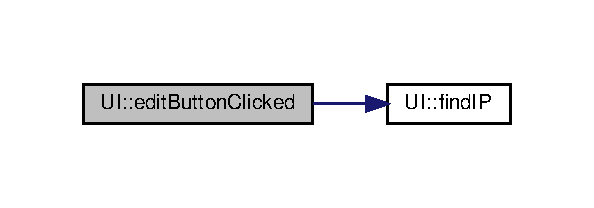
\includegraphics[width=285pt]{class_u_i_a2dfc8b3ab8c46094cabe6c8c332174cd_cgraph}
\end{center}
\end{figure}
\mbox{\Hypertarget{class_u_i_aa7991c3483e84d5ed9f64eeb333c9e44}\label{class_u_i_aa7991c3483e84d5ed9f64eeb333c9e44}} 
\index{UI@{UI}!find\+IP@{find\+IP}}
\index{find\+IP@{find\+IP}!UI@{UI}}
\subsubsection{\texorpdfstring{find\+I\+P()}{findIP()}\hspace{0.1cm}{\footnotesize\ttfamily [1/2]}}
{\footnotesize\ttfamily string U\+I\+::find\+IP (\begin{DoxyParamCaption}{ }\end{DoxyParamCaption})\hspace{0.3cm}{\ttfamily [private]}}

\mbox{\Hypertarget{class_u_i_aa7991c3483e84d5ed9f64eeb333c9e44}\label{class_u_i_aa7991c3483e84d5ed9f64eeb333c9e44}} 
\index{UI@{UI}!find\+IP@{find\+IP}}
\index{find\+IP@{find\+IP}!UI@{UI}}
\subsubsection{\texorpdfstring{find\+I\+P()}{findIP()}\hspace{0.1cm}{\footnotesize\ttfamily [2/2]}}
{\footnotesize\ttfamily string U\+I\+::find\+IP (\begin{DoxyParamCaption}{ }\end{DoxyParamCaption})\hspace{0.3cm}{\ttfamily [private]}}

\mbox{\Hypertarget{class_u_i_abc8966cc08826d39716b86e0a160af24}\label{class_u_i_abc8966cc08826d39716b86e0a160af24}} 
\index{UI@{UI}!init\+Cam\+Widgets@{init\+Cam\+Widgets}}
\index{init\+Cam\+Widgets@{init\+Cam\+Widgets}!UI@{UI}}
\subsubsection{\texorpdfstring{init\+Cam\+Widgets()}{initCamWidgets()}\hspace{0.1cm}{\footnotesize\ttfamily [1/2]}}
{\footnotesize\ttfamily void U\+I\+::init\+Cam\+Widgets (\begin{DoxyParamCaption}\item[{int}]{room\+\_\+n,  }\item[{vector$<$ \hyperlink{struct_camera}{Camera} $>$ $\ast$}]{cams }\end{DoxyParamCaption})\hspace{0.3cm}{\ttfamily [private]}}

Граф вызовов\+:\nopagebreak
\begin{figure}[H]
\begin{center}
\leavevmode
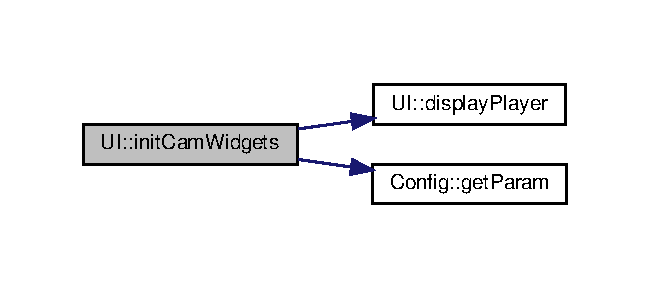
\includegraphics[width=312pt]{class_u_i_abc8966cc08826d39716b86e0a160af24_cgraph}
\end{center}
\end{figure}
\mbox{\Hypertarget{class_u_i_abc8966cc08826d39716b86e0a160af24}\label{class_u_i_abc8966cc08826d39716b86e0a160af24}} 
\index{UI@{UI}!init\+Cam\+Widgets@{init\+Cam\+Widgets}}
\index{init\+Cam\+Widgets@{init\+Cam\+Widgets}!UI@{UI}}
\subsubsection{\texorpdfstring{init\+Cam\+Widgets()}{initCamWidgets()}\hspace{0.1cm}{\footnotesize\ttfamily [2/2]}}
{\footnotesize\ttfamily void U\+I\+::init\+Cam\+Widgets (\begin{DoxyParamCaption}\item[{int}]{room\+\_\+n,  }\item[{vector$<$ \hyperlink{struct_camera}{Camera} $>$ $\ast$}]{cams }\end{DoxyParamCaption})\hspace{0.3cm}{\ttfamily [private]}}

\mbox{\Hypertarget{class_u_i_ac1d0ed7af2a3272527c544110fc37890}\label{class_u_i_ac1d0ed7af2a3272527c544110fc37890}} 
\index{UI@{UI}!init\+Menu\+Widgets@{init\+Menu\+Widgets}}
\index{init\+Menu\+Widgets@{init\+Menu\+Widgets}!UI@{UI}}
\subsubsection{\texorpdfstring{init\+Menu\+Widgets()}{initMenuWidgets()}\hspace{0.1cm}{\footnotesize\ttfamily [1/2]}}
{\footnotesize\ttfamily void U\+I\+::init\+Menu\+Widgets (\begin{DoxyParamCaption}{ }\end{DoxyParamCaption})\hspace{0.3cm}{\ttfamily [private]}}

Граф вызовов\+:\nopagebreak
\begin{figure}[H]
\begin{center}
\leavevmode
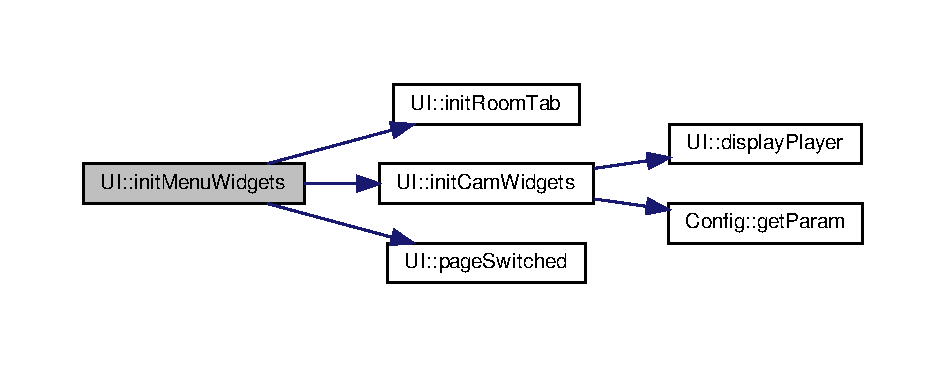
\includegraphics[width=350pt]{class_u_i_ac1d0ed7af2a3272527c544110fc37890_cgraph}
\end{center}
\end{figure}
\mbox{\Hypertarget{class_u_i_ac1d0ed7af2a3272527c544110fc37890}\label{class_u_i_ac1d0ed7af2a3272527c544110fc37890}} 
\index{UI@{UI}!init\+Menu\+Widgets@{init\+Menu\+Widgets}}
\index{init\+Menu\+Widgets@{init\+Menu\+Widgets}!UI@{UI}}
\subsubsection{\texorpdfstring{init\+Menu\+Widgets()}{initMenuWidgets()}\hspace{0.1cm}{\footnotesize\ttfamily [2/2]}}
{\footnotesize\ttfamily void U\+I\+::init\+Menu\+Widgets (\begin{DoxyParamCaption}{ }\end{DoxyParamCaption})\hspace{0.3cm}{\ttfamily [private]}}

\mbox{\Hypertarget{class_u_i_a85a2b2c92c5d2017f50886f7a184ddd1}\label{class_u_i_a85a2b2c92c5d2017f50886f7a184ddd1}} 
\index{UI@{UI}!init\+Player\+Widgets@{init\+Player\+Widgets}}
\index{init\+Player\+Widgets@{init\+Player\+Widgets}!UI@{UI}}
\subsubsection{\texorpdfstring{init\+Player\+Widgets()}{initPlayerWidgets()}}
{\footnotesize\ttfamily void U\+I\+::init\+Player\+Widgets (\begin{DoxyParamCaption}{ }\end{DoxyParamCaption})\hspace{0.3cm}{\ttfamily [private]}}

Граф вызовов\+:\nopagebreak
\begin{figure}[H]
\begin{center}
\leavevmode
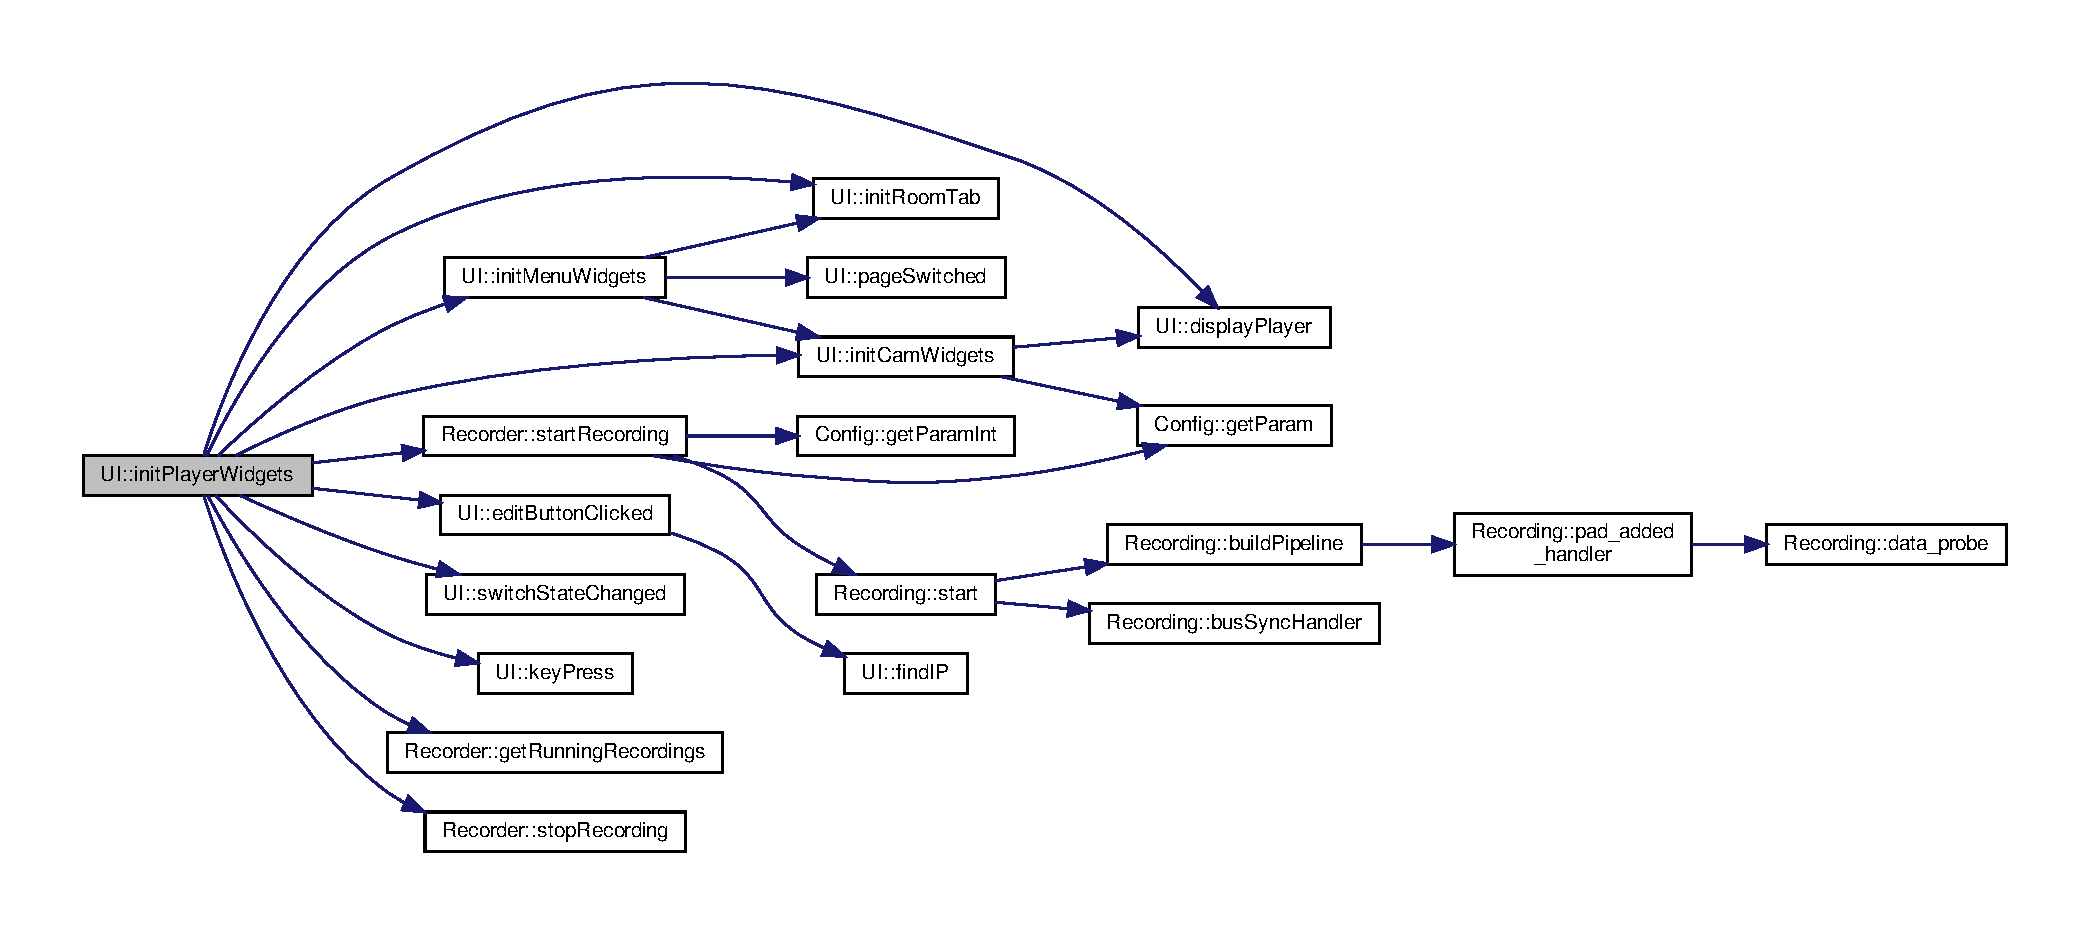
\includegraphics[width=350pt]{class_u_i_a85a2b2c92c5d2017f50886f7a184ddd1_cgraph}
\end{center}
\end{figure}
\mbox{\Hypertarget{class_u_i_ab66596071cbc18cb463b8a99266c7926}\label{class_u_i_ab66596071cbc18cb463b8a99266c7926}} 
\index{UI@{UI}!init\+Room\+Tab@{init\+Room\+Tab}}
\index{init\+Room\+Tab@{init\+Room\+Tab}!UI@{UI}}
\subsubsection{\texorpdfstring{init\+Room\+Tab()}{initRoomTab()}\hspace{0.1cm}{\footnotesize\ttfamily [1/2]}}
{\footnotesize\ttfamily void U\+I\+::init\+Room\+Tab (\begin{DoxyParamCaption}\item[{int}]{room\+\_\+n,  }\item[{string}]{room\+\_\+name }\end{DoxyParamCaption})\hspace{0.3cm}{\ttfamily [private]}}

\mbox{\Hypertarget{class_u_i_ab66596071cbc18cb463b8a99266c7926}\label{class_u_i_ab66596071cbc18cb463b8a99266c7926}} 
\index{UI@{UI}!init\+Room\+Tab@{init\+Room\+Tab}}
\index{init\+Room\+Tab@{init\+Room\+Tab}!UI@{UI}}
\subsubsection{\texorpdfstring{init\+Room\+Tab()}{initRoomTab()}\hspace{0.1cm}{\footnotesize\ttfamily [2/2]}}
{\footnotesize\ttfamily void U\+I\+::init\+Room\+Tab (\begin{DoxyParamCaption}\item[{int}]{room\+\_\+n,  }\item[{string}]{room\+\_\+name }\end{DoxyParamCaption})\hspace{0.3cm}{\ttfamily [private]}}

\mbox{\Hypertarget{class_u_i_a2405c93cf8c14f22ebc20de45116e52b}\label{class_u_i_a2405c93cf8c14f22ebc20de45116e52b}} 
\index{UI@{UI}!init\+Styles@{init\+Styles}}
\index{init\+Styles@{init\+Styles}!UI@{UI}}
\subsubsection{\texorpdfstring{init\+Styles()}{initStyles()}\hspace{0.1cm}{\footnotesize\ttfamily [1/2]}}
{\footnotesize\ttfamily int U\+I\+::init\+Styles (\begin{DoxyParamCaption}{ }\end{DoxyParamCaption})\hspace{0.3cm}{\ttfamily [private]}}

\mbox{\Hypertarget{class_u_i_a2405c93cf8c14f22ebc20de45116e52b}\label{class_u_i_a2405c93cf8c14f22ebc20de45116e52b}} 
\index{UI@{UI}!init\+Styles@{init\+Styles}}
\index{init\+Styles@{init\+Styles}!UI@{UI}}
\subsubsection{\texorpdfstring{init\+Styles()}{initStyles()}\hspace{0.1cm}{\footnotesize\ttfamily [2/2]}}
{\footnotesize\ttfamily int U\+I\+::init\+Styles (\begin{DoxyParamCaption}{ }\end{DoxyParamCaption})\hspace{0.3cm}{\ttfamily [private]}}

\mbox{\Hypertarget{class_u_i_ae9d1de9359a28d1ec13f2824ec72420c}\label{class_u_i_ae9d1de9359a28d1ec13f2824ec72420c}} 
\index{UI@{UI}!key\+Press@{key\+Press}}
\index{key\+Press@{key\+Press}!UI@{UI}}
\subsubsection{\texorpdfstring{key\+Press()}{keyPress()}\hspace{0.1cm}{\footnotesize\ttfamily [1/2]}}
{\footnotesize\ttfamily gboolean U\+I\+::key\+Press (\begin{DoxyParamCaption}\item[{Gtk\+Widget $\ast$}]{widget,  }\item[{Gdk\+Event\+Key $\ast$}]{event,  }\item[{\hyperlink{class_u_i}{UI} $\ast$}]{ui }\end{DoxyParamCaption})\hspace{0.3cm}{\ttfamily [static]}, {\ttfamily [private]}}

\mbox{\Hypertarget{class_u_i_ab9db8fde45ae6595a956feab77aaf2ca}\label{class_u_i_ab9db8fde45ae6595a956feab77aaf2ca}} 
\index{UI@{UI}!key\+Press@{key\+Press}}
\index{key\+Press@{key\+Press}!UI@{UI}}
\subsubsection{\texorpdfstring{key\+Press()}{keyPress()}\hspace{0.1cm}{\footnotesize\ttfamily [2/2]}}
{\footnotesize\ttfamily static gboolean U\+I\+::key\+Press (\begin{DoxyParamCaption}\item[{Gtk\+Widget $\ast$}]{widget,  }\item[{Gdk\+Event\+Key $\ast$}]{event,  }\item[{\hyperlink{class_u_i}{UI} $\ast$}]{ui }\end{DoxyParamCaption})\hspace{0.3cm}{\ttfamily [static]}, {\ttfamily [private]}}

\mbox{\Hypertarget{class_u_i_a405d8c6cbfea57303917867587e7e523}\label{class_u_i_a405d8c6cbfea57303917867587e7e523}} 
\index{UI@{UI}!on\+\_\+show@{on\+\_\+show}}
\index{on\+\_\+show@{on\+\_\+show}!UI@{UI}}
\subsubsection{\texorpdfstring{on\+\_\+show()}{on\_show()}}
{\footnotesize\ttfamily int U\+I\+::on\+\_\+show (\begin{DoxyParamCaption}\item[{gpointer}]{ui\+\_\+ptr }\end{DoxyParamCaption})\hspace{0.3cm}{\ttfamily [static]}, {\ttfamily [private]}}

Граф вызовов\+:\nopagebreak
\begin{figure}[H]
\begin{center}
\leavevmode
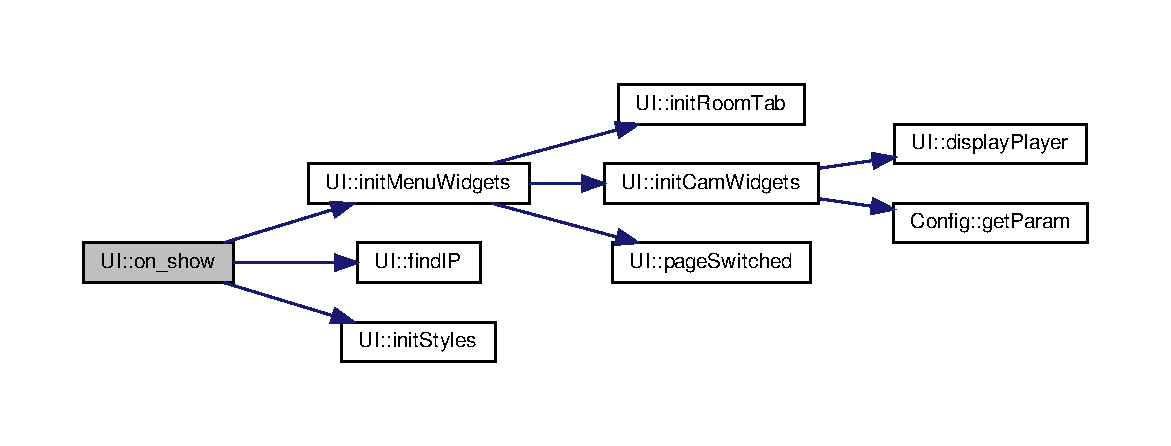
\includegraphics[width=350pt]{class_u_i_a405d8c6cbfea57303917867587e7e523_cgraph}
\end{center}
\end{figure}
\mbox{\Hypertarget{class_u_i_a4d6fc1c395de1396c3b4c17f60ce53f9}\label{class_u_i_a4d6fc1c395de1396c3b4c17f60ce53f9}} 
\index{UI@{UI}!page\+Switched@{page\+Switched}}
\index{page\+Switched@{page\+Switched}!UI@{UI}}
\subsubsection{\texorpdfstring{page\+Switched()}{pageSwitched()}}
{\footnotesize\ttfamily void U\+I\+::page\+Switched (\begin{DoxyParamCaption}\item[{Gtk\+Widget $\ast$}]{widget,  }\item[{G\+Param\+Spec $\ast$}]{property,  }\item[{vector$<$ \hyperlink{class_room}{Room} $\ast$$>$ $\ast$}]{rooms }\end{DoxyParamCaption})\hspace{0.3cm}{\ttfamily [static]}, {\ttfamily [private]}}

\mbox{\Hypertarget{class_u_i_ad4a8a785914011267c9cba9ebe92cd23}\label{class_u_i_ad4a8a785914011267c9cba9ebe92cd23}} 
\index{UI@{UI}!switch\+State\+Changed@{switch\+State\+Changed}}
\index{switch\+State\+Changed@{switch\+State\+Changed}!UI@{UI}}
\subsubsection{\texorpdfstring{switch\+State\+Changed()}{switchStateChanged()}}
{\footnotesize\ttfamily void U\+I\+::switch\+State\+Changed (\begin{DoxyParamCaption}\item[{Gtk\+Widget $\ast$}]{widget,  }\item[{gboolean}]{state,  }\item[{gpointer}]{user\+\_\+data }\end{DoxyParamCaption})\hspace{0.3cm}{\ttfamily [static]}, {\ttfamily [private]}}

\mbox{\Hypertarget{class_u_i_af5cf1161c6d50b6e1b1fbcfb6123e10f}\label{class_u_i_af5cf1161c6d50b6e1b1fbcfb6123e10f}} 
\index{UI@{UI}!update\+G\+Drive\+Status@{update\+G\+Drive\+Status}}
\index{update\+G\+Drive\+Status@{update\+G\+Drive\+Status}!UI@{UI}}
\subsubsection{\texorpdfstring{update\+G\+Drive\+Status()}{updateGDriveStatus()}}
{\footnotesize\ttfamily gboolean U\+I\+::update\+G\+Drive\+Status (\begin{DoxyParamCaption}\item[{gpointer}]{user\+\_\+data }\end{DoxyParamCaption})\hspace{0.3cm}{\ttfamily [static]}, {\ttfamily [private]}}

Граф вызовов\+:\nopagebreak
\begin{figure}[H]
\begin{center}
\leavevmode
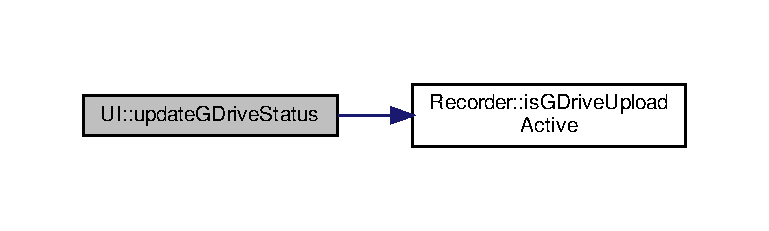
\includegraphics[width=350pt]{class_u_i_af5cf1161c6d50b6e1b1fbcfb6123e10f_cgraph}
\end{center}
\end{figure}
\mbox{\Hypertarget{class_u_i_ad6b4d1f070f96f4a8cd7919595b2f9a7}\label{class_u_i_ad6b4d1f070f96f4a8cd7919595b2f9a7}} 
\index{UI@{UI}!window\+Init@{window\+Init}}
\index{window\+Init@{window\+Init}!UI@{UI}}
\subsubsection{\texorpdfstring{window\+Init()}{windowInit()}\hspace{0.1cm}{\footnotesize\ttfamily [1/2]}}
{\footnotesize\ttfamily Gtk\+Widget $\ast$ U\+I\+::window\+Init (\begin{DoxyParamCaption}\item[{Gtk\+Builder $\ast$$\ast$}]{builder,  }\item[{string}]{glade\+File,  }\item[{string}]{window\+Name }\end{DoxyParamCaption})\hspace{0.3cm}{\ttfamily [private]}}

\mbox{\Hypertarget{class_u_i_ad65c4c017205871946a731f015d74f3c}\label{class_u_i_ad65c4c017205871946a731f015d74f3c}} 
\index{UI@{UI}!window\+Init@{window\+Init}}
\index{window\+Init@{window\+Init}!UI@{UI}}
\subsubsection{\texorpdfstring{window\+Init()}{windowInit()}\hspace{0.1cm}{\footnotesize\ttfamily [2/2]}}
{\footnotesize\ttfamily Gtk\+Widget$\ast$ U\+I\+::window\+Init (\begin{DoxyParamCaption}\item[{Gtk\+Builder $\ast$$\ast$}]{builder,  }\item[{string}]{glade\+File,  }\item[{string}]{window\+Name }\end{DoxyParamCaption})\hspace{0.3cm}{\ttfamily [private]}}



\subsection{Данные класса}
\mbox{\Hypertarget{class_u_i_a6966022e569960221b61ea4f0111a484}\label{class_u_i_a6966022e569960221b61ea4f0111a484}} 
\index{UI@{UI}!config@{config}}
\index{config@{config}!UI@{UI}}
\subsubsection{\texorpdfstring{config}{config}}
{\footnotesize\ttfamily \hyperlink{class_config}{Config} $\ast$ U\+I\+::config}

\mbox{\Hypertarget{class_u_i_a3ebae98c80dca1700ddbfcb7b5b56ee8}\label{class_u_i_a3ebae98c80dca1700ddbfcb7b5b56ee8}} 
\index{UI@{UI}!edit\+Button@{edit\+Button}}
\index{edit\+Button@{edit\+Button}!UI@{UI}}
\subsubsection{\texorpdfstring{edit\+Button}{editButton}}
{\footnotesize\ttfamily Gtk\+Widget$\ast$ U\+I\+::edit\+Button\hspace{0.3cm}{\ttfamily [private]}}

\mbox{\Hypertarget{class_u_i_a971badc03d122b8de17d37fec58157eb}\label{class_u_i_a971badc03d122b8de17d37fec58157eb}} 
\index{UI@{UI}!menu\+Builder@{menu\+Builder}}
\index{menu\+Builder@{menu\+Builder}!UI@{UI}}
\subsubsection{\texorpdfstring{menu\+Builder}{menuBuilder}}
{\footnotesize\ttfamily Gtk\+Builder $\ast$ U\+I\+::menu\+Builder\hspace{0.3cm}{\ttfamily [private]}}

\mbox{\Hypertarget{class_u_i_a279e69dd8e9b22b5a2a9cfa117ac4446}\label{class_u_i_a279e69dd8e9b22b5a2a9cfa117ac4446}} 
\index{UI@{UI}!menu\+Window@{menu\+Window}}
\index{menu\+Window@{menu\+Window}!UI@{UI}}
\subsubsection{\texorpdfstring{menu\+Window}{menuWindow}}
{\footnotesize\ttfamily Gtk\+Widget $\ast$ U\+I\+::menu\+Window\hspace{0.3cm}{\ttfamily [private]}}

\mbox{\Hypertarget{class_u_i_a201dd0c0bb94e697654b923090776a12}\label{class_u_i_a201dd0c0bb94e697654b923090776a12}} 
\index{UI@{UI}!player@{player}}
\index{player@{player}!UI@{UI}}
\subsubsection{\texorpdfstring{player}{player}}
{\footnotesize\ttfamily \hyperlink{class_player}{Player}$\ast$ U\+I\+::player\hspace{0.3cm}{\ttfamily [private]}}

\mbox{\Hypertarget{class_u_i_a460a7c95bf2db2595070f7c2a9009cc4}\label{class_u_i_a460a7c95bf2db2595070f7c2a9009cc4}} 
\index{UI@{UI}!player\+Builder@{player\+Builder}}
\index{player\+Builder@{player\+Builder}!UI@{UI}}
\subsubsection{\texorpdfstring{player\+Builder}{playerBuilder}}
{\footnotesize\ttfamily Gtk\+Builder $\ast$ U\+I\+::player\+Builder\hspace{0.3cm}{\ttfamily [private]}}

\mbox{\Hypertarget{class_u_i_ae6090309318f008e3497552119fc46b9}\label{class_u_i_ae6090309318f008e3497552119fc46b9}} 
\index{UI@{UI}!player\+Label@{player\+Label}}
\index{player\+Label@{player\+Label}!UI@{UI}}
\subsubsection{\texorpdfstring{player\+Label}{playerLabel}}
{\footnotesize\ttfamily Gtk\+Widget $\ast$ U\+I\+::player\+Label\hspace{0.3cm}{\ttfamily [private]}}

\mbox{\Hypertarget{class_u_i_ac5805ed5874e6c85ad1e607a9080793e}\label{class_u_i_ac5805ed5874e6c85ad1e607a9080793e}} 
\index{UI@{UI}!players@{players}}
\index{players@{players}!UI@{UI}}
\subsubsection{\texorpdfstring{players}{players}}
{\footnotesize\ttfamily map$<$\hyperlink{struct_camera}{Camera}$\ast$, \hyperlink{class_player}{Player}$\ast$$>$ U\+I\+::players\hspace{0.3cm}{\ttfamily [private]}}

\mbox{\Hypertarget{class_u_i_a809a7dd49c802ce7805bb6e1036b7ace}\label{class_u_i_a809a7dd49c802ce7805bb6e1036b7ace}} 
\index{UI@{UI}!player\+Widget@{player\+Widget}}
\index{player\+Widget@{player\+Widget}!UI@{UI}}
\subsubsection{\texorpdfstring{player\+Widget}{playerWidget}}
{\footnotesize\ttfamily Gtk\+Widget$\ast$ U\+I\+::player\+Widget\hspace{0.3cm}{\ttfamily [private]}}

\mbox{\Hypertarget{class_u_i_acf7b7529c59af602e9d2642d881e9fdc}\label{class_u_i_acf7b7529c59af602e9d2642d881e9fdc}} 
\index{UI@{UI}!player\+Window@{player\+Window}}
\index{player\+Window@{player\+Window}!UI@{UI}}
\subsubsection{\texorpdfstring{player\+Window}{playerWindow}}
{\footnotesize\ttfamily Gtk\+Widget $\ast$ U\+I\+::player\+Window\hspace{0.3cm}{\ttfamily [private]}}

\mbox{\Hypertarget{class_u_i_a519609c35edd6f678d5d78fe88fac888}\label{class_u_i_a519609c35edd6f678d5d78fe88fac888}} 
\index{UI@{UI}!playing\+Cam\+Name@{playing\+Cam\+Name}}
\index{playing\+Cam\+Name@{playing\+Cam\+Name}!UI@{UI}}
\subsubsection{\texorpdfstring{playing\+Cam\+Name}{playingCamName}}
{\footnotesize\ttfamily string U\+I\+::playing\+Cam\+Name = \char`\"{}\char`\"{}}

\mbox{\Hypertarget{class_u_i_aa857564b96618cd520b18b9c0ef95f00}\label{class_u_i_aa857564b96618cd520b18b9c0ef95f00}} 
\index{UI@{UI}!recorder@{recorder}}
\index{recorder@{recorder}!UI@{UI}}
\subsubsection{\texorpdfstring{recorder}{recorder}}
{\footnotesize\ttfamily \hyperlink{class_recorder}{Recorder}$\ast$ U\+I\+::recorder}

\mbox{\Hypertarget{class_u_i_ad5e9a6fd88afba6e3a647c75be137d13}\label{class_u_i_ad5e9a6fd88afba6e3a647c75be137d13}} 
\index{UI@{UI}!rooms@{rooms}}
\index{rooms@{rooms}!UI@{UI}}
\subsubsection{\texorpdfstring{rooms}{rooms}}
{\footnotesize\ttfamily vector$<$ \hyperlink{class_room}{Room} $\ast$ $>$ $\ast$ U\+I\+::rooms\hspace{0.3cm}{\ttfamily [private]}}

\mbox{\Hypertarget{class_u_i_a6e64500f18e96ae92dc4f584f37dfc4f}\label{class_u_i_a6e64500f18e96ae92dc4f584f37dfc4f}} 
\index{UI@{UI}!switch\+GridV@{switch\+GridV}}
\index{switch\+GridV@{switch\+GridV}!UI@{UI}}
\subsubsection{\texorpdfstring{switch\+GridV}{switchGridV}}
{\footnotesize\ttfamily vector$<$Gtk\+Widget$\ast$$>$ U\+I\+::switch\+GridV}



Объявления и описания членов классов находятся в файлах\+:\begin{DoxyCompactItemize}
\item 
/home/jetson/controlroom/\+Studio/\+Operator/\+Grid/include/\hyperlink{_operator_2_grid_2include_2ui_8h}{ui.\+h}\item 
/home/jetson/controlroom/\+Studio/\+Operator/\+Grid/src/\hyperlink{_operator_2_grid_2src_2ui_8cpp}{ui.\+cpp}\end{DoxyCompactItemize}

\hypertarget{classnetwork__monitor_1_1_u_i_graph}{}\section{Класс network\+\_\+monitor.\+U\+I\+Graph}
\label{classnetwork__monitor_1_1_u_i_graph}\index{network\+\_\+monitor.\+U\+I\+Graph@{network\+\_\+monitor.\+U\+I\+Graph}}


Граф наследования\+:network\+\_\+monitor.\+U\+I\+Graph\+:\nopagebreak
\begin{figure}[H]
\begin{center}
\leavevmode
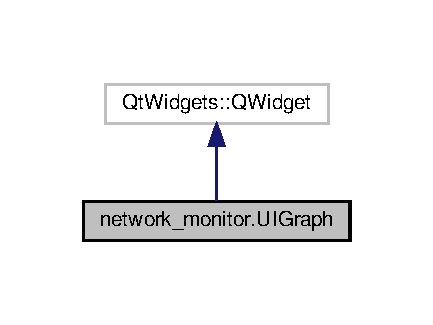
\includegraphics[width=208pt]{classnetwork__monitor_1_1_u_i_graph__inherit__graph}
\end{center}
\end{figure}


Граф связей класса network\+\_\+monitor.\+U\+I\+Graph\+:\nopagebreak
\begin{figure}[H]
\begin{center}
\leavevmode
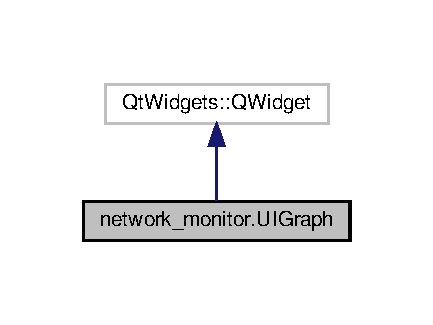
\includegraphics[width=208pt]{classnetwork__monitor_1_1_u_i_graph__coll__graph}
\end{center}
\end{figure}
\subsection*{Открытые члены}
\begin{DoxyCompactItemize}
\item 
def \hyperlink{classnetwork__monitor_1_1_u_i_graph_a6226e31f29149231ae294fdfa67a6fc7}{\+\_\+\+\_\+init\+\_\+\+\_\+} (self)
\end{DoxyCompactItemize}


\subsection{Конструктор(ы)}
\mbox{\Hypertarget{classnetwork__monitor_1_1_u_i_graph_a6226e31f29149231ae294fdfa67a6fc7}\label{classnetwork__monitor_1_1_u_i_graph_a6226e31f29149231ae294fdfa67a6fc7}} 
\index{network\+\_\+monitor\+::\+U\+I\+Graph@{network\+\_\+monitor\+::\+U\+I\+Graph}!\+\_\+\+\_\+init\+\_\+\+\_\+@{\+\_\+\+\_\+init\+\_\+\+\_\+}}
\index{\+\_\+\+\_\+init\+\_\+\+\_\+@{\+\_\+\+\_\+init\+\_\+\+\_\+}!network\+\_\+monitor\+::\+U\+I\+Graph@{network\+\_\+monitor\+::\+U\+I\+Graph}}
\subsubsection{\texorpdfstring{\+\_\+\+\_\+init\+\_\+\+\_\+()}{\_\_init\_\_()}}
{\footnotesize\ttfamily def network\+\_\+monitor.\+U\+I\+Graph.\+\_\+\+\_\+init\+\_\+\+\_\+ (\begin{DoxyParamCaption}\item[{}]{self }\end{DoxyParamCaption})}



Объявления и описания членов класса находятся в файле\+:\begin{DoxyCompactItemize}
\item 
/home/jetson/controlroom/\+Studio/\+Network/src/\hyperlink{network__monitor_8py}{network\+\_\+monitor.\+py}\end{DoxyCompactItemize}

\hypertarget{classnetwork__monitor_1_1_u_i_menu}{}\section{Класс network\+\_\+monitor.\+U\+I\+Menu}
\label{classnetwork__monitor_1_1_u_i_menu}\index{network\+\_\+monitor.\+U\+I\+Menu@{network\+\_\+monitor.\+U\+I\+Menu}}


Граф наследования\+:network\+\_\+monitor.\+U\+I\+Menu\+:\nopagebreak
\begin{figure}[H]
\begin{center}
\leavevmode
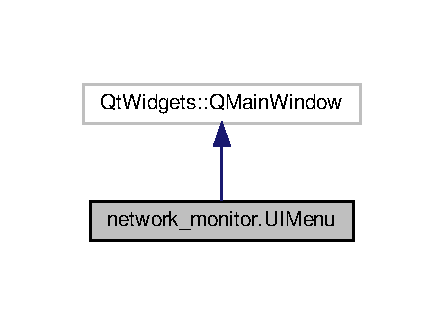
\includegraphics[width=213pt]{classnetwork__monitor_1_1_u_i_menu__inherit__graph}
\end{center}
\end{figure}


Граф связей класса network\+\_\+monitor.\+U\+I\+Menu\+:\nopagebreak
\begin{figure}[H]
\begin{center}
\leavevmode
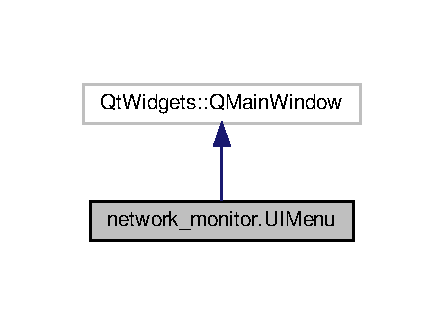
\includegraphics[width=213pt]{classnetwork__monitor_1_1_u_i_menu__coll__graph}
\end{center}
\end{figure}
\subsection*{Открытые члены}
\begin{DoxyCompactItemize}
\item 
def \hyperlink{classnetwork__monitor_1_1_u_i_menu_a2747f83c587a0d29338be7d190c7ab0c}{\+\_\+\+\_\+init\+\_\+\+\_\+} (self)
\end{DoxyCompactItemize}


\subsection{Конструктор(ы)}
\mbox{\Hypertarget{classnetwork__monitor_1_1_u_i_menu_a2747f83c587a0d29338be7d190c7ab0c}\label{classnetwork__monitor_1_1_u_i_menu_a2747f83c587a0d29338be7d190c7ab0c}} 
\index{network\+\_\+monitor\+::\+U\+I\+Menu@{network\+\_\+monitor\+::\+U\+I\+Menu}!\+\_\+\+\_\+init\+\_\+\+\_\+@{\+\_\+\+\_\+init\+\_\+\+\_\+}}
\index{\+\_\+\+\_\+init\+\_\+\+\_\+@{\+\_\+\+\_\+init\+\_\+\+\_\+}!network\+\_\+monitor\+::\+U\+I\+Menu@{network\+\_\+monitor\+::\+U\+I\+Menu}}
\subsubsection{\texorpdfstring{\+\_\+\+\_\+init\+\_\+\+\_\+()}{\_\_init\_\_()}}
{\footnotesize\ttfamily def network\+\_\+monitor.\+U\+I\+Menu.\+\_\+\+\_\+init\+\_\+\+\_\+ (\begin{DoxyParamCaption}\item[{}]{self }\end{DoxyParamCaption})}



Объявления и описания членов класса находятся в файле\+:\begin{DoxyCompactItemize}
\item 
/home/jetson/controlroom/\+Studio/\+Network/src/\hyperlink{network__monitor_8py}{network\+\_\+monitor.\+py}\end{DoxyCompactItemize}

\chapter{Файлы}
\hypertarget{groups_8dox}{}\section{Файл groups.\+dox}
\label{groups_8dox}\index{groups.\+dox@{groups.\+dox}}

\hypertarget{network__monitor_8py}{}\section{Файл /home/jetson/controlroom/\+Studio/\+Network/src/network\+\_\+monitor.py}
\label{network__monitor_8py}\index{/home/jetson/controlroom/\+Studio/\+Network/src/network\+\_\+monitor.\+py@{/home/jetson/controlroom/\+Studio/\+Network/src/network\+\_\+monitor.\+py}}
\subsection*{Классы}
\begin{DoxyCompactItemize}
\item 
class \hyperlink{classnetwork__monitor_1_1_u_i_menu}{network\+\_\+monitor.\+U\+I\+Menu}
\item 
class \hyperlink{classnetwork__monitor_1_1_u_i_graph}{network\+\_\+monitor.\+U\+I\+Graph}
\item 
class \hyperlink{classnetwork__monitor_1_1_pinger}{network\+\_\+monitor.\+Pinger}
\begin{DoxyCompactList}\small\item\em Пингует камеры \end{DoxyCompactList}\item 
class \hyperlink{classnetwork__monitor_1_1_grapher}{network\+\_\+monitor.\+Grapher}
\item 
class \hyperlink{classnetwork__monitor_1_1_camera}{network\+\_\+monitor.\+Camera}
\end{DoxyCompactItemize}
\subsection*{Пространства имен}
\begin{DoxyCompactItemize}
\item 
 \hyperlink{namespacenetwork__monitor}{network\+\_\+monitor}
\end{DoxyCompactItemize}
\subsection*{Функции}
\begin{DoxyCompactItemize}
\item 
def \hyperlink{namespacenetwork__monitor_aa615228bd6f33e03eb168421f8980368}{network\+\_\+monitor.\+run\+Ping} ()
\end{DoxyCompactItemize}
\subsection*{Переменные}
\begin{DoxyCompactItemize}
\item 
dictionary \hyperlink{namespacenetwork__monitor_a58f207986e588fcaab74394ee1cf1bcb}{network\+\_\+monitor.\+adresses}
\item 
\hyperlink{namespacenetwork__monitor_adbe4adbd468aaae0ca471744f30fa1f6}{network\+\_\+monitor.\+app} = Qt\+Widgets.\+Q\+Application(\mbox{[}$\,$\mbox{]})
\item 
\hyperlink{namespacenetwork__monitor_ab8b736e67d7a9e580ef5b8ee4fe938f3}{network\+\_\+monitor.\+menu} = U\+I\+Menu()
\item 
\hyperlink{namespacenetwork__monitor_aecaa32d63f4a4b3e0716b8fd40b8fb18}{network\+\_\+monitor.\+stylesheet} = open(\char`\"{}../ui/stylesheet.\+css\char`\"{}, \char`\"{}r\char`\"{})
\item 
\hyperlink{namespacenetwork__monitor_aab66b1b4dd31ec48a9682731a2c7bff0}{network\+\_\+monitor.\+display0} = Qt\+Widgets.\+Q\+Desktop\+Widget().screen\+Geometry(0)
\item 
\hyperlink{namespacenetwork__monitor_a699d5e9a412cebae671b9cd40b722391}{network\+\_\+monitor.\+graph} = U\+I\+Graph()
\item 
\hyperlink{namespacenetwork__monitor_a37cbe75c4a7a0a69b30c0137312e181d}{network\+\_\+monitor.\+display1} = Qt\+Widgets.\+Q\+Desktop\+Widget().screen\+Geometry(1)
\item 
\hyperlink{namespacenetwork__monitor_af816a5bcf89d9423a24881c39b602f90}{network\+\_\+monitor.\+widget} = graph.\+find\+Child(pg.\+Plot\+Widget, \char`\"{}plotwidget\char`\"{})
\item 
\hyperlink{namespacenetwork__monitor_a26e25ec561afa4ed83eebb64d67c1b14}{network\+\_\+monitor.\+plot} = widget.\+get\+Plot\+Item()
\item 
\hyperlink{namespacenetwork__monitor_a335a52bfad31ee0a6d975d8cb9e6db82}{network\+\_\+monitor.\+right\+Axis} = plot.\+get\+Axis(\textquotesingle{}right\textquotesingle{})
\item 
\hyperlink{namespacenetwork__monitor_ad712067b9115dc6d60b0ad48899312d0}{network\+\_\+monitor.\+left\+Axis} = plot.\+get\+Axis(\textquotesingle{}left\textquotesingle{})
\item 
dictionary \hyperlink{namespacenetwork__monitor_a7a1dfe61bcb6dea8bb5e51d87cfa6674}{network\+\_\+monitor.\+label\+Style} = \{\textquotesingle{}color\textquotesingle{}\+: \textquotesingle{}\#F\+FF\textquotesingle{}, \textquotesingle{}font-\/size\textquotesingle{}\+: \textquotesingle{}20pt\textquotesingle{}\}
\item 
\hyperlink{namespacenetwork__monitor_a093c6a470ae8f02c3ab41f344841d7b4}{network\+\_\+monitor.\+units}
\item 
\hyperlink{namespacenetwork__monitor_a3a49c4c8811caddc06b48cb72517bf6a}{network\+\_\+monitor.\+font} = Q\+Font()
\item 
\hyperlink{namespacenetwork__monitor_ab5dc49bb32143d840b5617593019b6cc}{network\+\_\+monitor.\+tick\+Font}
\item 
\hyperlink{namespacenetwork__monitor_aa6307605f5261f2cc1985c18b1d6b525}{network\+\_\+monitor.\+x}
\item 
\hyperlink{namespacenetwork__monitor_a21b2d9df8eef39c146e4d33a4d3ac153}{network\+\_\+monitor.\+True}
\item 
\hyperlink{namespacenetwork__monitor_a3d4b2bbe9932d5f533511dd894a99987}{network\+\_\+monitor.\+y}
\item 
\hyperlink{namespacenetwork__monitor_a0217c896f3b1258aa8de32cf83f58221}{network\+\_\+monitor.\+alpha}
\item 
\hyperlink{namespacenetwork__monitor_a6caf9d5fe8492a62de30cc09eb3d6ee0}{network\+\_\+monitor.\+grapher} = Grapher(plot)
\item 
list \hyperlink{namespacenetwork__monitor_a7033c08f9dae3f4784ace432524d7c3d}{network\+\_\+monitor.\+cams} = \mbox{[}$\,$\mbox{]}
\item 
int \hyperlink{namespacenetwork__monitor_acbaeef9dd38caeac7bfb4ce5cc555a68}{network\+\_\+monitor.\+i} = 0
\item 
\hyperlink{namespacenetwork__monitor_a068b20f337cc6bb4d8f773203ba1eb72}{network\+\_\+monitor.\+button} = menu.\+find\+Child(Qt\+Widgets.\+Q\+Push\+Button, \char`\"{}b\char`\"{} + str(i))
\item 
\hyperlink{namespacenetwork__monitor_a581e75b195d137edaf37a10c8f54f10b}{network\+\_\+monitor.\+label} = menu.\+find\+Child(Qt\+Widgets.\+Q\+Label, \char`\"{}l\char`\"{} + str(i))
\item 
\hyperlink{namespacenetwork__monitor_a1642786c603ba143d757e407619d4a18}{network\+\_\+monitor.\+camera} = \hyperlink{struct_camera}{Camera}(adresses\mbox{[}c\mbox{]}, button, label, grapher)
\item 
\hyperlink{namespacenetwork__monitor_af27fb18157e68ae57798c807d9a7ee63}{network\+\_\+monitor.\+threadpool} = Q\+Thread\+Pool()
\item 
\hyperlink{namespacenetwork__monitor_a6b419aa619e07e27f109ac81f356fbeb}{network\+\_\+monitor.\+ping\+Timer} = Q\+Timer()
\item 
\hyperlink{namespacenetwork__monitor_ad064e389b1b0120cadea8ef9d463f2da}{network\+\_\+monitor.\+pinger} = Pinger(cams)
\end{DoxyCompactItemize}

\hypertarget{_operator_2_grid_2include_2config_8h}{}\section{Файл /home/jetson/controlroom/\+Studio/\+Operator/\+Grid/include/config.h}
\label{_operator_2_grid_2include_2config_8h}\index{/home/jetson/controlroom/\+Studio/\+Operator/\+Grid/include/config.\+h@{/home/jetson/controlroom/\+Studio/\+Operator/\+Grid/include/config.\+h}}
{\ttfamily \#include \char`\"{}rapidjson/document.\+h\char`\"{}}\newline
{\ttfamily \#include \char`\"{}rapidjson/filereadstream.\+h\char`\"{}}\newline
{\ttfamily \#include $<$room.\+h$>$}\newline
{\ttfamily \#include $<$vector$>$}\newline
{\ttfamily \#include $<$map$>$}\newline
{\ttfamily \#include $<$string$>$}\newline
{\ttfamily \#include $<$algorithm$>$}\newline
{\ttfamily \#include $<$fstream$>$}\newline
{\ttfamily \#include $<$iostream$>$}\newline
{\ttfamily \#include $<$cstdlib$>$}\newline
{\ttfamily \#include $<$cstdio$>$}\newline
Граф включаемых заголовочных файлов для config.\+h\+:
\nopagebreak
\begin{figure}[H]
\begin{center}
\leavevmode
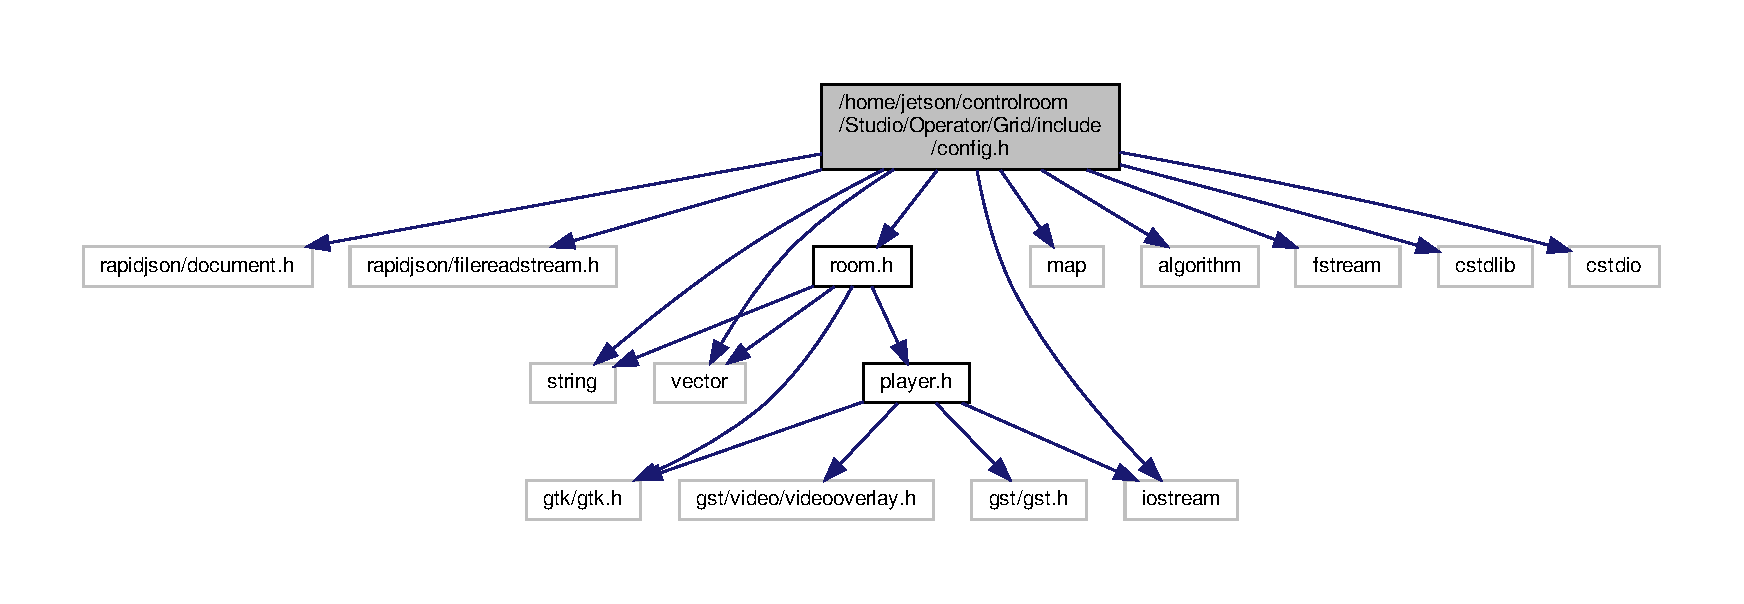
\includegraphics[width=350pt]{_operator_2_grid_2include_2config_8h__incl}
\end{center}
\end{figure}
Граф файлов, в которые включается этот файл\+:
\nopagebreak
\begin{figure}[H]
\begin{center}
\leavevmode
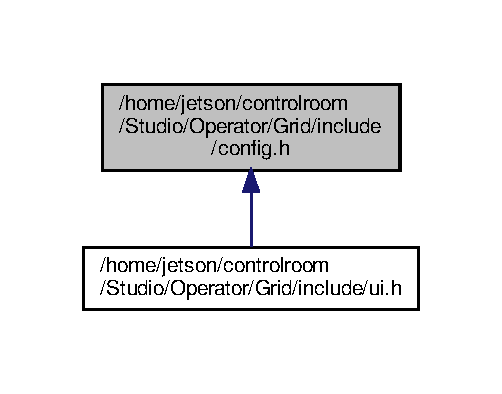
\includegraphics[width=241pt]{_operator_2_grid_2include_2config_8h__dep__incl}
\end{center}
\end{figure}
\subsection*{Классы}
\begin{DoxyCompactItemize}
\item 
class \hyperlink{class_config}{Config}
\begin{DoxyCompactList}\small\item\em The \hyperlink{class_config}{Config} class. \end{DoxyCompactList}\end{DoxyCompactItemize}

\hypertarget{_recorder_2include_2config_8h}{}\section{Файл /home/jetson/controlroom/\+Studio/\+Recorder/include/config.h}
\label{_recorder_2include_2config_8h}\index{/home/jetson/controlroom/\+Studio/\+Recorder/include/config.\+h@{/home/jetson/controlroom/\+Studio/\+Recorder/include/config.\+h}}
{\ttfamily \#include \char`\"{}rapidjson/document.\+h\char`\"{}}\newline
{\ttfamily \#include \char`\"{}room.\+h\char`\"{}}\newline
{\ttfamily \#include $<$vector$>$}\newline
{\ttfamily \#include $<$map$>$}\newline
{\ttfamily \#include $<$string$>$}\newline
{\ttfamily \#include $<$algorithm$>$}\newline
{\ttfamily \#include $<$fstream$>$}\newline
{\ttfamily \#include $<$iostream$>$}\newline
{\ttfamily \#include $<$cstdlib$>$}\newline
Граф включаемых заголовочных файлов для config.\+h\+:\nopagebreak
\begin{figure}[H]
\begin{center}
\leavevmode
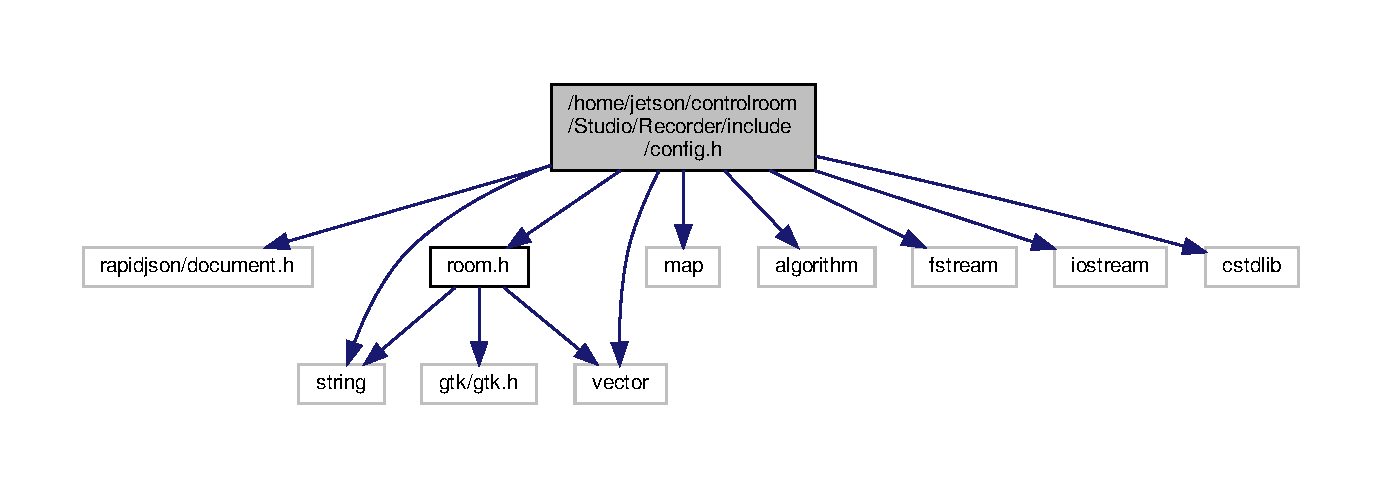
\includegraphics[width=350pt]{_recorder_2include_2config_8h__incl}
\end{center}
\end{figure}
Граф файлов, в которые включается этот файл\+:\nopagebreak
\begin{figure}[H]
\begin{center}
\leavevmode
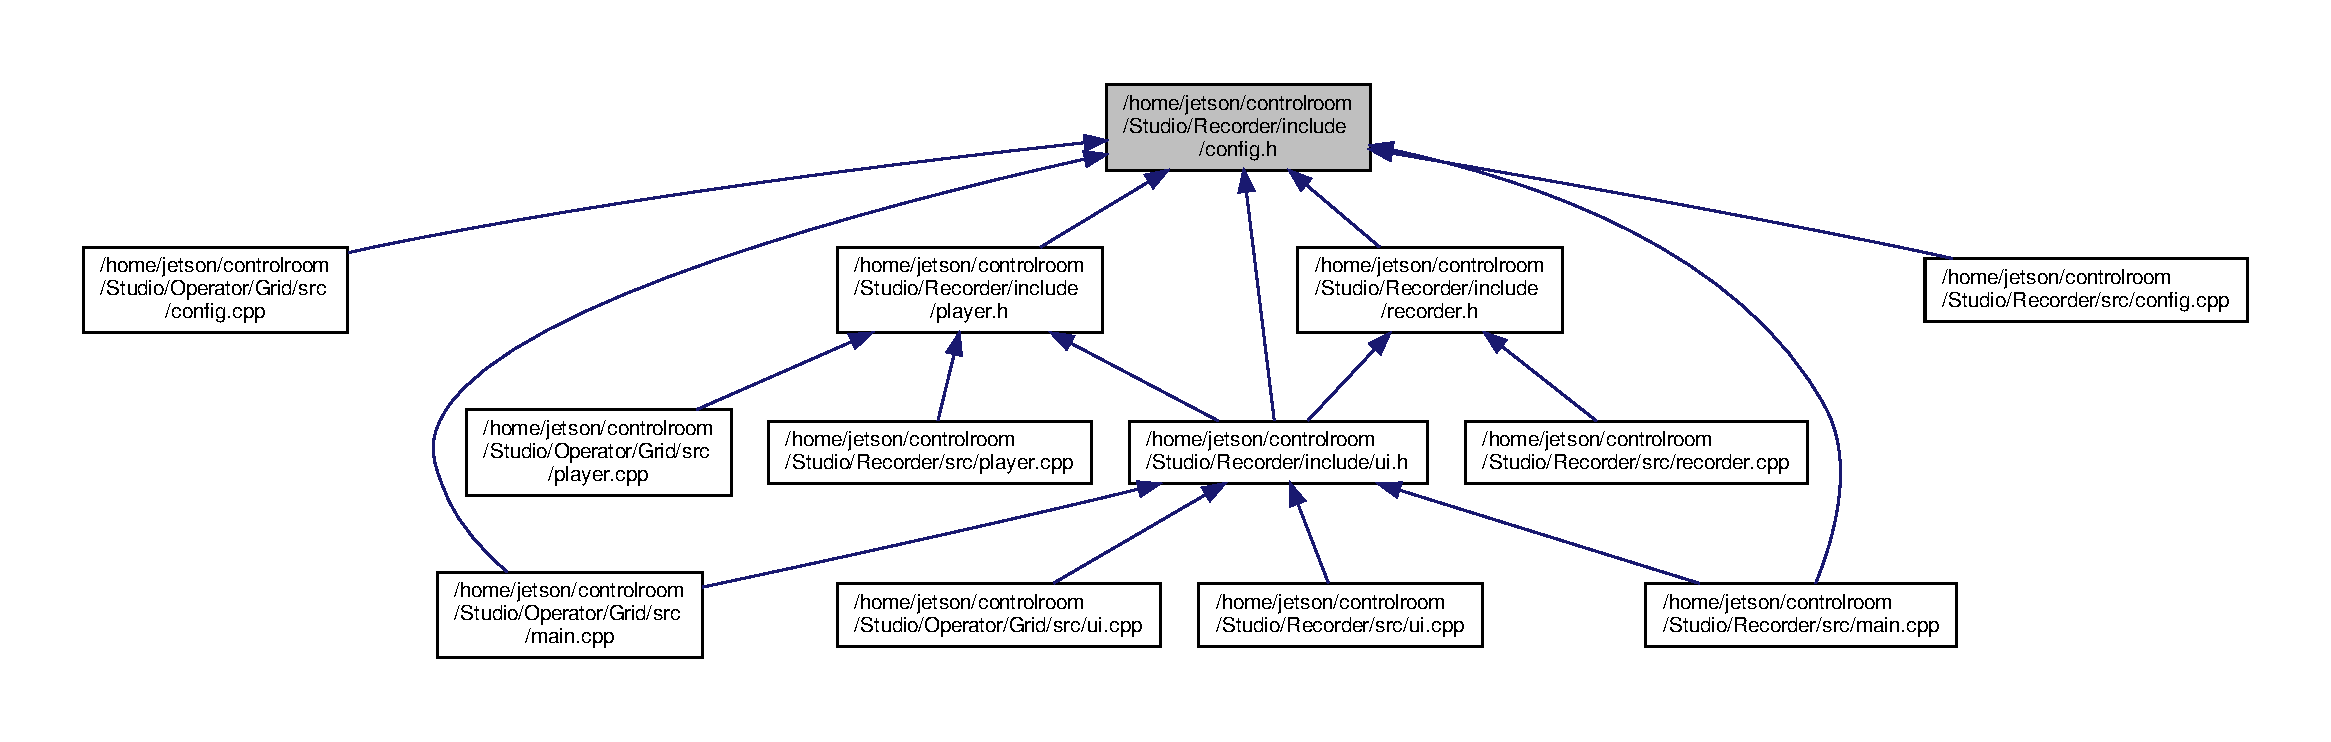
\includegraphics[width=350pt]{_recorder_2include_2config_8h__dep__incl}
\end{center}
\end{figure}
\subsection*{Классы}
\begin{DoxyCompactItemize}
\item 
class \hyperlink{class_config}{Config}
\begin{DoxyCompactList}\small\item\em The \hyperlink{class_config}{Config} class. \end{DoxyCompactList}\end{DoxyCompactItemize}

\hypertarget{_operator_2_grid_2include_2player_8h}{}\section{Файл /home/jetson/controlroom/\+Studio/\+Operator/\+Grid/include/player.h}
\label{_operator_2_grid_2include_2player_8h}\index{/home/jetson/controlroom/\+Studio/\+Operator/\+Grid/include/player.\+h@{/home/jetson/controlroom/\+Studio/\+Operator/\+Grid/include/player.\+h}}
{\ttfamily \#include $<$gtk/gtk.\+h$>$}\newline
{\ttfamily \#include $<$gst/gst.\+h$>$}\newline
{\ttfamily \#include $<$gst/video/videooverlay.\+h$>$}\newline
{\ttfamily \#include $<$iostream$>$}\newline
Граф включаемых заголовочных файлов для player.\+h\+:\nopagebreak
\begin{figure}[H]
\begin{center}
\leavevmode
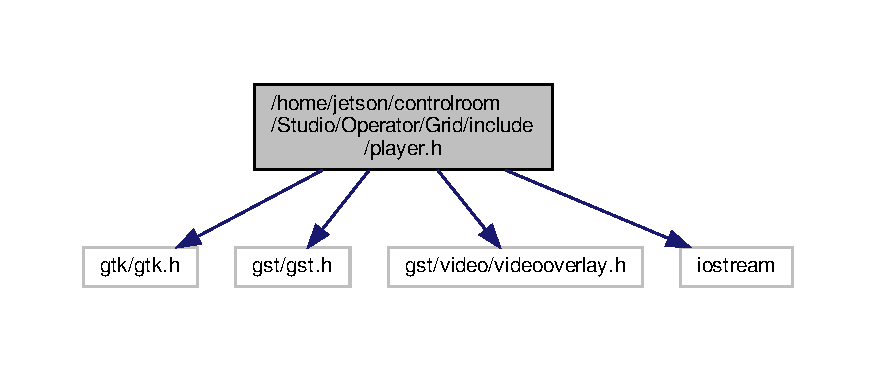
\includegraphics[width=350pt]{_operator_2_grid_2include_2player_8h__incl}
\end{center}
\end{figure}
Граф файлов, в которые включается этот файл\+:\nopagebreak
\begin{figure}[H]
\begin{center}
\leavevmode
\includegraphics[width=332pt]{_operator_2_grid_2include_2player_8h__dep__incl}
\end{center}
\end{figure}
\subsection*{Классы}
\begin{DoxyCompactItemize}
\item 
struct \hyperlink{struct_pad_data}{Pad\+Data}
\item 
class \hyperlink{class_player}{Player}
\begin{DoxyCompactList}\small\item\em The \hyperlink{class_player}{Player} class. \end{DoxyCompactList}\end{DoxyCompactItemize}

\hypertarget{_recorder_2include_2player_8h}{}\section{Файл /home/jetson/controlroom/\+Studio/\+Recorder/include/player.h}
\label{_recorder_2include_2player_8h}\index{/home/jetson/controlroom/\+Studio/\+Recorder/include/player.\+h@{/home/jetson/controlroom/\+Studio/\+Recorder/include/player.\+h}}
{\ttfamily \#include $<$gtk/gtk.\+h$>$}\newline
{\ttfamily \#include $<$gst/gst.\+h$>$}\newline
{\ttfamily \#include $<$gst/video/videooverlay.\+h$>$}\newline
{\ttfamily \#include \char`\"{}config.\+h\char`\"{}}\newline
Граф включаемых заголовочных файлов для player.\+h\+:\nopagebreak
\begin{figure}[H]
\begin{center}
\leavevmode
\includegraphics[width=350pt]{_recorder_2include_2player_8h__incl}
\end{center}
\end{figure}
Граф файлов, в которые включается этот файл\+:\nopagebreak
\begin{figure}[H]
\begin{center}
\leavevmode
\includegraphics[width=350pt]{_recorder_2include_2player_8h__dep__incl}
\end{center}
\end{figure}
\subsection*{Классы}
\begin{DoxyCompactItemize}
\item 
struct \hyperlink{struct_pad_data}{Pad\+Data}
\item 
class \hyperlink{class_player}{Player}
\begin{DoxyCompactList}\small\item\em The \hyperlink{class_player}{Player} class. \end{DoxyCompactList}\end{DoxyCompactItemize}

\hypertarget{_operator_2_grid_2include_2room_8h}{}\section{Файл /home/jetson/controlroom/\+Studio/\+Operator/\+Grid/include/room.h}
\label{_operator_2_grid_2include_2room_8h}\index{/home/jetson/controlroom/\+Studio/\+Operator/\+Grid/include/room.\+h@{/home/jetson/controlroom/\+Studio/\+Operator/\+Grid/include/room.\+h}}
{\ttfamily \#include $<$string$>$}\newline
{\ttfamily \#include $<$vector$>$}\newline
{\ttfamily \#include $<$gtk/gtk.\+h$>$}\newline
{\ttfamily \#include $<$player.\+h$>$}\newline
Граф включаемых заголовочных файлов для room.\+h\+:\nopagebreak
\begin{figure}[H]
\begin{center}
\leavevmode
\includegraphics[width=350pt]{_operator_2_grid_2include_2room_8h__incl}
\end{center}
\end{figure}
Граф файлов, в которые включается этот файл\+:\nopagebreak
\begin{figure}[H]
\begin{center}
\leavevmode
\includegraphics[width=290pt]{_operator_2_grid_2include_2room_8h__dep__incl}
\end{center}
\end{figure}
\subsection*{Классы}
\begin{DoxyCompactItemize}
\item 
struct \hyperlink{struct_camera}{Camera}
\item 
struct \hyperlink{struct_audio_source}{Audio\+Source}
\item 
class \hyperlink{class_room}{Room}
\begin{DoxyCompactList}\small\item\em The \hyperlink{class_room}{Room} class. \end{DoxyCompactList}\end{DoxyCompactItemize}
\subsection*{Перечисления}
\begin{DoxyCompactItemize}
\item 
enum \hyperlink{_operator_2_grid_2include_2room_8h_aba46c5e77984ba564800a07427f8eeb1}{room\+\_\+t} \{ \hyperlink{_operator_2_grid_2include_2room_8h_aba46c5e77984ba564800a07427f8eeb1a945d6010d321d9fe75cbba7b6f37f3b5}{C\+U\+S\+T\+OM}, 
\hyperlink{_operator_2_grid_2include_2room_8h_aba46c5e77984ba564800a07427f8eeb1af3becc2ef5d63e47f97c711e7a49fc5a}{G\+S\+U\+I\+TE}, 
\hyperlink{_recorder_2include_2room_8h_aba46c5e77984ba564800a07427f8eeb1a945d6010d321d9fe75cbba7b6f37f3b5}{C\+U\+S\+T\+OM}, 
\hyperlink{_recorder_2include_2room_8h_aba46c5e77984ba564800a07427f8eeb1af3becc2ef5d63e47f97c711e7a49fc5a}{G\+S\+U\+I\+TE}
 \}
\end{DoxyCompactItemize}


\subsection{Перечисления}
\mbox{\Hypertarget{_operator_2_grid_2include_2room_8h_aba46c5e77984ba564800a07427f8eeb1}\label{_operator_2_grid_2include_2room_8h_aba46c5e77984ba564800a07427f8eeb1}} 
\index{Operator/\+Grid/include/room.\+h@{Operator/\+Grid/include/room.\+h}!room\+\_\+t@{room\+\_\+t}}
\index{room\+\_\+t@{room\+\_\+t}!Operator/\+Grid/include/room.\+h@{Operator/\+Grid/include/room.\+h}}
\subsubsection{\texorpdfstring{room\+\_\+t}{room\_t}}
{\footnotesize\ttfamily enum \hyperlink{_operator_2_grid_2include_2room_8h_aba46c5e77984ba564800a07427f8eeb1}{room\+\_\+t}}

\begin{DoxyEnumFields}{Элементы перечислений}
\raisebox{\heightof{T}}[0pt][0pt]{\index{C\+U\+S\+T\+OM@{C\+U\+S\+T\+OM}!Operator/\+Grid/include/room.\+h@{Operator/\+Grid/include/room.\+h}}\index{Operator/\+Grid/include/room.\+h@{Operator/\+Grid/include/room.\+h}!C\+U\+S\+T\+OM@{C\+U\+S\+T\+OM}}}\mbox{\Hypertarget{_operator_2_grid_2include_2room_8h_aba46c5e77984ba564800a07427f8eeb1a945d6010d321d9fe75cbba7b6f37f3b5}\label{_operator_2_grid_2include_2room_8h_aba46c5e77984ba564800a07427f8eeb1a945d6010d321d9fe75cbba7b6f37f3b5}} 
C\+U\+S\+T\+OM&\\
\hline

\raisebox{\heightof{T}}[0pt][0pt]{\index{G\+S\+U\+I\+TE@{G\+S\+U\+I\+TE}!Operator/\+Grid/include/room.\+h@{Operator/\+Grid/include/room.\+h}}\index{Operator/\+Grid/include/room.\+h@{Operator/\+Grid/include/room.\+h}!G\+S\+U\+I\+TE@{G\+S\+U\+I\+TE}}}\mbox{\Hypertarget{_operator_2_grid_2include_2room_8h_aba46c5e77984ba564800a07427f8eeb1af3becc2ef5d63e47f97c711e7a49fc5a}\label{_operator_2_grid_2include_2room_8h_aba46c5e77984ba564800a07427f8eeb1af3becc2ef5d63e47f97c711e7a49fc5a}} 
G\+S\+U\+I\+TE&\\
\hline

\raisebox{\heightof{T}}[0pt][0pt]{\index{C\+U\+S\+T\+OM@{C\+U\+S\+T\+OM}!Operator/\+Grid/include/room.\+h@{Operator/\+Grid/include/room.\+h}}\index{Operator/\+Grid/include/room.\+h@{Operator/\+Grid/include/room.\+h}!C\+U\+S\+T\+OM@{C\+U\+S\+T\+OM}}}\mbox{\Hypertarget{_operator_2_grid_2include_2room_8h_aba46c5e77984ba564800a07427f8eeb1a945d6010d321d9fe75cbba7b6f37f3b5}\label{_operator_2_grid_2include_2room_8h_aba46c5e77984ba564800a07427f8eeb1a945d6010d321d9fe75cbba7b6f37f3b5}} 
C\+U\+S\+T\+OM&\\
\hline

\raisebox{\heightof{T}}[0pt][0pt]{\index{G\+S\+U\+I\+TE@{G\+S\+U\+I\+TE}!Operator/\+Grid/include/room.\+h@{Operator/\+Grid/include/room.\+h}}\index{Operator/\+Grid/include/room.\+h@{Operator/\+Grid/include/room.\+h}!G\+S\+U\+I\+TE@{G\+S\+U\+I\+TE}}}\mbox{\Hypertarget{_operator_2_grid_2include_2room_8h_aba46c5e77984ba564800a07427f8eeb1af3becc2ef5d63e47f97c711e7a49fc5a}\label{_operator_2_grid_2include_2room_8h_aba46c5e77984ba564800a07427f8eeb1af3becc2ef5d63e47f97c711e7a49fc5a}} 
G\+S\+U\+I\+TE&\\
\hline

\end{DoxyEnumFields}

\hypertarget{_recorder_2include_2room_8h}{}\section{Файл /home/jetson/controlroom/\+Studio/\+Recorder/include/room.h}
\label{_recorder_2include_2room_8h}\index{/home/jetson/controlroom/\+Studio/\+Recorder/include/room.\+h@{/home/jetson/controlroom/\+Studio/\+Recorder/include/room.\+h}}
{\ttfamily \#include $<$string$>$}\newline
{\ttfamily \#include $<$vector$>$}\newline
{\ttfamily \#include $<$gtk/gtk.\+h$>$}\newline
Граф включаемых заголовочных файлов для room.\+h\+:\nopagebreak
\begin{figure}[H]
\begin{center}
\leavevmode
\includegraphics[width=257pt]{_recorder_2include_2room_8h__incl}
\end{center}
\end{figure}
Граф файлов, в которые включается этот файл\+:\nopagebreak
\begin{figure}[H]
\begin{center}
\leavevmode
\includegraphics[width=350pt]{_recorder_2include_2room_8h__dep__incl}
\end{center}
\end{figure}
\subsection*{Классы}
\begin{DoxyCompactItemize}
\item 
struct \hyperlink{struct_camera}{Camera}
\item 
struct \hyperlink{struct_audio_source}{Audio\+Source}
\item 
class \hyperlink{class_room}{Room}
\begin{DoxyCompactList}\small\item\em The \hyperlink{class_room}{Room} class. \end{DoxyCompactList}\end{DoxyCompactItemize}
\subsection*{Перечисления}
\begin{DoxyCompactItemize}
\item 
enum \hyperlink{_recorder_2include_2room_8h_aba46c5e77984ba564800a07427f8eeb1}{room\+\_\+t} \{ \hyperlink{_operator_2_grid_2include_2room_8h_aba46c5e77984ba564800a07427f8eeb1a945d6010d321d9fe75cbba7b6f37f3b5}{C\+U\+S\+T\+OM}, 
\hyperlink{_operator_2_grid_2include_2room_8h_aba46c5e77984ba564800a07427f8eeb1af3becc2ef5d63e47f97c711e7a49fc5a}{G\+S\+U\+I\+TE}, 
\hyperlink{_recorder_2include_2room_8h_aba46c5e77984ba564800a07427f8eeb1a945d6010d321d9fe75cbba7b6f37f3b5}{C\+U\+S\+T\+OM}, 
\hyperlink{_recorder_2include_2room_8h_aba46c5e77984ba564800a07427f8eeb1af3becc2ef5d63e47f97c711e7a49fc5a}{G\+S\+U\+I\+TE}
 \}
\end{DoxyCompactItemize}


\subsection{Перечисления}
\mbox{\Hypertarget{_recorder_2include_2room_8h_aba46c5e77984ba564800a07427f8eeb1}\label{_recorder_2include_2room_8h_aba46c5e77984ba564800a07427f8eeb1}} 
\index{Recorder/include/room.\+h@{Recorder/include/room.\+h}!room\+\_\+t@{room\+\_\+t}}
\index{room\+\_\+t@{room\+\_\+t}!Recorder/include/room.\+h@{Recorder/include/room.\+h}}
\subsubsection{\texorpdfstring{room\+\_\+t}{room\_t}}
{\footnotesize\ttfamily enum \hyperlink{_operator_2_grid_2include_2room_8h_aba46c5e77984ba564800a07427f8eeb1}{room\+\_\+t}}

\begin{DoxyEnumFields}{Элементы перечислений}
\raisebox{\heightof{T}}[0pt][0pt]{\index{C\+U\+S\+T\+OM@{C\+U\+S\+T\+OM}!Recorder/include/room.\+h@{Recorder/include/room.\+h}}\index{Recorder/include/room.\+h@{Recorder/include/room.\+h}!C\+U\+S\+T\+OM@{C\+U\+S\+T\+OM}}}\mbox{\Hypertarget{_recorder_2include_2room_8h_aba46c5e77984ba564800a07427f8eeb1a945d6010d321d9fe75cbba7b6f37f3b5}\label{_recorder_2include_2room_8h_aba46c5e77984ba564800a07427f8eeb1a945d6010d321d9fe75cbba7b6f37f3b5}} 
C\+U\+S\+T\+OM&\\
\hline

\raisebox{\heightof{T}}[0pt][0pt]{\index{G\+S\+U\+I\+TE@{G\+S\+U\+I\+TE}!Recorder/include/room.\+h@{Recorder/include/room.\+h}}\index{Recorder/include/room.\+h@{Recorder/include/room.\+h}!G\+S\+U\+I\+TE@{G\+S\+U\+I\+TE}}}\mbox{\Hypertarget{_recorder_2include_2room_8h_aba46c5e77984ba564800a07427f8eeb1af3becc2ef5d63e47f97c711e7a49fc5a}\label{_recorder_2include_2room_8h_aba46c5e77984ba564800a07427f8eeb1af3becc2ef5d63e47f97c711e7a49fc5a}} 
G\+S\+U\+I\+TE&\\
\hline

\raisebox{\heightof{T}}[0pt][0pt]{\index{C\+U\+S\+T\+OM@{C\+U\+S\+T\+OM}!Recorder/include/room.\+h@{Recorder/include/room.\+h}}\index{Recorder/include/room.\+h@{Recorder/include/room.\+h}!C\+U\+S\+T\+OM@{C\+U\+S\+T\+OM}}}\mbox{\Hypertarget{_recorder_2include_2room_8h_aba46c5e77984ba564800a07427f8eeb1a945d6010d321d9fe75cbba7b6f37f3b5}\label{_recorder_2include_2room_8h_aba46c5e77984ba564800a07427f8eeb1a945d6010d321d9fe75cbba7b6f37f3b5}} 
C\+U\+S\+T\+OM&\\
\hline

\raisebox{\heightof{T}}[0pt][0pt]{\index{G\+S\+U\+I\+TE@{G\+S\+U\+I\+TE}!Recorder/include/room.\+h@{Recorder/include/room.\+h}}\index{Recorder/include/room.\+h@{Recorder/include/room.\+h}!G\+S\+U\+I\+TE@{G\+S\+U\+I\+TE}}}\mbox{\Hypertarget{_recorder_2include_2room_8h_aba46c5e77984ba564800a07427f8eeb1af3becc2ef5d63e47f97c711e7a49fc5a}\label{_recorder_2include_2room_8h_aba46c5e77984ba564800a07427f8eeb1af3becc2ef5d63e47f97c711e7a49fc5a}} 
G\+S\+U\+I\+TE&\\
\hline

\end{DoxyEnumFields}

\hypertarget{_operator_2_grid_2include_2ui_8h}{}\section{Файл /home/jetson/controlroom/\+Studio/\+Operator/\+Grid/include/ui.h}
\label{_operator_2_grid_2include_2ui_8h}\index{/home/jetson/controlroom/\+Studio/\+Operator/\+Grid/include/ui.\+h@{/home/jetson/controlroom/\+Studio/\+Operator/\+Grid/include/ui.\+h}}
{\ttfamily \#include \char`\"{}config.\+h\char`\"{}}\newline
{\ttfamily \#include $<$iostream$>$}\newline
{\ttfamily \#include $<$string$>$}\newline
{\ttfamily \#include $<$unistd.\+h$>$}\newline
{\ttfamily \#include $<$gtk/gtk.\+h$>$}\newline
{\ttfamily \#include $<$gdk/gdk.\+h$>$}\newline
{\ttfamily \#include \char`\"{}room.\+h\char`\"{}}\newline
{\ttfamily \#include \char`\"{}player.\+h\char`\"{}}\newline
{\ttfamily \#include $<$cstdlib$>$}\newline
{\ttfamily \#include $<$netdb.\+h$>$}\newline
{\ttfamily \#include $<$sys/types.\+h$>$}\newline
{\ttfamily \#include $<$sys/socket.\+h$>$}\newline
{\ttfamily \#include $<$netinet/in.\+h$>$}\newline
{\ttfamily \#include $<$arpa/inet.\+h$>$}\newline
Граф включаемых заголовочных файлов для ui.\+h\+:
\nopagebreak
\begin{figure}[H]
\begin{center}
\leavevmode
\includegraphics[width=350pt]{_operator_2_grid_2include_2ui_8h__incl}
\end{center}
\end{figure}
\subsection*{Классы}
\begin{DoxyCompactItemize}
\item 
class \hyperlink{class_u_i}{UI}
\begin{DoxyCompactList}\small\item\em The \hyperlink{class_u_i}{UI} class. \end{DoxyCompactList}\item 
struct \hyperlink{struct_u_i_1_1display__player__data}{U\+I\+::display\+\_\+player\+\_\+data}
\end{DoxyCompactItemize}

\hypertarget{_recorder_2include_2ui_8h}{}\section{Файл /home/jetson/controlroom/\+Studio/\+Recorder/include/ui.h}
\label{_recorder_2include_2ui_8h}\index{/home/jetson/controlroom/\+Studio/\+Recorder/include/ui.\+h@{/home/jetson/controlroom/\+Studio/\+Recorder/include/ui.\+h}}
{\ttfamily \#include $<$iostream$>$}\newline
{\ttfamily \#include $<$string$>$}\newline
{\ttfamily \#include $<$unistd.\+h$>$}\newline
{\ttfamily \#include $<$gtk/gtk.\+h$>$}\newline
{\ttfamily \#include $<$gdk/gdk.\+h$>$}\newline
{\ttfamily \#include \char`\"{}room.\+h\char`\"{}}\newline
{\ttfamily \#include \char`\"{}config.\+h\char`\"{}}\newline
{\ttfamily \#include \char`\"{}player.\+h\char`\"{}}\newline
{\ttfamily \#include \char`\"{}recorder.\+h\char`\"{}}\newline
{\ttfamily \#include $<$cstdlib$>$}\newline
{\ttfamily \#include $<$netdb.\+h$>$}\newline
{\ttfamily \#include $<$sys/types.\+h$>$}\newline
{\ttfamily \#include $<$sys/socket.\+h$>$}\newline
{\ttfamily \#include $<$netinet/in.\+h$>$}\newline
{\ttfamily \#include $<$arpa/inet.\+h$>$}\newline
{\ttfamily \#include $<$sys/statvfs.\+h$>$}\newline
{\ttfamily \#include $<$iomanip$>$}\newline
Граф включаемых заголовочных файлов для ui.\+h\+:\nopagebreak
\begin{figure}[H]
\begin{center}
\leavevmode
\includegraphics[width=350pt]{_recorder_2include_2ui_8h__incl}
\end{center}
\end{figure}
Граф файлов, в которые включается этот файл\+:\nopagebreak
\begin{figure}[H]
\begin{center}
\leavevmode
\includegraphics[width=350pt]{_recorder_2include_2ui_8h__dep__incl}
\end{center}
\end{figure}
\subsection*{Классы}
\begin{DoxyCompactItemize}
\item 
class \hyperlink{class_u_i}{UI}
\begin{DoxyCompactList}\small\item\em The \hyperlink{class_u_i}{UI} class. \end{DoxyCompactList}\item 
struct \hyperlink{struct_u_i_1_1gdrive__status__data}{U\+I\+::gdrive\+\_\+status\+\_\+data}
\item 
struct \hyperlink{struct_u_i_1_1display__player__data}{U\+I\+::display\+\_\+player\+\_\+data}
\item 
struct \hyperlink{struct_u_i_1_1switch__state__changed__data}{U\+I\+::switch\+\_\+state\+\_\+changed\+\_\+data}
\end{DoxyCompactItemize}

\hypertarget{_operator_2_grid_2src_2config_8cpp}{}\section{Файл /home/jetson/controlroom/\+Studio/\+Operator/\+Grid/src/config.cpp}
\label{_operator_2_grid_2src_2config_8cpp}\index{/home/jetson/controlroom/\+Studio/\+Operator/\+Grid/src/config.\+cpp@{/home/jetson/controlroom/\+Studio/\+Operator/\+Grid/src/config.\+cpp}}
{\ttfamily \#include \char`\"{}config.\+h\char`\"{}}\newline
Граф включаемых заголовочных файлов для config.\+cpp\+:\nopagebreak
\begin{figure}[H]
\begin{center}
\leavevmode
\includegraphics[width=207pt]{_operator_2_grid_2src_2config_8cpp__incl}
\end{center}
\end{figure}

\hypertarget{_recorder_2src_2config_8cpp}{}\section{Файл /home/jetson/controlroom/\+Studio/\+Recorder/src/config.cpp}
\label{_recorder_2src_2config_8cpp}\index{/home/jetson/controlroom/\+Studio/\+Recorder/src/config.\+cpp@{/home/jetson/controlroom/\+Studio/\+Recorder/src/config.\+cpp}}
{\ttfamily \#include \char`\"{}config.\+h\char`\"{}}\newline
Граф включаемых заголовочных файлов для config.\+cpp\+:\nopagebreak
\begin{figure}[H]
\begin{center}
\leavevmode
\includegraphics[width=235pt]{_recorder_2src_2config_8cpp__incl}
\end{center}
\end{figure}

\hypertarget{_operator_2_grid_2src_2from-gsuite_8py}{}\section{Файл /home/jetson/controlroom/\+Studio/\+Operator/\+Grid/src/from-\/gsuite.py}
\label{_operator_2_grid_2src_2from-gsuite_8py}\index{/home/jetson/controlroom/\+Studio/\+Operator/\+Grid/src/from-\/gsuite.\+py@{/home/jetson/controlroom/\+Studio/\+Operator/\+Grid/src/from-\/gsuite.\+py}}
\subsection*{Пространства имен}
\begin{DoxyCompactItemize}
\item 
 \hyperlink{namespacefrom-gsuite}{from-\/gsuite}
\end{DoxyCompactItemize}
\subsection*{Функции}
\begin{DoxyCompactItemize}
\item 
def \hyperlink{namespacefrom-gsuite_a431d5ae5f08baa594842e68180930f6c}{from-\/gsuite.\+main} ()
\end{DoxyCompactItemize}
\subsection*{Переменные}
\begin{DoxyCompactItemize}
\item 
list \hyperlink{namespacefrom-gsuite_a359fb1aa3ebe4472fff6f682676e7dc0}{from-\/gsuite.\+S\+C\+O\+P\+ES} = \mbox{[}\textquotesingle{}https\+://www.\+googleapis.\+com/auth/admin.\+directory.\+resource.\+calendar\textquotesingle{}\mbox{]}
\end{DoxyCompactItemize}

\hypertarget{_recorder_2src_2from-gsuite_8py}{}\section{Файл /home/jetson/controlroom/\+Studio/\+Recorder/src/from-\/gsuite.py}
\label{_recorder_2src_2from-gsuite_8py}\index{/home/jetson/controlroom/\+Studio/\+Recorder/src/from-\/gsuite.\+py@{/home/jetson/controlroom/\+Studio/\+Recorder/src/from-\/gsuite.\+py}}
\subsection*{Пространства имен}
\begin{DoxyCompactItemize}
\item 
 \hyperlink{namespacefrom-gsuite}{from-\/gsuite}
\end{DoxyCompactItemize}
\subsection*{Функции}
\begin{DoxyCompactItemize}
\item 
def \hyperlink{namespacefrom-gsuite_a431d5ae5f08baa594842e68180930f6c}{from-\/gsuite.\+main} ()
\end{DoxyCompactItemize}

\hypertarget{_operator_2_grid_2src_2main_8cpp}{}\section{Файл /home/jetson/controlroom/\+Studio/\+Operator/\+Grid/src/main.cpp}
\label{_operator_2_grid_2src_2main_8cpp}\index{/home/jetson/controlroom/\+Studio/\+Operator/\+Grid/src/main.\+cpp@{/home/jetson/controlroom/\+Studio/\+Operator/\+Grid/src/main.\+cpp}}
{\ttfamily \#include \char`\"{}config.\+h\char`\"{}}\newline
{\ttfamily \#include $<$iostream$>$}\newline
{\ttfamily \#include $<$string$>$}\newline
{\ttfamily \#include $<$cstdio$>$}\newline
{\ttfamily \#include \char`\"{}ui.\+h\char`\"{}}\newline
Граф включаемых заголовочных файлов для main.\+cpp\+:\nopagebreak
\begin{figure}[H]
\begin{center}
\leavevmode
\includegraphics[width=350pt]{_operator_2_grid_2src_2main_8cpp__incl}
\end{center}
\end{figure}
\subsection*{Функции}
\begin{DoxyCompactItemize}
\item 
int \hyperlink{_operator_2_grid_2src_2main_8cpp_ae66f6b31b5ad750f1fe042a706a4e3d4}{main} ()
\end{DoxyCompactItemize}


\subsection{Функции}
\mbox{\Hypertarget{_operator_2_grid_2src_2main_8cpp_ae66f6b31b5ad750f1fe042a706a4e3d4}\label{_operator_2_grid_2src_2main_8cpp_ae66f6b31b5ad750f1fe042a706a4e3d4}} 
\index{Operator/\+Grid/src/main.\+cpp@{Operator/\+Grid/src/main.\+cpp}!main@{main}}
\index{main@{main}!Operator/\+Grid/src/main.\+cpp@{Operator/\+Grid/src/main.\+cpp}}
\subsubsection{\texorpdfstring{main()}{main()}}
{\footnotesize\ttfamily int main (\begin{DoxyParamCaption}{ }\end{DoxyParamCaption})}

Граф вызовов\+:\nopagebreak
\begin{figure}[H]
\begin{center}
\leavevmode
\includegraphics[width=234pt]{_operator_2_grid_2src_2main_8cpp_ae66f6b31b5ad750f1fe042a706a4e3d4_cgraph}
\end{center}
\end{figure}

\hypertarget{_recorder_2src_2main_8cpp}{}\section{Файл /home/jetson/controlroom/\+Studio/\+Recorder/src/main.cpp}
\label{_recorder_2src_2main_8cpp}\index{/home/jetson/controlroom/\+Studio/\+Recorder/src/main.\+cpp@{/home/jetson/controlroom/\+Studio/\+Recorder/src/main.\+cpp}}
{\ttfamily \#include $<$iostream$>$}\newline
{\ttfamily \#include $<$string$>$}\newline
{\ttfamily \#include $<$cstdio$>$}\newline
{\ttfamily \#include \char`\"{}ui.\+h\char`\"{}}\newline
{\ttfamily \#include \char`\"{}config.\+h\char`\"{}}\newline
Граф включаемых заголовочных файлов для main.\+cpp\+:\nopagebreak
\begin{figure}[H]
\begin{center}
\leavevmode
\includegraphics[width=350pt]{_recorder_2src_2main_8cpp__incl}
\end{center}
\end{figure}
\subsection*{Функции}
\begin{DoxyCompactItemize}
\item 
int \hyperlink{_recorder_2src_2main_8cpp_ae66f6b31b5ad750f1fe042a706a4e3d4}{main} ()
\end{DoxyCompactItemize}


\subsection{Функции}
\mbox{\Hypertarget{_recorder_2src_2main_8cpp_ae66f6b31b5ad750f1fe042a706a4e3d4}\label{_recorder_2src_2main_8cpp_ae66f6b31b5ad750f1fe042a706a4e3d4}} 
\index{Recorder/src/main.\+cpp@{Recorder/src/main.\+cpp}!main@{main}}
\index{main@{main}!Recorder/src/main.\+cpp@{Recorder/src/main.\+cpp}}
\subsubsection{\texorpdfstring{main()}{main()}}
{\footnotesize\ttfamily int main (\begin{DoxyParamCaption}{ }\end{DoxyParamCaption})}

Граф вызовов\+:\nopagebreak
\begin{figure}[H]
\begin{center}
\leavevmode
\includegraphics[width=234pt]{_recorder_2src_2main_8cpp_ae66f6b31b5ad750f1fe042a706a4e3d4_cgraph}
\end{center}
\end{figure}

\hypertarget{_operator_2_grid_2src_2player_8cpp}{}\section{Файл /home/jetson/controlroom/\+Studio/\+Operator/\+Grid/src/player.cpp}
\label{_operator_2_grid_2src_2player_8cpp}\index{/home/jetson/controlroom/\+Studio/\+Operator/\+Grid/src/player.\+cpp@{/home/jetson/controlroom/\+Studio/\+Operator/\+Grid/src/player.\+cpp}}
{\ttfamily \#include \char`\"{}player.\+h\char`\"{}}\newline
Граф включаемых заголовочных файлов для player.\+cpp\+:\nopagebreak
\begin{figure}[H]
\begin{center}
\leavevmode
\includegraphics[width=207pt]{_operator_2_grid_2src_2player_8cpp__incl}
\end{center}
\end{figure}

\hypertarget{_recorder_2src_2player_8cpp}{}\section{Файл /home/jetson/controlroom/\+Studio/\+Recorder/src/player.cpp}
\label{_recorder_2src_2player_8cpp}\index{/home/jetson/controlroom/\+Studio/\+Recorder/src/player.\+cpp@{/home/jetson/controlroom/\+Studio/\+Recorder/src/player.\+cpp}}
{\ttfamily \#include \char`\"{}player.\+h\char`\"{}}\newline
Граф включаемых заголовочных файлов для player.\+cpp\+:\nopagebreak
\begin{figure}[H]
\begin{center}
\leavevmode
\includegraphics[width=235pt]{_recorder_2src_2player_8cpp__incl}
\end{center}
\end{figure}

\hypertarget{_operator_2_grid_2src_2ui_8cpp}{}\section{Файл /home/jetson/controlroom/\+Studio/\+Operator/\+Grid/src/ui.cpp}
\label{_operator_2_grid_2src_2ui_8cpp}\index{/home/jetson/controlroom/\+Studio/\+Operator/\+Grid/src/ui.\+cpp@{/home/jetson/controlroom/\+Studio/\+Operator/\+Grid/src/ui.\+cpp}}
{\ttfamily \#include \char`\"{}ui.\+h\char`\"{}}\newline
Граф включаемых заголовочных файлов для ui.\+cpp\+:\nopagebreak
\begin{figure}[H]
\begin{center}
\leavevmode
\includegraphics[width=235pt]{_operator_2_grid_2src_2ui_8cpp__incl}
\end{center}
\end{figure}

\hypertarget{_recorder_2src_2ui_8cpp}{}\section{Файл /home/jetson/controlroom/\+Studio/\+Recorder/src/ui.cpp}
\label{_recorder_2src_2ui_8cpp}\index{/home/jetson/controlroom/\+Studio/\+Recorder/src/ui.\+cpp@{/home/jetson/controlroom/\+Studio/\+Recorder/src/ui.\+cpp}}
{\ttfamily \#include \char`\"{}ui.\+h\char`\"{}}\newline
Граф включаемых заголовочных файлов для ui.\+cpp\+:\nopagebreak
\begin{figure}[H]
\begin{center}
\leavevmode
\includegraphics[width=216pt]{_recorder_2src_2ui_8cpp__incl}
\end{center}
\end{figure}

\hypertarget{recorder_8h}{}\section{Файл /home/jetson/controlroom/\+Studio/\+Recorder/include/recorder.h}
\label{recorder_8h}\index{/home/jetson/controlroom/\+Studio/\+Recorder/include/recorder.\+h@{/home/jetson/controlroom/\+Studio/\+Recorder/include/recorder.\+h}}
{\ttfamily \#include $<$iostream$>$}\newline
{\ttfamily \#include $<$vector$>$}\newline
{\ttfamily \#include $<$string$>$}\newline
{\ttfamily \#include $<$signal.\+h$>$}\newline
{\ttfamily \#include $<$unistd.\+h$>$}\newline
{\ttfamily \#include $<$fcntl.\+h$>$}\newline
{\ttfamily \#include $<$wait.\+h$>$}\newline
{\ttfamily \#include \char`\"{}config.\+h\char`\"{}}\newline
{\ttfamily \#include $<$ctime$>$}\newline
{\ttfamily \#include $<$cstring$>$}\newline
{\ttfamily \#include $<$stdlib.\+h$>$}\newline
{\ttfamily \#include $<$stdio.\+h$>$}\newline
{\ttfamily \#include $<$cstdlib$>$}\newline
{\ttfamily \#include $<$bits/stdc++.\+h$>$}\newline
{\ttfamily \#include \char`\"{}recording.\+h\char`\"{}}\newline
{\ttfamily \#include \char`\"{}room.\+h\char`\"{}}\newline
Граф включаемых заголовочных файлов для recorder.\+h\+:\nopagebreak
\begin{figure}[H]
\begin{center}
\leavevmode
\includegraphics[width=350pt]{recorder_8h__incl}
\end{center}
\end{figure}
Граф файлов, в которые включается этот файл\+:\nopagebreak
\begin{figure}[H]
\begin{center}
\leavevmode
\includegraphics[width=350pt]{recorder_8h__dep__incl}
\end{center}
\end{figure}
\subsection*{Классы}
\begin{DoxyCompactItemize}
\item 
class \hyperlink{class_recorder}{Recorder}
\begin{DoxyCompactList}\small\item\em Управляет процессом записи \end{DoxyCompactList}\end{DoxyCompactItemize}

\hypertarget{recording_8h}{}\section{Файл /home/jetson/controlroom/\+Studio/\+Recorder/include/recording.h}
\label{recording_8h}\index{/home/jetson/controlroom/\+Studio/\+Recorder/include/recording.\+h@{/home/jetson/controlroom/\+Studio/\+Recorder/include/recording.\+h}}
{\ttfamily \#include $<$string$>$}\newline
{\ttfamily \#include $<$gst/gst.\+h$>$}\newline
{\ttfamily \#include $<$iostream$>$}\newline
Граф включаемых заголовочных файлов для recording.\+h\+:\nopagebreak
\begin{figure}[H]
\begin{center}
\leavevmode
\includegraphics[width=267pt]{recording_8h__incl}
\end{center}
\end{figure}
Граф файлов, в которые включается этот файл\+:\nopagebreak
\begin{figure}[H]
\begin{center}
\leavevmode
\includegraphics[width=350pt]{recording_8h__dep__incl}
\end{center}
\end{figure}
\subsection*{Классы}
\begin{DoxyCompactItemize}
\item 
class \hyperlink{class_recording}{Recording}
\begin{DoxyCompactList}\small\item\em The \hyperlink{class_recording}{Recording} class. \end{DoxyCompactList}\end{DoxyCompactItemize}
\subsection*{Перечисления}
\begin{DoxyCompactItemize}
\item 
enum \hyperlink{recording_8h_af9bff8ff1154a04a899276af806b8586}{status\+\_\+t} \{ \hyperlink{recording_8h_af9bff8ff1154a04a899276af806b8586a1061be6c3fb88d32829cba6f6b2be304}{R\+U\+N\+N\+I\+NG}, 
\hyperlink{recording_8h_af9bff8ff1154a04a899276af806b8586a32fb07b4772ca4ee2861321344034f33}{R\+E\+L\+I\+N\+K\+I\+NG}, 
\hyperlink{recording_8h_af9bff8ff1154a04a899276af806b8586a898cbaf2e64179c5cfdff4d10b3728c1}{S\+T\+O\+P\+P\+I\+NG}, 
\hyperlink{recording_8h_af9bff8ff1154a04a899276af806b8586a948b2aee15f52b421fa4770c47bcfe8c}{S\+T\+O\+P\+P\+ED}
 \}
\end{DoxyCompactItemize}


\subsection{Перечисления}
\mbox{\Hypertarget{recording_8h_af9bff8ff1154a04a899276af806b8586}\label{recording_8h_af9bff8ff1154a04a899276af806b8586}} 
\index{recording.\+h@{recording.\+h}!status\+\_\+t@{status\+\_\+t}}
\index{status\+\_\+t@{status\+\_\+t}!recording.\+h@{recording.\+h}}
\subsubsection{\texorpdfstring{status\+\_\+t}{status\_t}}
{\footnotesize\ttfamily enum \hyperlink{recording_8h_af9bff8ff1154a04a899276af806b8586}{status\+\_\+t}}

\begin{DoxyEnumFields}{Элементы перечислений}
\raisebox{\heightof{T}}[0pt][0pt]{\index{R\+U\+N\+N\+I\+NG@{R\+U\+N\+N\+I\+NG}!recording.\+h@{recording.\+h}}\index{recording.\+h@{recording.\+h}!R\+U\+N\+N\+I\+NG@{R\+U\+N\+N\+I\+NG}}}\mbox{\Hypertarget{recording_8h_af9bff8ff1154a04a899276af806b8586a1061be6c3fb88d32829cba6f6b2be304}\label{recording_8h_af9bff8ff1154a04a899276af806b8586a1061be6c3fb88d32829cba6f6b2be304}} 
R\+U\+N\+N\+I\+NG&\\
\hline

\raisebox{\heightof{T}}[0pt][0pt]{\index{R\+E\+L\+I\+N\+K\+I\+NG@{R\+E\+L\+I\+N\+K\+I\+NG}!recording.\+h@{recording.\+h}}\index{recording.\+h@{recording.\+h}!R\+E\+L\+I\+N\+K\+I\+NG@{R\+E\+L\+I\+N\+K\+I\+NG}}}\mbox{\Hypertarget{recording_8h_af9bff8ff1154a04a899276af806b8586a32fb07b4772ca4ee2861321344034f33}\label{recording_8h_af9bff8ff1154a04a899276af806b8586a32fb07b4772ca4ee2861321344034f33}} 
R\+E\+L\+I\+N\+K\+I\+NG&\\
\hline

\raisebox{\heightof{T}}[0pt][0pt]{\index{S\+T\+O\+P\+P\+I\+NG@{S\+T\+O\+P\+P\+I\+NG}!recording.\+h@{recording.\+h}}\index{recording.\+h@{recording.\+h}!S\+T\+O\+P\+P\+I\+NG@{S\+T\+O\+P\+P\+I\+NG}}}\mbox{\Hypertarget{recording_8h_af9bff8ff1154a04a899276af806b8586a898cbaf2e64179c5cfdff4d10b3728c1}\label{recording_8h_af9bff8ff1154a04a899276af806b8586a898cbaf2e64179c5cfdff4d10b3728c1}} 
S\+T\+O\+P\+P\+I\+NG&\\
\hline

\raisebox{\heightof{T}}[0pt][0pt]{\index{S\+T\+O\+P\+P\+ED@{S\+T\+O\+P\+P\+ED}!recording.\+h@{recording.\+h}}\index{recording.\+h@{recording.\+h}!S\+T\+O\+P\+P\+ED@{S\+T\+O\+P\+P\+ED}}}\mbox{\Hypertarget{recording_8h_af9bff8ff1154a04a899276af806b8586a948b2aee15f52b421fa4770c47bcfe8c}\label{recording_8h_af9bff8ff1154a04a899276af806b8586a948b2aee15f52b421fa4770c47bcfe8c}} 
S\+T\+O\+P\+P\+ED&\\
\hline

\end{DoxyEnumFields}

\hypertarget{gpio_8py}{}\section{Файл /home/jetson/controlroom/\+Studio/\+Recorder/src/gpio.py}
\label{gpio_8py}\index{/home/jetson/controlroom/\+Studio/\+Recorder/src/gpio.\+py@{/home/jetson/controlroom/\+Studio/\+Recorder/src/gpio.\+py}}
\subsection*{Пространства имен}
\begin{DoxyCompactItemize}
\item 
 \hyperlink{namespacegpio}{gpio}
\end{DoxyCompactItemize}
\subsection*{Функции}
\begin{DoxyCompactItemize}
\item 
def \hyperlink{namespacegpio_a163967890b998f0910bb0cefc45939ab}{gpio.\+keypress} (key)
\item 
def \hyperlink{namespacegpio_a3d6472f268230baafcc5895596b07a6a}{gpio.\+stop\+\_\+cb} (channel=0)
\item 
def \hyperlink{namespacegpio_a29bb86ae5be5d1d6f4f2e8783480a8cd}{gpio.\+rec\+\_\+cb} (channel=0)
\item 
def \hyperlink{namespacegpio_a67087cfb10312de7d9b64c388777585f}{gpio.\+menu\+\_\+cb} (channel=0)
\item 
def \hyperlink{namespacegpio_ae76663bf79b1124596595094a9a95e5a}{gpio.\+main} ()
\end{DoxyCompactItemize}
\subsection*{Переменные}
\begin{DoxyCompactItemize}
\item 
int \hyperlink{namespacegpio_a00bc49404c7d994457664d6352bb2779}{gpio.\+stop} = 12
\item 
int \hyperlink{namespacegpio_ac4b0388fe69e716c5162432e3cdb535e}{gpio.\+rec} = 11
\item 
int \hyperlink{namespacegpio_a6f3cdec53dcabbe77f454382ef596f33}{gpio.\+menu} = 18
\item 
string \hyperlink{namespacegpio_acdd7abc8e2ded2f119524bc5e42af82e}{gpio.\+key\+\_\+r} = \char`\"{}key R \char`\"{}
\item 
string \hyperlink{namespacegpio_aab8c27a0b381c11af8ed5c638d612456}{gpio.\+key\+\_\+s} = \char`\"{}key S \char`\"{}
\item 
string \hyperlink{namespacegpio_af7fb6ee836b3b623fee0a157b4084380}{gpio.\+key\+\_\+m} = \char`\"{}key M \char`\"{}
\end{DoxyCompactItemize}

\hypertarget{recorder_8cpp}{}\section{Файл /home/jetson/controlroom/\+Studio/\+Recorder/src/recorder.cpp}
\label{recorder_8cpp}\index{/home/jetson/controlroom/\+Studio/\+Recorder/src/recorder.\+cpp@{/home/jetson/controlroom/\+Studio/\+Recorder/src/recorder.\+cpp}}
{\ttfamily \#include \char`\"{}recorder.\+h\char`\"{}}\newline
Граф включаемых заголовочных файлов для recorder.\+cpp\+:\nopagebreak
\begin{figure}[H]
\begin{center}
\leavevmode
\includegraphics[width=350pt]{recorder_8cpp__incl}
\end{center}
\end{figure}

\hypertarget{recording_8cpp}{}\section{Файл /home/jetson/controlroom/\+Studio/\+Recorder/src/recording.cpp}
\label{recording_8cpp}\index{/home/jetson/controlroom/\+Studio/\+Recorder/src/recording.\+cpp@{/home/jetson/controlroom/\+Studio/\+Recorder/src/recording.\+cpp}}
{\ttfamily \#include \char`\"{}recording.\+h\char`\"{}}\newline
Граф включаемых заголовочных файлов для recording.\+cpp\+:\nopagebreak
\begin{figure}[H]
\begin{center}
\leavevmode
\includegraphics[width=267pt]{recording_8cpp__incl}
\end{center}
\end{figure}

\hypertarget{video-upload_8py}{}\section{Файл /home/jetson/controlroom/\+Studio/\+Recorder/src/video-\/upload.py}
\label{video-upload_8py}\index{/home/jetson/controlroom/\+Studio/\+Recorder/src/video-\/upload.\+py@{/home/jetson/controlroom/\+Studio/\+Recorder/src/video-\/upload.\+py}}
\subsection*{Пространства имен}
\begin{DoxyCompactItemize}
\item 
 \hyperlink{namespacevideo-upload}{video-\/upload}
\end{DoxyCompactItemize}
\subsection*{Переменные}
\begin{DoxyCompactItemize}
\item 
\hyperlink{namespacevideo-upload_adb444a75aaa0c0e590807701931bafef}{video-\/upload.\+parser} = argparse.\+Argument\+Parser(\char`\"{}Videofile name and location\char`\"{})
\item 
\hyperlink{namespacevideo-upload_a7febd43c5f8604092229ae1ccf261f0c}{video-\/upload.\+help}
\item 
\hyperlink{namespacevideo-upload_a0aea8bad307fcc1764683855862406c5}{video-\/upload.\+type}
\item 
\hyperlink{namespacevideo-upload_a9e790ab261c9413ed47dafe46c022063}{video-\/upload.\+args} = parser.\+parse\+\_\+args()
\item 
string \hyperlink{namespacevideo-upload_a76e331163a34b55da69ecdf6ca084eab}{video-\/upload.\+S\+C\+O\+P\+ES} = \textquotesingle{}https\+://www.\+googleapis.\+com/auth/drive.\+file\textquotesingle{}
\item 
\hyperlink{namespacevideo-upload_a1bbb99b1568829c7cb6af40564c671d3}{video-\/upload.\+store} = file.\+Storage(\textquotesingle{}storage.\+json\textquotesingle{})
\item 
\hyperlink{namespacevideo-upload_a5c691a1aa9c397a8485738b164fbf511}{video-\/upload.\+creds} = store.\+get()
\item 
\hyperlink{namespacevideo-upload_a7f676962b30f842d93805a11467d4404}{video-\/upload.\+flow} = client.\+flow\+\_\+from\+\_\+clientsecrets(\textquotesingle{}client\+\_\+secret.\+json\textquotesingle{}, scope = S\+C\+O\+P\+ES)
\item 
\hyperlink{namespacevideo-upload_a70c1c74c0d69dbc8748f55e9678bd7e8}{video-\/upload.\+D\+R\+I\+VE} = build(\textquotesingle{}drive\textquotesingle{}, \textquotesingle{}v3\textquotesingle{}, http = creds.\+authorize(Http()))
\item 
\hyperlink{namespacevideo-upload_a8f0c224b0d6326d66b6a471fb3ae06b7}{video-\/upload.\+filename} = args.\+location + args.\+filename
\item 
dictionary \hyperlink{namespacevideo-upload_a078e77756bf147602ea81c2485e0b3ca}{video-\/upload.\+metadata} = \{\textquotesingle{}name\textquotesingle{}\+: args.\+filename\}
\item 
\hyperlink{namespacevideo-upload_a98d77aa7929949660affdd840263f994}{video-\/upload.\+res} = D\+R\+I\+V\+E.\+files().create(body = metadata, media\+\_\+body = filename).execute()
\end{DoxyCompactItemize}

%--- End generated contents ---

% Index
\backmatter
\newpage
\phantomsection
\clearemptydoublepage
\addcontentsline{toc}{chapter}{Алфавитный указатель}
\printindex

\end{document}
